\documentclass[nobib,notoc,twoside,symmetric]{tufte-book}
\setcounter{tocdepth}{4}
\setcounter{secnumdepth}{4}

\usepackage{marginfix}
%to fix margins
\usepackage{multicol}
%for two-column.
\usepackage{CJKutf8}
%for mandarin

%\usepackage{scrextend} 
%\changefontsizes[11pt]{12pt}

\renewcommand{\footnotesize}{\small}

\geometry{a4paper,landscape,inner=30mm,top=15mm,bottom=10mm,headsep=\baselineskip,textwidth=170mm,marginparsep=8mm,marginparwidth=80mm,textheight=170mm,headheight=\baselineskip}

%\geometry{showframe}% for debugging purposes -- displays the margins

%\usepackage{stmaryrd}
%\usepackage{fontawesome}

\usepackage{amsmath,amsthm,amssymb,amsfonts}
\theoremstyle{definition}
\newtheorem{theorem}{Theorem}[section]
\newtheorem*{theorem*}{Theorem}
\newtheorem{corollary}[theorem]{Corollary}
\newtheorem{lemma}[theorem]{Lemma} 
\newtheorem{proposition}[theorem]{Proposition}
\newtheorem{conj}[theorem]{Conjecture}
\newtheorem{defn}[theorem]{Definition}
\newtheorem{fact}[theorem]{Fact} 
\newtheorem{example}[theorem]{Example} 
\newtheorem{examples}[theorem]{Examples}
\newtheorem{example*}[theorem]{Example*}
\newtheorem{examples*}[theorem]{Examples*}
\newtheorem{remark}[theorem]{Remark}
\newtheorem{remark*}[theorem]{Remark*}
\newtheorem{question}[theorem]{Question}
\newtheorem{assumption}[theorem]{Assumption}
\newtheorem{conjecture}[theorem]{Conjecture}
\newtheorem{convention}[theorem]{Convention}
\newtheorem{justification}[theorem]{Justification} 
\newtheorem{construction}[theorem]{Construction}
\newtheorem{rem}[theorem]{Reminder}
\newtheorem{intuition}[theorem]{Intuition}
\newtheorem{term}[theorem]{Terminology}
\newtheorem{scholium}[theorem]{Scholium}
\newtheorem{requirement}[theorem]{Requirement}
\newtheorem{notation}[theorem]{Notation}
\newtheorem{refinement}[theorem]{Refinement}
\newtheorem{thesis}[theorem]{Thesis}

%for fonts
\usepackage{newpxtext}
%\usepackage[fracspacing]{newpxmath}
\linespread{1.05}

\usepackage{tikz-cd}
\usepackage{macros/tikzfig}
\usepackage{macros/quiver}
\input{macros/thesis.tikzstyles}

% Set up the images/graphics package
\usepackage{graphicx}
\setkeys{Gin}{width=\linewidth,totalheight=\textheight,keepaspectratio}
\graphicspath{{graphics/}}

\title{String diagrams for text}
\author[V.W.]{Vincent Wang-Ma\'{s}cianica}
\date{\today}

% The following package makes prettier tables.  We're all about the bling!
\usepackage{booktabs}

% The units package provides nice, non-stacked fractions and better spacing
% for units.
\usepackage{units}

% The fancyvrb package lets us customize the formatting of verbatim
% environments.  We use a slightly smaller font.
\usepackage{fancyvrb}
\fvset{fontsize=\normalsize}

% Small sections of multiple columns
\usepackage{multicol}

% Squares
\usepackage{stix}

% Provides paragraphs of dummy text
\usepackage{lipsum}

% These commands are used to pretty-print LaTeX commands
\newcommand{\doccmd}[1]{\texttt{\textbackslash#1}}% command name -- adds backslash automatically
\newcommand{\docopt}[1]{\ensuremath{\langle}\textrm{\textit{#1}}\ensuremath{\rangle}}% optional command argument
\newcommand{\docarg}[1]{\textrm{\textit{#1}}}% (required) command argument
\newenvironment{docspec}{\begin{quote}\noindent}{\end{quote}}% command specification environment
\newcommand{\docenv}[1]{\textsf{#1}}% environment name
\newcommand{\docpkg}[1]{\texttt{#1}}% package name
\newcommand{\doccls}[1]{\texttt{#1}}% document class name
\newcommand{\docclsopt}[1]{\texttt{#1}}% document class option name

\usepackage{bussproofs}

\usepackage{xcolor}
\usepackage{xspace}
\def\bB{\begin{color}{blue}}
\def\bO{\begin{color}{orange}}
\def\bG{\begin{color}{green}}
\def\bM{\begin{color}{magenta}}
\def\e{\end{color}\xspace}

%For chesspieces
\usepackage{skak}

%For Brakets
\usepackage{physics}

\usepackage{xspace} 
%\usepackage{enumerate}
\usepackage{color} 
\def\bR{\begin{color}{red}}
\def\bB{\begin{color}{blue}}
\def\e{\end{color}\xspace}

%\usepackage{tocloft}
%\cftsetindents{section}{0em}{2em}
%\cftsetindents{subsection}{0em}{2em}
%\renewcommand\cfttoctitlefont{\hfill\Large\bfseries}
%\renewcommand\cftaftertoctitle{\hfill\mbox{}}

\begin{document}

\maketitle% this prints the handout title, author, and date

%\begin{fullwidth}
%\begin{multicols}{2}
\tableofcontents\marginnote{(Acknowledgements will go in a margin note here.)}
%\end{multicols}
%\end{fullwidth}

\newpage
\vfill
\begin{myboxB}
\centering
\textbf{Novel contributions:}
\begin{itemize}

\item Section \bR REF \e is a pedestrian introduction to weak $n$-category theory (via \texttt{homotopy.io}, underpinned by the theory of associative $n$-categories) from the perspective of generalising familiar string-rewrite systems to higher dimensions. The chief development of this section is a demonstration that context-free grammars and tree-adjoining grammars may be formalised in the $n$-categorical setting.

\item Section \bR REF \e spells out a generative grammar for text using an $n$-categorical signature as a rewrite system, which additionally provides a unified framework from which the Text Circuit Theorem first proved in \bR CITE \e is recovered.

\item Section \bR REF \e introduces the category \textbf{ContRel} of continuous relations. I detail the relationships (or lack thereof) of \textbf{ContRel} to its cousins \textbf{Top} and \textbf{Rel}. Though \textbf{ContRel} is constructed na\"{i}vely, its definition and an exposition of its expressivity from the monoidal perspective appears to be novel.

\item Section \bR REF \e string-diagrammatically characterises set-indexed collections of disjoint open subsets of spaces in \textbf{ContRel} as \emph{sticky spiders} -- special frobenius algebras that satisfy certain interaction relations with an idempotent. The diagrammatic outcome is that reasoning with such set-indexed collections remains as graphically intuitive as with spiders.

\item Section \bR REF \e -- with the aid of a theorem by Friedman \citep{friedman_fom_2005} -- string-diagrammatically characterises a vocabulary of linguistic topological relations in \textbf{ContRel} such as simple connectedness, touching, insideness, and rigid motion.

\item Section \bR REF \e argues for the centrality of explaining communication as a criterion for formal approaches to syntax, and explores the relationship between productive and parsing grammars as organised by a monoidal cofunctor. A diagrammatic treatment of monoidal cofunctor boxes is introduced for this purpose.

\item \bR REF \e is a standalone introduction to the mathematical setup of Montague's \emph{Universal Grammar}, aimed at modern algebraists. An outcome of this section is the placement of text circuits as a natural mathematical development in the broadly conceived programme of Montague Semantics.

\item Appendix \bR REF \e constructs a subcategory of sticky spiders in \textbf{ContRel} on the unit square that behaves as a model of \textbf{FinRel} equipped with a \emph{Turing object} -- a single object in a category with respect to which all other objects and morphisms between them may be encoded. This is of particular relevance to the linguistic phenomenon of \emph{entification} -- that essentially all grammatical categories of words and even phrases have noun-equivalents, e.g. $\texttt{to run} \simeq \texttt{running}$, $\texttt{Bob drinks} \simeq \texttt{the fact that Bob drinks}$. The presence of a Turing object in a symmetric monoidal category additionally provides a semantic model for higher-order processes of generic input type, and for \emph{lasso diagrams}.

\item In Section \bR REF \e, by parsing text as circuits (Section \bR REF \e) and using monoidal cofunctor boxes (Section \bR REF \e) to interpret those circuits in \textbf{ContRel} as iconic representations equipped with a vocabulary of lingustic-topological concepts (Section \bR REF \e), I compute some metaphors by hand.

\end{itemize}
\end{myboxB}
\vfill
\clearpage
\newpage

\setcounter{chapter}{-1}
\chapter{Context and synopsis}
There are potentially practical and theoretical benefits to a fresh mathematical take on basic linguistics. String diagrams are formal, intuitive, expressive, fun, and pretty. I review the relevant research context.
\clearpage
\newpage
\section{What this thesis is about}

\begin{marginfigure}
\centering
\[\resizebox{0.5\textwidth}{!}{\tikzfig{intro/model}}\]
\caption{Let's say that \textbf\emph{{the meaning of text is how it updates a model.}} So we start with some model of the way things are, modelled as data on a wire.}
\end{marginfigure}

\begin{marginfigure}
\centering
\[\resizebox{0.6\textwidth}{!}{\tikzfig{intro/model2}}\]
\caption{Text updates that model; like a gate updates the data on a wire.}
\end{marginfigure}

\begin{marginfigure}
\centering
\[\resizebox{0.7\textwidth}{!}{\tikzfig{intro/model3}}\]
\caption{Text is made of sentences; like a circuit is made of gates and wires.}
\end{marginfigure}

\begin{marginfigure}
\centering
\[\resizebox{0.8\textwidth}{!}{\tikzfig{intro/model4}}\]
\caption{Let's say that \textbf{\emph{The meaning of a sentence is how it updates the meanings of its parts.}} As a first approximation, let's say that the \emph{parts} of a sentence are the nouns it contains or refers to. Noun data is carried by wires. Collections of nouns are related by gates, which play the roles of verbs and adjectives.}
\end{marginfigure}

\begin{marginfigure}
\centering
\[\resizebox{0.9\textwidth}{!}{\tikzfig{intro/model5}}\]
\caption{Gates can be related by higher order gates, which play the roles of adverbs, adpositions, and conjunctions; anything that modifies the data of first order gates like verbs.}
\end{marginfigure}

\begin{marginfigure}
\centering
\[\resizebox{\textwidth}{!}{\tikzfig{intro/model6}}\]
\caption{In practice, higher order gates may be implemented as gates that modify parameters of other gates. Grammar, and \emph{function words} -- words that operate on meanings -- are in principle absorbed by the geometry of the diagram. These diagrams are natural vehicles for \emph{dynamic semantics} \citep{nouwenDynamicSemantics2022}, broadly construed, where states are prior contexts and sentences-as-processes update prior contexts.}
\end{marginfigure}

\marginnote{
\begin{defn}[Text Circuits]
\emph{Text circuits} are made up of three ingredients:
\begin{itemize}
\item wires
\item boxes, or gates
\item boxes with holes that fit a box, or 2nd order gates
\end{itemize}
\end{defn}
}

\begin{marginfigure}
\centering
\[
\tikzfig{textcirc/nounwiresABN} 
\]
\caption{Nouns are represented by wires, each `distinct' noun having its own wire.}
\end{marginfigure}

\begin{marginfigure}
\centering
\[
\tikzfig{textcirc/ADJgate} \quad\quad\quad \tikzfig{textcirc/IVgate} \quad\quad\quad \tikzfig{textcirc/TVgate}
\]
\caption{We represent adjectives, intransitive verbs, and transitive verbs by gates acting on noun-wires. Since a transitive verb has both a subject and an object noun, that will then be two noun-wires, while adjectives and intransitive verbs only have one.}
\end{marginfigure}

\begin{marginfigure}
\centering
\[
\tikzfig{textcirc/ADVbox}
\]
\caption{Adverbs, which modify verbs, we represent as boxes with holes in them, with a number of dangling wires in the hole indicating the shape of gate expected, and these should match the input- and output-wires  of the box with the whole.}
\end{marginfigure}

\begin{marginfigure}
\centering
\[
\tikzfig{textcirc/ADPIVbox}
\]  
\caption{Similarly, adpositions also modify verbs, by moreover adding another noun-wire to the right.}
\end{marginfigure}

\begin{marginfigure}
\centering
\[
\tikzfig{textcirc/SCVbox}
\]
\caption{For verbs that take sentential complements and conjunctions, we have families of boxes to accommodate input circuits of all sizes. They add another noun-wire to the left of a circuit.}
\end{marginfigure}

\begin{marginfigure}
\centering
\[
\tikzfig{textcirc/CNJbox2}
\]
\caption{Conjunctions are boxes that take two circuits which might share labels on some wires.}
\end{marginfigure}

\begin{marginfigure}
\centering
\[
\tikzfig{textcirc/ADPIVgate}
\]
\caption{Of course filled up boxes are just gates.}
\end{marginfigure}

\begin{marginfigure}
\centering
\[
\tikzfig{textcirc/gatecompex1}  
\]
\caption{Gates compose sequentially by matching labels on some of their noun-wires and in parallel when they share no noun-wires, to give \underline{text circuits}.}
\end{marginfigure}

\begin{marginfigure}
\centering
\resizebox{\marginparwidth}{!}{\tikzfig{textcirc/circgen1}}
\caption{To summarise: composition by nesting corresponds to grammatical structure within sentences. Sentences correspond to filled gates, boxes with fixed arity correspond to first-order modifiers such as adverbs and adpositions, and boxes with variable arity correspond to sentential-level modifiers such as conjunctions and verbs with sentential complements.}
\end{marginfigure}

\begin{marginfigure}
\centering
\resizebox{0.75\marginparwidth}{!}{\tikzfig{textcirc/circgen2}}
\caption{Composition by connecting wires corresponds to identifying coreferences in discourse. We obtain the same circuit for multiple text presentations of the same content, e.g. \texttt{Sober Alice who sees drunk Bob clumsily dance laughs at him.} yields the same circuit as the text \texttt{Alice is sober. She sees Bob clumsily dance. Bob is drunk. She laughs at him.}}
\end{marginfigure}

\newthought{This thesis is about studying language using string diagrams.}

I am interested in using contemporary mathematical tools as a fresh approach to modelling some features of natural language considered as a formal object. Specifically, I am concerned with the compositional aspect of language, which I seek to model with the compositionality of string diagrams. Insofar as compositionality is the centrepiece of "knowledge of language", I share a common interest with linguists, but I will not hold myself hostage to their methods, literature, nor their concern with empirical capture. I will make all the usual simplifying assumptions that are available to theoreticians, such that an oracular machine will decide on lexical disambiguation and the appropriate parse using whatever resources it wants, so that I am left to work with lexically disambiguated words decorating some formal grammatical structure. It is with this remaining disambiguated mathematical structure that I seek to state a general framework for \emph{meaningful compositional representations of text}, in the same way we humans construct rich and interactable representations of things-going-on in our minds when we read a storybook. So if you are interested in understanding language, this thesis is an invitation to a conception of formal linguistics that's maybe worth a damn in a world where large language models exist.

\newthought{\textbf{Objection}: Isn't that reinventing the wheel?}

Yes, to an extent. I am not interested in the human language faculty \emph{per se}, so my aims differ. There are several potential practical and theoretical benefits that a fresh mathematical perspective on language enables. First, the mathematics of applied category theory allows us to unify different views of syntax, and conservatively generalise formal semantics to aspects of language that may have seemed beyond the reach of rigour, such as metaphor. Practically, the same mathematics allows us to construct interfaces between syntax/structure and semantics/implementation in such a way that we can control the former and delegate the latter by providing specifications without explicit implementation, which (for historical reasons I will explain shortly) is possibly the least-bad idea for getting at natural language understanding in computers from the bottom-up. Second, there are probably benefits to expressing linguistics in the same mathematical and diagrammatic lingua franca that can be used to represent and reason -- often soundly and completely -- about linear and affine algebra \citep{sobocinskiGraphicalLinearAlgebra2015,bonchiInteractingHopfAlgebras2017,bonchiGraphicalAffineAlgebra2019a}, first order logic \citep{haydonCompositionalDiagrammaticFirstOrder2020d,bonchiDiagrammaticAlgebraFirst2024a}, causal networks \citep{lorenzCausalModelsString2023,jacobsCausalInferenceString2019b}, signal flow graphs \citep{bonchiCategoricalSemanticsSignal2014}, electrical circuits \citep{boisseauStringDiagrammaticElectrical2022}, game theory \citep{hedgesStringDiagramsGame2015}, petri nets \citep{baezOpenPetriNets2020}, probability theory \citep{fritzFinettiTheoremCategorical2021}, machine learning \citep{cruttwellCategoricalFoundationsGradientbased2022,khatriAnatomyAttention2024,rodatzPatternLanguageMachine2024}, and quantum theory \citep{coeckePicturingQuantumProcesses2017a,coeckeQuantumPicturesNew2023}, to name a few applications. At the moment, the practical achievements of language algorithms de-emphasise the structure of language, and there is no chance of reintroducing the study of structure with dated mathematics.

\newpage

\newthought{\textbf{Point of information:} What do you mean by natural language?}

Natural language is a human superpower, and the foundation of our collective achievements and mistakes as a species. By \emph{natural language} I mean a non-artificial human language that some child has grown up speaking. English is a natural language, while Esperanto and Python are constructed languages. If you are still reading then you probably know a thing or two already about natural language. Insofar as there are rules for natural languages, it is probable that like most natural language users, you obey the rules of language intuitively without knowing what they are formally. For example, while you may not know what adpositions are, you know where to place words like \texttt{to}, \texttt{for}, \texttt{of} in a sentence and how to understand those sentences. At a more complex level, you understand idioms, how to read between the lines, how to flatter, insult, teach, promise, wager, and so on. There is a dismissive half-joke that "engineering is just applied physics", which we might analogise to absurdity as "law is just applied linguistics"; in its broadest possible conception, linguistics is the foundational study of everything that can possibly be expressed.

\newthought{\textbf{Point of information:} What are string diagrams?}

String diagrams are a heuristically natural yet mathematically formal pictorial syntax for representing complex, composite systems. I say \emph{mathematically formal} to emphasise that string diagrams are not merely heuristic tools backed by a handbook of standards decided by committee: they are unambiguous mathematical objects that you can bet your life on \citep{joyalGeometryTensorCalculus1991c,joyalGEOMETRYTENSORCALCULUSa,maclaneNaturalAssociativityCommutativity1963,laneCategoriesWorkingMathematician2010,selingerSurveyGraphicalLanguages2010d}.\\

String diagrams are also compositional blueprints that we can give semantics to -- i.e. instantiate -- in just about any system with a notion of sequential and parallel composition of processes. In particular, this means string diagrams may be interpreted as program specifications on classical or quantum computers, or as neural net architectures. Moreover, we can devise equations between string diagrams to govern the behaviour of interacting processes without having to spell out a bottom-up implementation.\\

Many fields of study have developed string diagrams as informal calculational aids, unaware of their common usage across disciplines and the rather new mathematics that justifies their use; everybody knows, but it isn't common knowledge. Why is that so? Because just as crustaceans independently converge to crab-like shapes within their own ecological niches by what is called \emph{carcinisation}, formal notation for formal theories of "real world" problem domains undergo "string-diagrammatisation" in similar isolation. Why is that so? Because our best formal theories of the real world treat complexity as the outcome of composing simple interacting parts; perhaps nature really works that way, or we cannot help but conceptualise in compositional terms. When one has many different processes sending information to each other via channels, it becomes tricky to keep track of all the connections using one-dimensional syntax; if there are $N$ processes, there may be on the order of $\mathcal{O}(N^2)$ connections, which quickly becomes unmanageable to write down in a line, prompting the development of indices in notation to match inputs and outputs. In time, probably by doodling a helpful line during calculation to match indices, link-ed indices become link-ing wires, and string-diagrammatisation is complete.\\

\section{\textbf{Question:} What is the practical value of studying language when Large Language Models exist?}
This is the devastating question. Although this thesis is pure theory, I wish to address the question of practical value early because I imagine practical people are impatient. I will summarise the stakes: LLMs raise questions of existential concern for the field of linguistics. More narrowly, they demand justification as to why I am writing a thesis about theoretical approaches to basic linguistics as a computer scientist in current year. I will note in passing that I have an ugly duckling problem, in that I am not strictly aligned with machine learning, nor linguists broadly construed, nor mathematical linguists. I feel enough affinity to have defensive instincts for each camp, but I am distanced enough from each that I fear attacks from all sides. Perhaps a more constructive metaphor than war is that I am writing in a cooperative spirit between domains, or that I am an arbitrageur of ideas between them. With that in mind, I am for the moment advocating on behalf of pen-and-paper-and-principles linguists in formulating a two-part reply to the devastating question, and I will switch sides later for balance. First a response that answers with practical values in mind, and then a response that asserts and rests upon the distinct values of linguists.\\

\newthought{\textbf{Point of information:} What are Large language models?} Assume that everything about LLMs is prefaced with "at the time of writing", because the field is developing so quickly. Large Language Models are programs trained using a lot of data and a lot of compute time to predict the next word in text, a task for which computational techniques have evolved from Markov n-grams to transformers \citep{vaswaniAttentionAllYou2017}. This sounds unimpressive, but in tandem with methods such as fine-tuning from human feedback in the case of chatGPT \citep{openaiChatGPTOptimizingLanguage2022} it is enough to tell and explain jokes \citep{bastianGooglePaLMGiant2022}, pass the SAT \citep{teddy[@teddynpc]MadeChatGPTTake2022} and score within human ranges on IQ tests \citep{thompsonGPT3IQTesting2022}. There is an aspect of genuine scientific and historical surprise that text-prediction can do this kind of magic. On the account of \citep{mcshaneLinguisticsAgeAI2021}, computational linguistics began in a time when compute was too scarce to properly attempt rationalist, knowledge-based and theoretically-principled approaches to modelling language. Text-prediction as a task arose from a deliberate pursuit of "low-hanging fruit" as a productive and knowledge-lean alternative to doing nothing in an increasingly data-rich environment. Some observers \citep{churchPendulumSwungToo2011} expressed concern that the fruit would be quickly picked bare but those concerns are now evidently unfounded.\\

I'm sure there will be many further notable developments, and to be safe I won't make any claims about what machines can't do if we keep making them bigger and feed them more data or have them interact with one another in clever ways. Nonetheless there remain limitations that seem persistent for the foreseeable future, not in terms of \emph{capabilities}, but in terms of \emph{interpretability, explainability and safety}. These models have a tendency to hallucinate facts and are (ironically, for a computer) bad at arithmetic \citep{hendrycksMeasuringMathematicalProblem2021}. I imagine that the cycle of discovering limitations and overcoming them will continue. Despite whatever limitations exist in the state-of-the-art, it is evident to all sane observers that this is an important technology, for several reasons.

\begin{enumerate}
\item{
LLMs are a civilisational milestone technology. A force-multiplication tool for natural language -- the universal interface -- built from abundant data and compute in the information age may have comparably broad, deep, and lasting impact to the conversion of abundant chemical fuel to physical energy by steam engines in the industrial revolution.
}
\item{
LLMs represent a paradigm shift for humanity because they threaten our collective self-esteem, in a more pointed manner than losing at chess or Go to a computer; modifying a line of thinking from \citep{floridiFourthRevolutionHow2014}, LLMs demonstrate that language and (the appearance of) complex thought that language facilitates is not a species-property for humans, and this stings on par with Darwin telling us we are ordinary animals like the rest, or Galileo telling us our place in the universe is unremarkable.
}
\item{
LLMs embody the latest and greatest case study of the bitter lesson \citep{suttonBitterLesson2019}. The tragedy goes like this: there's a group of people who investigate language -- from syntax and semantics to pragmatics and analogies and storytelling and slang -- who treat their subject with formal rigour and have been at it for many centuries. Their role in the story of LLMs is remarkable because it doesn't exist. They were the only qualified contestants in a "let's build a general-purpose language machine" competition, and they were a no-show. Now the farce: despite the fact that all of their accumulated understanding and theories of language were left out of the process, the machine is not only built but also far exceeds anything we know how to build in a principled way out of all their hard-earned insight. That is the bitter lesson: dumb methods that use a lot of data and compute outperform clever design and principled understanding.
}
\end{enumerate}

\section{\textbf{First Reply:} Interpretability, maybe.}

Expressing grammar as composition of processes might yield practical benefits. Moreover, we want economy, generality, and safety for language models, and we can potentially do that with few tradeoffs if we use the right framework. Simplified, half of the problem of learning language is learning the meaning of words. The meanings change over time and are context-dependent, and the words are always increasing in number. Encoding these meanings by hand is a sisyphean task. Data-driven learning methods are a good fit: the patterns to be learnt are complex and nebulous, and there is a lot of data. However, data-driven methods may be weaker at the second half of the problem: learning and executing the composition of meanings according to syntax. We can see just how much weaker when we consider the figures involved in 'the poverty of the stimulus'.

\newthought{\textbf{Point of information:} What is the poverty of the stimulus?} In short, this famous problem is the observation that humans learn language despite having very little training data, in comparison to the complexity of the learned structure. It is on the basis of this observation -- alongside many others surrounding language acquisition and use -- that Chomsky posits \citep{chomskyNewHorizonsStudy2000a} that language is an innate human faculty, the development of which is less like effortfully going to the gym and more like effortlessly growing arms you were meant to have. The explanation goes like this: we can explain how a complex structure like grammar gets learnt from a small amount of data if everyone shares an innate Universal Grammar with a small number of free parameters to be learned. Whether or not the intermediate mechanism is a species-property of humans, the point is that we humans get a very small amount of input data, that data interacts with the mechanism in some way, and then we know a language. So, now that there are language-entities that are human-comparable in competence, we can make a back-of-the-envelope approximation of how much work the intermediate mechanism is doing or saving by comparing the difference in how much data and compute is required for both the human and for the machine to achieve language-competence. Humans get about 1.5 megabytes of data \citep{mollicaHumansStoreMegabytes2019}, 90 billion neurons \citep{herculano-houzelRemarkableNotExtraordinary2012}, and an adult human consumes around 500 calories per day for thinking, for let's say 20 years of language learning. Rounding all values \emph{up} to the closest order of magnitude, this comes to a cost metric of $10^{29} \ \text{bits} \times \text{joules} \times \text{neurons}$. PaLM -- an old model which is by its creators' account the first language model to be able to reason and joke purely on the basis of linguistic ability and without special training \citep{chowdheryPaLMScalingLanguage2022,narangPathwaysLanguageModel2022} -- required 780 billion training tokens of natural language (let's discount the 198 gigabytes of source code training data), which we generously evaluate at a rate of 4 characters per token \citep{khanWhatAreTokens2023} and 5 bits per character. The architecture has 540 billion neurons, and required 3.2 million kilowatt hours of energy for training \citep{tomgoldstein[@tomgoldsteincs]TrainingPaLMTakes2022}. Rounding values for the three units down \emph{down} to the nearest order of magnitude comes to a cost metric of $10^{41}$ bit-joule-neurons. Whatever the human mechanism is, it is responsible for an order of magnitude in efficiency \emph{give or take an order of magnitude of orders of magnitude}. It's possible that over time we can explain this difference away by various factors such as the efficiency of meat over minerals, separating knowledge of the world from knowledge of language, more efficient model architectures, or the development of efficient techniques to train new language models using old ones \citep{taorirohanStanfordCRFM2023}. One thing is clear: if it is worth hunting a fraction of a percent of improvement on a benchmark, forget your hares, a $10^{10}$ factor is a stag worth cooperating for.

\newthought{\textbf{Point of information:} What progress have linguists made on this problem?} The linguistic strategy for hunting the stag starts with what we know about how the mechanism between our ears works with language. The good news is that the chief methodology of armchair introspection is egalitarian and democratic. The bad news is that it is also anarchistic and hard-by-proximity; we are like fish in water, and it is hard for fish to characterise the nature of water. So the happy observations are difficult to produce and easily verified, and that means there are just a few that we know of that are are unobjectionably worth taking into account. One, or \emph{the} such observation is \emph{systematicity}. The intuition is best summarised by a quote. "Just as you don't find linguistic capacities that consist of the ability to understand sixty-seven unrelated sentences, so too you don't find cognitive capacities that consist of the ability to think seventy-four unrelated thoughts." (Fodor and Pylyshyn \citep{fodorConnectionismCognitiveArchitecture1988}).

\newthought{\textbf{Point of information:} Systematicity?} Systematicity refers to when a system can (generate/process) infinitely many (inputs/outputs/expressions) using finite (means/rules/pieces) in a "consistent" (or "systematic") manner. In short, how systems (like our capacity for language) achieve infinite ends by finite means. Like pornography, examples are easier than definitions. For example(s); we observe that anyone capable of understanding \texttt{Alice likes Bob} seems also to be capable of understanding \texttt{Bob likes Alice}; we know finitely many words but we can produce and understand potentially infinitely many texts; we can make infinitely many lego sculptures out of finitely many types of pieces; we can describe infinite groups and other mathematical structures using finitely many generators and relations; in the practical domain of computers, systematicity is synonymous with programmability and expressibility.\\

\newthought{\textbf{Point of information}: Do we have maths for systematicity?} Yes, and I will consider it to be whatever it is that applied category theorists study. The concepts of systematicity and compositionality are deeply linked, because the only way we know how to achieve systematicity in practice is by a compositional systems, which can achieve infinite ends by finite means. Frege's initial conception of compositionality \citep{fregegottlobSelbstConcreteDinge1884} was borne of meditations on language, and states that a whole is the sum of its parts. Later conceptions of compositionality, the most notable deviation arising from meditations on quantum theory, generalises Frege's set-function conception of compositionality by varying the formal definitions of parts and the method of summation, and weakening the identification of the wholes with its parts to methods of keeping track of the relationships between wholes and parts \citep{coeckeCompositionalityWeSee2021}.

\newthought{Returning to the stag:} So our starting point is that language is systematic and systematicity is the empirical surface of compositionality as far as we know, so compositionality is probably part of the solution to the poverty of the stimulus, if not most of it. The reasoning above should clarify why some folks don't think LLMs have anything to do with language as we humans do it. Their issue with purely data-driven architectures is either that we know immediately that they cannot be operating upon their inputs in a compositional way, or perhaps they appear to but their innards are too large and their workings too opaque to tell with confidence. Insofar as the task of learning language splits between learning meanings and learning the compositional rules of syntax that give rise to systematicity, the framework I present in this thesis is a proposal to split the cake sensibly between the two halves of the problem: meanings for the machines, and we'll supply the compositional rules. Syntax is still difficult and vast, but the rules are finite and relatively static. We can crack the black-box by treating syntax as directions for composition of smaller black-boxes that handle semantics. We all stand to benefit: we may give machines an easier time -- now they only have to learn the meanings of words well -- and we might gain confidence that the internal representations of the machine -- their "mind's eye" -- contains something we can probe and understand.

\subsection{\textbf{Objection:} You're forgetting the bitter lesson.}

The bitter lesson is so harsh and often-enough repeated that this viewpoint is worth addressing proactively. The caveat that saves us is that the curse of expertise applies only to the object-language of the problem to be solved, not model architectures. We agree that qualitative improvements in problem-solving ability rarely if ever arise from encoding expert knowledge of the problem domain. Instead, these improvements come from \emph{architectural} innovations, which means altering the parts and internal interactions of a model: changing \emph{how} it thinks rather than \emph{what} it thinks, to paraphrase Sutton's original prescription. We have good historical evidence that this prescription works, which we see by tracing the evolutionary path for data-driven language models from markov chains to deep learning \citep{lecunDeepLearning2015a}, RNNs \citep{rumelhartLearningInternalRepresentations1987}, LSTMs \citep{hochreiterLongShortTermMemory1997}, and now transformers \citep{vaswaniAttentionAllYou2017}. Such structural changes are motivated by understandings (at varying degrees of formality) of the "geometry of the problem" \citep{bronsteinGeometricDeepLearning2021}. The value proposition here is that with an appropriate mathematical lingua franca for structure, composition, and interaction, we can mindfully design rather than stumble upon the "meta-methods" Sutton calls for, allowing experts to encode \emph{how} machines think and discover rather than \emph{what}. Importing compositional and structural understanding from linguistics to machine learning via string diagrams might allow us to cheat the bitter lesson in spirit while adhering to the letter, and there is some preliminary empirical evidence for this, which I report on in Section \ref{sec:circs}.

\subsection{\textbf{Objection:} GOFAI? GO-F-yourself!}
 
Hostility (or at least indifference) to symbolic approaches is a stance espoused by virtually all of modern machine learning, and for good reasons. This stance is worth elaborating and steelmanning for pen-and-paper-people in the context of engineering language applications.\\

First, many linguistic phenomena are nebulous \citep{chapmandavidNebulosityMeaningness2010}: the boundary of a simile is like that of a cloud, not sharp like the boundary of a billiard ball. Second, linguistic phenomena are complex, dynamic, and multifactorial: there are so many interacting mechanisms and forces in the production and comprehension of language that it is plausibly "computationally irreducible" \citep{wolframNewKindScience2002}, or a "type 2" problem \citep{marrArtificialIntelligencePersonal1977a}, both terms referring to a kind of computational difficulty where the only explanation of a system amounts to a total computational simulation of it. Third, nebulousity and irreducibility together weakly characterise the kinds of problem domains where machine learning shines, so add to all this that we can achieve better results by caring less, c.f. Jelinek on speech-recognition: "Every time I fire a linguist, the performance of the speech recognizer goes up". So for the practical person, these are very good reasons to not bother with trying to understand or "break down" the phenomenon in a principled way as part of the process of engineering an application.\\

So what good are pen-and-paper theories as far as practical applications are concerned? To borrow terms from concurrency, there is already plenty of liveness, what is needed is more safety; liveness is when the program does something good, and safety is a guarantee it won't do something bad. For example, there is ongoing work in integrating LLMs with stuctured databases for uses where facts and figures and ontologies matter; there is still a need for safeguards to prevent harmful outputs and adversarial attacks like prompt injection; while LLMs give a very convincing impression of reasoned thought, we would like to be sure if ever we decide to use such a machine for anything more than entertainment, such as assisting a caregiver in the course of healthcare decisions.\\

The good news is that symbolic-compositional theories are the right shape for safety concerns, because they can be picked apart and reasoned about. It is clear however that symbolic-compositional approaches by themselves are nowhere near achieving the kind of liveness LLMs have. Therefore, the direction of progress is synthesis.



\subsection{\textbf{Objection:} How does any of this improve capabilities?}

It's not meant to. The core value proposition for synthesis is interpretable AI, which operates in a manner we can analyse, and if appropriate, constrain. When lives are on the line (or more gravely, when capital is at risk), we would like to be certain that outputs are backed by guarantees. For this purpose, merely knowing \emph{what} a deep-learning model is thinking is not enough\marginnote{I recount the following from \citep{sogaardGroundingVectorSpace2023}, which argues that symbol-grounding is solvable from data alone, and in the process surveys the front of the symbol-grounding problem in AI: the issue of whether LLMs encode what words refer to and mean. On the account of \citep{benderClimbingNLUMeaning2020}, the performance of current LLMs is a form of Chinese Room \citep{searleMindsBrainsPrograms1980a} phenomenon, so no amount of linguistic competence can be evidence that LLMs solve the symbol-grounding problem. However, the available evidence appears to suggest otherwise. For example, large models converge on word embeddings for geographical place names that are isomorphic to their physical locations \citep{lietardLanguageModelsKnow2021}. Since we know that brain activity patterns encode abstract conceptual space with the same mechanisms as they do physical spaces \citep{kriegeskorteGridCellsConceptual2016}, extrapolating the ability of LLMs to encode spatially-analogical representations would in the limit suggest that LLMs encode meanings in a way isomorphic to how we do, modulo the token-word distinction and so long as we take seriously some version of G\"{a}rdenfors' \citep{gardenforsGeometryMeaningSemantics2014} thesis that meaning is encoded geometrically.}: i.e. solving something like symbol-grounding alone is a necessary but insufficient component. For instance, merely knowing what the weights of subnetworks of an image classification model represent does not meet our requirement of an understanding of the computations that manipulate those representations. It would be nice to simply tell the AI \emph{how to behave} in such-and-such a way according to common sense, but having it do as you mean and not as you say is such a difficult problem that it has a name: \emph{alignment}, and it's worth noting that category theory underpins some of the most promising approaches to this problem \citep{davidadOpenAgencyArchitecture}. This isn't to say that techniques such as reinforcement learning from human feedback cannot in principle succeed at doing precisely what we want for alignment, it's just that a constructive methodology of verifying or guaranteeing success to the bulletproof epistemic standards of mathematics remains wanting. Our best bet is some kind of symbolic-compositional structure for us to begin reasoning about the innards of the machines.\\

To distinguish the difference in approach here, I have to draw a distinction in neurosymbolic approaches that does not seem well-supported in the literature. There are many approaches concerned with using connectionist architectures to simulate or aid or be-aided-by symbolic composition, which we can see the beginnings of in LLMs by examples such as chain-of-thought reasoning \citep{weiChainofThoughtPromptingElicits2023}, and by probing their behaviour with respect to understood symbolic models \citep{koralusHumansHumansOut2023}. The second kind of approach I would like to articulate is the inverse, where connectionist architectures are organised and reasoned with by symbolic-compositional means. Some examples of the first kind include implementing data structures as operations on high-dimensional vectors, taking advantage of the idiosyncrasies of linear algebra in very high dimension \citep{kanervaComputingHighDimensionalVectors2019}, or work that explores how the structure of word-embeddings in latent space encode semantic relationships between tokens. Some examples of the second kind include reasoning about the capability of graph neural networks by identifying or isolating their underlying compositional structure \citep{liuSeeingBelievingBrainInspired2023}, or architectures whose behaviour arises from compositional structure using neural nets as constituent parts, such as GANs \citep{goodfellowGenerativeAdversarialNetworks2014} and gradient boosted decision trees \citep{chenXGBoostScalableTree2016a}. The work in this thesis builds upon a research programme -- DisCoCat \citep{coeckeMathematicalFoundationsCompositional2010a}, elaborated in Section \ref{sec:previously} -- which lies somewhere in the middle of a duality of approaches to merging connectionism and symbolic-composition. It is, to the best of my knowledge, the only approach that explicitly incorporates mathematically rigourous compositional structures from the top-down alongside data-driven learning methods from the bottom-up. Fortifying this bridge across the aisle requires a little give from both sides; I ask only that reader entertain some pretty string diagrams.

\section{\textbf{Second Reply:} LLMs don't help us understand language; how might string diagrams help?}

Another way to deal with the devastating question of LLMs is to reject it, on the basis that using or understanding LLMs is completely different from understanding language, and language is worth understanding in its own right. To illustrate this point by a thought experiment, what would linguistics look like if it began today? LLMs would appear to us as oracles; wise, superhumanly capable at language, but inscrutable. Similarly, most people effortlessly use language without a formal understanding which they can express. So the fundamental mystery would remain unchanged. Understanding how an LLM works at the algorithmic level cannot help\marginnote{But there is a worthwhile observation we can make from an understanding of the computational aims of LLMs. Insofar as the computational aim of a finished LLM is purely to predict the most plausible next token (modulo RLHF and with respect to a massive corpus), it is now an empirical fact that the artefact of language as it exists outside of human users carries sufficient structure to reconstruct the appearance of novel complex thought processes. I cannot understand why linguists are not all deeply excited at the possibilities. If it is the case that we learn such complex thought processes in the first place from language, we might elevate our consideration of language from a technology or tool to an equal and symbiotic partnership with its users as a living repository of disembodied cognition; linguists stand to be promoted from archaeologists to keybearers of \emph{thinking}. The existence of competent non-human language users tantalises the exploration of language as a phenomenon in its own right, outside of the cognitive turn and the human perspective -- consider that if aliens were discovered tomorrow, xenobiologists would simply be called biologists; why should the study of language remain parochial when the aliens landed yesterday? Plus our aliens don't mind vivisection! However, such radical reconceptions of language have not yet been articulated, so it remains that LLMs do not help linguists do linguistics in its current conception.}. Borrowing and bastardising a thought from Marr, suppose you knew the insides of a mechanical calculator by heart. Does that mean you understand arithmetic? At best, obliquely, and maybe not at all: the calculator is full of inessentialities and tricks to fit platonic arithmetic against the constraints of physics, and you would not know where the tricks begin and the essence ends. Similarly, suppose you knew every line of code within and every piece of data used to train an LLM; does that mean you understand how language works? How does one delineate what is essential to language, and what is accidental? So let's forget about LLMs. The value proposition to establish now is how string diagrams and some category theory comes into the picture for the formal linguist who is concerned with understanding how language works, and that's the whole rest of the thesis. I sense one more objection from the practical reader, and one from the theoretical reader, so I'll address them in that order before moving on.

\subsection{\textbf{Objection:} Isn't the better theory the one with better predictions?}

LLMs are a theory of language in the same way a particular human brain is a theory of cognition; at best, debatablely. There are various criteria -- not all independent -- that are arguably necessary for something to qualify as an explanatory theory, and while LLMs satisfice (or even excel) at some, they fail at others. Empirical adequacy -- the ability of theory to account for the available empirical data and make good predictions about future observations -- is one such criterion, and here LLMs excel. In constast to the idealised and partial nature of formal theories, the nature of LLMs is that they are trained on empirical data about language that captures the friction of the real world. So, in terms of raw predictive power, we should naturally expect the LLMs to have an advantage over principled theories. They are so good at empirical capture that to some degree they automatically satisfy the related criteria of coherence -- consistency with other established linguistic theories -- and scope -- the ability to capture a wide range of phenomena. But while empirical capture is necessary for explanatory theories, it is insufficient.\\

\marginnote{To illustrate the insufficiency of empirical capture to make a theory, consider the historical case study of models of what we now call the solar system. The Ptolemaic geocentric model of the solar system was more empirically precise than the heliocentric Copernican, even though the latter was empirically "more correct". This should not be surprising, because Ptolemaic epicycles can overfit to approximate any observed trajectory of planets. It took until Einstein's relativity to explain the precession of perihelion of mercury, which at last aligned theoretical understanding with empirical observation. But Newton's theory of gravity was undeniably worthwhile science, even if it was empirically outperformed by its contemporaries. Consider just how divorced from reality Newton was: Aristotelian physics is actually correct on earth, where objects don't continue moving unless force is continually supplied, because friction exists. It took a radical departure from empirical concerns to the frictionless environment of space in order obtain the simplified and idealised model of gravity that is the foundation of our understanding of the solar system and beyond. The lessons as I see them are as follows. First, aimed towards some advocates of theory-free approaches, we should belay the order to evacuate linguistics departments because performance is to some degree orthogonal to understanding. In fact, the scientific route of understanding involves simplified and idealised models that ignore friction, and will necessarily suffer in performance while maturing, so one must be patient. Second, aimed towards some theoreticians, haphazard gluing together of different theories and decorating them with bells-and-whistles for the sake of fitting empirical observation is no different than adding epicycles; one must either declare a foundational or philosophical justification apart from empirical capture (which machines are better at anyway), or state outright that it's just a fun and meaningful hobby, like painting. Third, interpretability done well requires a suitable representation and level of abstraction; imagine an epicyclist explaining the precession of mercury's perihelion by pointing at a collection of epicycles and calling it a "distributed representation", and compare to prodding subnetworks.}

There are several criteria where the adequacy of LLMs is unclear or debatable. Fruitfulness is a sociological criterion for goodness of explanatory theories, in that they should generate new predictions and lead to further discoveries and research. While they are certainly a potent catalyst for research in many fields even beyond machine learning, it is unclear for now how they relate to the subject matter of linguistics. Whether they satisfy Popper's criterion of falsifiability is as of yet not determined, because it is not settled how to go about falsifying the linguistic predictions of LLMs, or even express what the content of a theory embodied by an LLM is. The closest examples to falsifiability that come to mind are tests of LLM fallibility for reasoning and compositional phenomena \citep{dziriFaithFateLimits2023}, or their weakness to adversarial prompt-injections \citep{RileyGoodsideGoodside2022}, but these weaknesses do not shed light on their linguistic competence and "understanding" directly.\\

Now the disappointments. As far as we can tell; LLMs are far from simple, and simplicity (Occam's Razor) is an ancient criterion for the goodness of explanation; while they exhibit, they do not explain the structure, use, and acquisition of language; they do not unify or subsume our prior understanding of linguistics. The first two points are basically unobjectionable, so I will briefly elaborate on the criterion of unification and subsumption of prior understandings, borrowing a framework from cognitive neuroscience. A common methodology for investigating cognitive systems is Marr's 3 levels \citep{marrVisionComputationalInvestigation2010} (poorly named, since they are not hierarchical, but more like interacting domains.) Level 1 is the computational theory, an extensional perspective that concerns tasks and functions: at this level on asks what the contents and aims of a system are, to evaluate what the system is computing and why, respectively. Level 2 is representation and algorithm, an intensional perspective that concerns the representational format of the contents within the system, and the procedures by which they are manipulated to arrive at outcomes and outputs. Level 3 is hardware, which concerns the mechanical execution of the system, as gears in a mechanical calculutor or as values, reads, and writes in computer memory. In the case of LLMs, we understand well the nature of the computational theory level, at least in their current incarnation as next-token-predictors, which is a narrow and clear task. Furthermore, we understand the hardware level well, from the silicon going up through the ladder of abstraction to software libraries and the componentwise activity of neural nets. Yet somehow, we know everything and nothing at once about the representation and algorithm level; we can explain how transformer models work in terms of attention mechanisms and lookback, and how it is that these models are trained using data to produce the outputs they do. In spite of understandings which should jointly cover all of level 2, we cannot relate their operations on language to our own.

\subsection{Why Category Theory?}

\marginnote{
If you are a formal linguist doing serious work with set-theoretic foundations, take this quick test to see if categories and diagrams might be right for you. For each of the statements below, note whether you agree or disagree.

\begin{itemize}
\item{It is not fun to read, write, or think with set-builder notation.}
\item{It is difficult to relate my work to what other people are interested in.}
\item{It is costly to tinker with and modify my framework.}
\item{It is hard to communicate my framework to others.}
\item{It would be nice to integrate my work with methods used in other fields, like computer science.}
\end{itemize}

If you agreed with any of the above, consult your nearest category theorist to see if string diagrams are right for you. If not, have a nice day.
}

\newthought{The short answer: no reason.}
Implicitly, what's wrong with $\lambda$-calculus and whatever else? The short answer is that there's no reason to use category theory if you don't feel like it's worth the effort. It's definitely not an issue of expressivity: after all, whatever we can do with a modern programming language we can also do with punchcards in principle, and one can think of category theory as just a high-level math language that abstracts away a lot of details some may consider unimportant.

\newthought{The longer answer: why not?} The modeller mediates the gap between mathematics and reality by a necessarily subjective process. If formal linguistics is a hobby, then the choice of mathematics used is merely a matter of taste, and there is no need for further discussion. If however formal -- explicitly \emph{mathematical} -- linguistics aspires to something universal and canonical, then it may be a good idea to start with a mathematical metalanguage where structural similarities, compositionality, and modularity are primitives. Now let me sketch why using some more complicated mathematics might in this case be a good idea.\\

Our capacity for language is one of the oldest and sophisticated pieces of compositional technology, maybe even the foundation of compositional thought. So, linguists are veteran students of compositionality and modularity. How does syntax compose meaning? How do the constraints and affordances of language interact? Concern number one for the formal study of language is having a metalanguage in which to build models and theories, and here for the moment we find our $\lambda$s and sequents and whatever else.\\

Linguistics embodies a encyclopaedic record of how compositionality works "in the field", just as botanists record flowers, early astronomers the planetary motions, or stamp-collectors stamps. But a disparate collection of observations encoded in different formats does not a theory make; we will inevitably wish to bring it all together. Accordingly, concern number two for the formal study of language is having a metametalanguage with which to relate the various metalanguages. Obviously, the metametalanguage is set theory, which is the gold standard that backs everything else.\\

The set theoretic standard was forced by a historical lack of alternatives, and as a result, serious formal linguists are applied set theorists. However, set theory is not well-suited for complex and interacting moving parts, because it demands bottom-up specifications. So for instance if one wishes to specify a function, one has to spell out how it behaves on the domain and codomain, which means spelling out what the innards of the domain and codomain are; to specify a set theoretic model necessitates providing complete detail of how every part looks on the inside. This is an innate feature of set theory. Consider the case of the cartesian product of sets, one of the basic constructions. $A \times B$ is the "set of ordered pairs" $(a,b)$ of elements from the respective sets, but there are many ways of encoding ordered pairs that are equivalent in spirit but not in syntax; a sign that the syntax is a hindrance, or obfuscating something important. Here is a small sampling of different ways to encode an ordered pair. Kuratowski's definition is
\[A \times B := \bigg\{ \{\{a\},\{a,b\}\} \ | \ a \in A \ , \ b \in B \bigg\}\]
Which could have just as easily been:
\[A \times B := \bigg\{ \{\{a,b\},b\} \ | \ a \in A \ , \ b \in B \bigg\}\]
And here is Wiener's definition:
\[A \times B := \bigg\{ \{\{a,\varnothing\},b\} \ | \ a \in A \ , \ b \in B \bigg\}\]
But we don't care what the precise implementation is so long as the property that $(a,b) = (c,d)$ just when $a = c$ and $b = d$ holds. The same kind of problem keeps occurring at all levels of complexity: suppose you have a set-indexed set of things $\{T_i \ | \ i \in I\}$, which you can choose to implement as a function $I \rightarrow \mathbf{T}$. Then somebody else wants to make the indexing set dynamically updatable with novel elements, so they have to rephrase the indexing mechanism as a set of tuples $\{(T_{i^1},i^1), (T_{i^2},i^2), \cdots\}$ so that they can add or remove elements, and then someone else comes along and decides that the indexes have structure that disallow certain things to be indexed... All this means that if one wants to use set theory to relate different theories at a "structural" level, one must first analyse both in terms of their constituent sets and functions in order to construct more functions between sets and functions. As you may already know if you're in the business of articulating formal systems, representation-dependency makes this process a bureaucratic nightmare.\\

\subsection{\textbf{Objection:} Aren't string diagrams just graphs?}

\marginnote{The deeper objection here is that diagrams do not look like \emph{serious} mathematics. The reasons behind this rather common prejudice are worth elaborating. This is the wound Bourbaki has inflicted. Nicolas Bourbaki is a pseudonym for a group of French mathematicians, who wrote a highly influential series of textbooks. It is difficult to overstate their influence. The group was founded in the aftermath of the First World War, around the task of writing a comprehensive and rigourous foundations of mathematics from the ground up. The immediate \emph{raison-d'\^{e}tre} for this project was that extant texts at the time were outdated, because the oral tradition and living history of mathematics in institutions of learning in France were decimated by the deaths of mathematicians at war. In a broader historical context, Bourbaki was a reactionary response to the crisis in the foundations of mathematics at the beginning of the century, elicited by Russell's paradox. Accordingly, their aims were rationalist, totalitarian, and high-modernist, in line with their contemporary artistic and musical fashions; they wanted to write timelessly, to settle the issues once and for all. Consequently, Bourbaki's Definition-Proposition-Theorem style of mathematical exposition is a historical aberration: a bastardisation of Euclid that eschews intuition via illustration and specific examples in favour of abstraction and generality, requiring years of initiation to effectively read and write, and remaining \emph{de rigeur} for rigour today in dry mathematics textbooks. The deeper objection arises from the supposition that serious mathematics ought to be arcane and difficult, as most mathematics exposition after Bourbaki is. The reply is that it need not be so, and that it was not always so! The Bourbaki format places emphasis and prestige upon the deductive activity that goes into proving a theorem, displacing other aspects of mathematical activity such as constructions, algorithms, and taxonomisation. These latter aspects are better suited for the nebulous subject matter of natural language, which doesn't lend itself well to theorems, but is a happy muse for mathematical play.}

Yes and no! This point is best communicated by a mathematical koan. Consider the following game between two players, you and me. There are 9 cards labelled 1 through 9 face up on the table. We take turns taking one of the cards. The winner is whoever first has three cards in hand that sum to 15, and the game is a draw if we have taken all the cards on the table and neither of us have three cards in hand that sum to 15. I will let you go first. Can you guarantee that you won't lose? Can you spell out a winning strategy? If you have never heard this story, give it an honest minute's thought before reading on.\\

The usual response is that you don't know a winning strategy. I claim that you probably do. I claim that even a child knows how to play adeptly. I'll even wager that you have played this game before. The game is Tic-Tac-Toe, also known as Naughts-and-Crosses: it is possible to arrange the numbers 1 to 9 in a 3-by-3 magic square, such that every column, row, and diagonal sums to 15.\\

The lesson here is that choice of representations matter. In the mathematical context, representations matter because they generalise differently. On the surface, here is an example of two representations of the same platonic mathematical object. However, Tic-Tac-Toe is in the same family as Connect-4 or 5-in-a-row on an unbounded grid, while the game with numbered cards generalises to different variants of Nim. That they coincide in one instance is a fork in the path. In the same way, viewing string diagrams as "just graphs" is taking the wrong path, just as it would be true but unhelpful to consider graphs "just sets of vertices and edges". String diagrams are indeed "just" a special family of graphs, just as much as prime numbers are special integers and analytic functions are special functions.\\

In a broader context, representations matter for the sake of improved human-machine relations. These two representations are the same as far as a computer or a formal symbol-pusher is concerned, but they make world of difference to a human native of meatspace. We ought to swing the pendulum towards incorporating human-friendly representations in language models, so that we may audit those representations for explainability concerns. As it stands, there is something fundamentally inhuman and behavioural about treating the production of language as a string of words drawn from a probability distribution. I don't know about you, but I tend to use language to express pre-existing thoughts in my head that aren't by nature linguistic. Even if we grant that the latent space of a data-driven architecture is an analog for the space of internal mental states of a human user of language, how can we know whether the spaces are structurally analogous to the extent that human-machine partnership through the interface of natural language is safe? So here again is a possible solution: by composing architectures in the shape of language from the start, we may begin to attempt guarantees that the latent-space representations of the machine are built up in the same way we build up a mental representation when we read a book or watch a film.

\section{Synopsis of the thesis}

I'm going to try computing the semantics of some metaphors, via syntax, using string diagrams. It doesn't interest me whether it's been done before by other formal means, I only care to demonstrate the breadth and reach of string diagrams. All of the rest of the thesis until then is in some way preparation for that exercise, and the remainder of this chapter after this section will deal with mathematical and scientific background.\\

I will develop some diagrammatic technology in Chapter \ref{chapter:internalwirings}, where I introduce monoidal cofunctors for dealing with the kind of systematic relationships we see in language. In the process, I introduce and explain internal wirings, and I also explore how productive and parsing grammars ought to relate to each other in light of the fact that communication is possible.\\

It will then be necessary to justify some kind of systematic relationship between text circuits and something resembling text in natural language, which will be the purpose of Chapter \ref{chapter:textcircuits}. Here I introduce weak $n$-categorical signatures as generalisations of string rewrite systems to higher dimensions. I demonstrate that context-free, context-sensitive, and tree-adjoining grammars are all formalisable in this one setting, in which I then construct a generative grammar that simultaneously produces grammatical text as strings of words, and the requisite structure to obtain text circuits. This relationship between text circuits and text will be encapsulated in the Text Circuit Theorem. I close this section with some discussion of ongoing practical and theoretical developments in text circuits, and point out some avenues of generalisation.\\

Once we have text circuits, we will need some monoidal category in which to interpret and calculate with them. In particular, it would be nice to calculate formally with the kinds of iconic cartoon representations that are typically used typically as informal schematic illustrations of metaphors. For this purpose, in Chapter \ref{chapter:contrel} I introduce \textbf{ContRel}, a symmetric monoidal category of continuous relations. I diagrammatically characterise set-indexed collections of disjoint open subsets of a space -- i.e. shapes with labels -- as idempotents that interact with a special frobenius algebra. I will then develop a vocabulary of linguistic topological concepts so that shapes can be connected or touching or inside one another, and I will make them move and dance as I please. All of that gets done using just equations between string diagrams, and the diagrams underpinning these iconic semantics are a natural basis upon which one can perform truth-conditional analyses.\\

Then we will have text circuits, a formal setting to reason with and about cartoons, and diagrammatic techniques to form a structured correspondence between a text and its representation as a cartoon, at which point I will do a couple of sketches in Chapter \ref{chapter:sketches}, and close with the computation of a metaphor.

%\clearpage
%\newpage
%\section{Process Theories}

This section seeks to give an introduction to process theories in an intuitively grounded manner. We aim here to build the process-theoretic mathematics towards linguistic spatial relations -- words like "to the left of" and "between" -- which are a common ground of competence we all possess. Here we only focus on geometric relations in two dimensional Euclidean space equipped with notions of metric and distance. This section provides adequate foundations to follow \citep{}talkspace, in which I demonstrate how text circuits can be obtained from sentences and how such text circuits interpreted in the category of sets and relations \textbf{Rel} provides a semantics for such sentences. Moreover, this section motivates the question of how to express the (arguably more primitive \citep{}piaget) linguistic topological concepts -- such as "touching" and "inside" -- the mathematics of which will be in Chapter \ref{}; the reader may skip straight to that chapter after this section if they are uninterested in syntax. We close this section with a brief aside on how process theories relate to mathematical foundations and computer science.

A \emph{process} is something that transforms some number of input system types to some number of output system types. We depict systems as wires, labelled with their type, and processes as boxes. We read processes from left to right.
\[\tikzfig{proctheory/process}\]
Processes may compose in parallel, which we depict as vertically stacking boxes.
\[\tikzfig{proctheory/processpar}\]
Processes may compose sequentially, which we depict as connecting wires of the same type from left to right.
\[\tikzfig{proctheory/processseq}\]
In these diagrams only input-output connectivity matters: so we may twist wires and slide boxes along wires to obtain different diagrams that still refer to the same process. So the diagram below is equal to the diagram above.
\[\tikzfig{proctheory/processeq}\]
Some processes have no inputs; we call these \emph{states}. 
\[\tikzfig{proctheory/state}\]
Some processes have no outputs; we call these \emph{tests}.
\[\tikzfig{proctheory/test}\]
A process with no inputs and no outputs is a \emph{number}; the number tells us the outcome of applying tests to a composite of states modified by processes.
\[\tikzfig{proctheory/number}\]

A process theory is given by the following data\footnote{Formally, process theories are symmetric monoidal categories []; see section \ref{}.}:
\begin{itemize}
    \item A collection of systems
    \item A collection of processes along with their input and output systems
    \item A methodology to compose systems and processes sequentially and in parallel, and a specification of the unit of parallel composition.
    \item A collection of equations between composite processes
\end{itemize}

\begin{example}[Linear maps with direct sum]
Systems are finite-dimensional vector spaces over $\mathbb{R}$. Processes are linear maps, expressed as matrices with entries in $\mathbb{R}$.\\
Sequential composition is matrix multiplication. Parallel composition of systems is the direct sum of vector spaces $\oplus$. The parallel composition of matrices $\mathbf{A}, \mathbf{B}$ is the block-diagonal matrix
$$\begin{bmatrix}
\mathbf{A} & \mathbf{0} \\
\mathbf{0} & \mathbf{B}
\end{bmatrix}$$
The unit of parallel composition is the singleton 0-dimensional vector space.
States are row vectors. Tests are column vectors. The numbers are $\mathbb{R}$.\footnote{Usually the monoidal product is written with the symbol $\otimes$, which denotes hadamard product for linear maps. The process theory we have just described takes the direct sum $\oplus$ to be the monoidal product. To avoid confusion we will use the linear algebraic notation when linear algebra is concerned.}
\end{example}

\begin{example}[Sets and functions with cartesian product]
Systems are sets $A,B$. Processes are functions between sets $f: A \rightarrow B$. Sequential composition is function composition. Parallel composition of systems is the cartesian product of sets: the set of ordered pairs of two sets.
\[A \otimes B = A \times B := \{(a,b) \ | \ a \in A, b \in B\}\]
The parallel composition $f \otimes g : A \times C \rightarrow B \times D$ of functions $f: A \rightarrow B$ and $g: C \rightarrow D$ is defined:
\[f \otimes g := (a,c) \mapsto (f(a),g(c))\]
The unit of parallel composition is the\footnote{There are many singletons, but this presents no problem for the later formal definition because they are all equivalent up to unique isomorphism.} singleton set $\{\star\}$. States of a set $A$ correspond to elements $a \in A$\footnote{We forgo the usual categorical definition of points from the terminal object in favour of generalised points from the monoidal perspective.}. Every system $A$ has only one test $a \mapsto \star$\footnote{This is since the singleton is terminal in \textbf{Set}.}. There is only one number.
\end{example}

\begin{example}[Sets and relations with cartesian product]
Systems are sets $A,B$. Processes are relations between sets $\Phi \subseteq A \times B$, which we may write in either direction $\Phi^*: A \nrightarrow B$ or $\Phi_*: B \nrightarrow A$.\footnote{Relations between sets are equivalently matrices with entries from the boolean semiring. Relation composition is matrix multiplication with the boolean semiring. $\Phi^*,\Phi_*$ are the transposes of one another.}
Sequential composition is relation composition:
\[A \overset{\Phi}{\nrightarrow} B \overset{\Psi}{\nrightarrow} C := \{(a,c) \ | \  a \in A, \ c \in C, \ \exists b_{\in B}: (a,b) \in \Phi \wedge (b,c) \in \Psi  \}\]
Parallel composition of systems is the cartesian product of sets. The parallel composition of relations $A \otimes C \overset{\Phi \otimes \Psi}{\nrightarrow} B \otimes D$ of relations $A \overset{\Phi}{\nrightarrow} B$ and $C \overset{\Psi}{\nrightarrow} D$ is defined:
\[\Phi \otimes \Psi := \{\big( (a,c) , (b,d) \big) \ | \ (a,b) \in \Phi \wedge (c,d) \in \Psi\}\]
The unit of parallel composition is the singleton. States of a set $A$ are subsets of $A$. Tests of a set $A$ are also subsets of $A$.
\end{example}

\subsection{What does it mean to copy and delete?}

Now we discuss how we might define the properties and behaviour of processes by positing equations between diagrams. Let's begin simply with two intuitive processes \emph{copy} and \emph{delete}:
\[\tikzfig{proctheory/copydelete}\]

\begin{example}[Linear maps]
Consider a vector space $\mathbf{V}$, which we assume includes a choice of basis. The copy map is the rectangular matrix made of two identity matrices:
\[\Delta_\mathbf{V}: \mathbf{V} \rightarrow \mathbf{V} \oplus \mathbf{V} := \begin{bmatrix} \mathbf{1}_\mathbf{V} & \mathbf{1}_\mathbf{V} \end{bmatrix}\]
The delete map is the column vector of 1s:
\[\epsilon_\mathbf{V}: \mathbf{V} \rightarrow \mathbf{0} := \begin{bmatrix} 1 \\ \vdots \\ 1 \end{bmatrix}\]
\end{example}

\begin{example}[Sets and functions]
Consider a set $A$. The copy function is defined:
\[\Delta_A : A \rightarrow A \times A := a \mapsto (a,a)\]
The delete funtion is defined:
\[\epsilon_A : A \rightarrow \{\star\} := a \mapsto \star\]
\end{example}

\begin{example}[Sets and relations]\label{relcopy}
Consider a set $A$. The copy relation is defined:
\[\Delta_A : A \nrightarrow A \times A := \{\big(a , (a,a) \big) \ | \ a \in A\}\]
The delete relation is defined:
\[\epsilon_A : A \nrightarrow \{\star\} := \{(a,\star) \ | \ a \in A\}\]
\end{example}

We may verify that, no matter the concrete interpretation of the diagram in terms of linear maps, functions or relations copy and delete satisfy the equations in the margin:\marginnote[-10cm]{
Formally, the following equations characterise a cocommutative comonoid internal to a monoidal category.
\begin{equation}\label{cocom}
\scalebox{0.75}{\tikzfig{bestiary/basicrelations}}
\end{equation}
}

It is worth pausing here to think about how one might characterise the process of copying in words; it is challenging to do so for such an intuitive process. The diagrammatic equations in the margin, when translated into prose, provide an answer.
\begin{description}
\item[\textbf{Coassociativity}:] says there is no difference between copying copies.
\item[\textbf{Cocommutativity}:] says there is no difference between the outputs of a copy process.
\item[\textbf{Counitality}:] says that if a copy is made and one of the copies is deleted, the remaining copy is the same as the original.
\end{description}

Insofar as we think this is an acceptable characterisation of copying, rather than specify concretely what a copy and delete does for each system $X$ we encounter, we can instead posit that so long as we have processes $\Delta_X: X \otimes X \rightarrow X$ and $\epsilon_X: X \rightarrow I$ that obey all the equational constraints above, $\Delta_X$ and $\epsilon_X$ are as good as a copy and delete.

\marginnote{
\begin{example}[Not all states are copyable]\label{ex:copyablestate}
Call a state \emph{copyable} when it satisfies the following diagrammatic equation:
\[\tikzfig{proctheory/copyable}\]
In the process theory of sets and functions, all states are copyable. Not all states are copyable in the process theories of sets and relations and of linear maps. For example, consider the two element set $\mathbb{B} := \{0,1\}$, and let $\top : \{\star\} \nrightarrow \mathbb{B} := \{(\star,0),(\star,1)\} \simeq \{0,1\}$. Consider the composite of $\top$ with the copy relation:
\[\top;\Delta_{\mathbb{B}} := \{\big(\star,(0,0)\big),\big(\star,(1,1)\big)\} \simeq \{(0,0),(1,1)\}\]
This is a perfectly correlated bipartite state, and it is not equal to $\{0,1\} \times \{0,1\}$, so $\top$ is not copyable.
\end{example}
}
\marginnote{
\begin{remark}\label{ft:determinism}
The copyability of states is a special case of a more general form of interaction with the copy relation:
\[\scalebox{0.75}{\tikzfig{proctheory/copyablefunc}}\]
A cyan map that satisfies this equation is said to be a homomorphism with respect to the commutative comonoid. In the process theory of relations, those relations that satisfy this equation are precisely the functions; in other words, this diagrammatic equation expresses \emph{determinism}.
\end{remark}}

Here is an unexpected consequence. Suppose we insist that \emph{to copy} in principle also implies the ability to copy \emph{anything} -- arbitrary states. From Example \ref{ex:copyablestate} and Remark \ref{ft:determinism}, we know that this demand is incompatible with certain process theories. In particular, this demand would constrain a process theory of sets and relations to a subtheory of sets and functions. The moral here is that process theories are flexible enough to meet ontological needs. A classical computer scientist who works with perfectly copyable data and processes might demand universal copying along with Equations \ref{cocom}, whereas a quantum physicist who wishes to distinguish between copyable classical data and non-copyable quantum data might taxonomise copy and delete as a special case of a more generic quasi-copy and quasi-delete that only satisfies equations \ref{cocom}.\footnote{Quantum physicists \emph{do} do this; see Dodo: []}

\subsection{What is an update?}\label{ss:update}

In the previous section we have seen how we can start with concrete examples of copying in distinct process theories, and obtain a generic characterisation of copying by finding diagrammatic equations copying satisfies in each concrete case. In this section, we show how to go in the opposite direction: we start by positing diagrammatic equations that characterise the operational behaviour of a particular process -- such as \emph{updating} -- and it will turn out that any concrete process that satisfies the equational constraints we set out will \emph{by our own definition} be an update.\\

Perhaps the most familiar setting for an update is a database. In a database, an \bM entry\e often takes the form of pairs of \bB fields\e and \bO values\e. For example, where a database contains information about employees, a typical entry might look like:
\[\texttt{\bM < \bB\textbf{NAME}\e:\bO Jono Doe\e, \bB\textbf{AGE}\e:\bO 69\e, \bB\textbf{JOB}\e:\bO CONTENT CREATOR\e, \bB\textbf{SALARY}\e:\bO\$420\e, ... >\e}\]
There are all kinds of reasons one might wish to update the value of a field: Jono might legally change their name, a year might pass and Jono's age must be incremented, Jono might be promoted or demoted or get a raise and so on. It was the concern of database theorists to formalise and axiomatise the notion of updating the value of a field -- \emph{independently of the specific programming language implementation of a database} -- so that they had reasoning tools to ensure program correctness []. The problem is reducible to axiomatising a \emph{rewrite}: we can think of updating a value as first calculating the new value, then \emph{putting} the new value in place of the old. Since often the new value depends in some way on the old value, we also need a procedure to \emph{get} the current value.\\

That was a flash-prehistory of \emph{bidirectional transformations} []. Following the monoidal generalisation of lenses in [], a rewrite as we have described above is specified by system diagrammatic equations in the margin, each of which we introduce in prose.

\marginnote[-5cm]{
\begin{description}
\item[\textbf{PutPut}:] Putting in one value and then a second is the same as deleting the first value and just putting in the second.
\[\scalebox{0.5}{\tikzfig{proctheory/putputs}}\]
\item[\textbf{GetPut}:] Getting a value from a field and putting it back in is the same as not doing anything.
\[\scalebox{0.5}{\tikzfig{proctheory/getput}}\]
\item[\textbf{PutGet}:] Putting in a value and getting a value from the field is the same as first copying the value, putting in one copy and keeping the second.
\[\scalebox{0.5}{\tikzfig{proctheory/putget}}\]
\item[\textbf{GetGet}:] Getting a value from a field twice is the same as getting the value once and copying it.
\[\scalebox{0.5}{\tikzfig{proctheory/getget}}\]
\end{description}
}

These diagrammatic equations do two things. First, they completely specify what it means to get and put values in a field in an implementation independent manner; it doesn't matter whether database entries are encoded as bitstrings, qubits, slips or paper or anything else, what matters is the interaction of get and put. Second, the diagrammatic equations give us the right to call our processes \emph{get} and \emph{put} in the first place: we define what it means to get and put by outlining the mutual interactions of get, put, copy, and delete. These two points are worth condensing and rephrasing:
\[
\textbf{A \emph{kind of process} is determined by patterns of interaction with other kinds of processes.}
\]

Now we can diagrammatically depict the process of updating Jono's age, by \bB getting\e Jono's \bO age value\e from their \bM entry\e, incrementing it by 1, and \bB putting\e it back in.

\[\tikzfig{proctheory/incrementage}\]

\subsection{Spatial predicates}

The following simple inference is what we will try to capture process-theoretically:

\begin{itemize}
\item \texttt{Oxford is north of London}
\item \texttt{Vincent is in Oxford}
\item \texttt{Rocco is in London}
\end{itemize}

How might it follow that \texttt{Rocco is south of Vincent}?\\

One way we might approach such a problem computationally is to assign a global coordinate system, for instance interpreting `north' and `south' and `is in' using longitude and latitude. Another coordinate system we might use is a locally flat map of England. The fact that either coordinate system would work is a sign that there is a degree of implementation-independence.\\

This coordinate/implementation-independence is true of most spatial language: we specify locations only by relative positions to other landmarks or things in space, rather than by means of a coordinate system. This is necessarily so for the communication of spatial information between agents who may have very different reference frames.\\

So the process-theoretic modelling aim is to specify how relations between entities can be \emph{updated} and \emph{classified} without requiring individual spatial entities to intrinsically possess meaningful or determinate spatial location.\\

So far we have established how to update properties of individual entities. We can build on what we have so far by observing that a relation between two entities can be considered a property of the pair.

\[placeholder\]

Spatial relations obey certain compositional constraints, such as transitivity in the case of `north of':

\[placeholder\]

Or the equivalence between 'north of' and 'south of' up to swapping the order of arguments:

\[\]

There are other general constraints on spatial relations, such as order-independence: the order in which spatial relations are updated does not (at least for perfect reasoners) affect the resultant presentation. This is depicted diagrammatically as commuting gates:

\[placeholder\]

\subsection{Processes, Sets, Computers}

\newthought{\texttt{Objection:} But what are the \emph{things} that the processes operate on?}

This is a common objection from philosophers who want their ontologies tidy. The claim roughly goes that you can't really reason about processes without knowing the underlying objects that participate on those processes, and since set theory is the only way we know how to spell out objects intensionally in this way, we should stick to sets. In simpler terms, if we're drawing only functions as (black)-boxes in our diagrams, how will we know what they do to the elements of the underlying sets?\\

The short answer is that -- perhaps surprisingly -- reasoning process-theoretically is mathematically equivalent to reasoning about sets and elements for all practical purposes; it is as if whatever is going on \emph{out there} is indifferent to whether we describe using a language of only nouns or only verbs.\\

In the case of set theory, let's suppose that instead of encoding functions as sets, we treat functions as primitive, so that we have a process theory where wires are labelled with sets, and functions are process boxes that we draw. The problem we face now is that it is not immediately clear how we would access the elements of any set using only the diagrammatic language. The solution is the observation that the elements $\{x \ | \ X\}$ of a set $X$ are in bijective correspondence with the functions from a singleton into $X$: $\{ f(\star) \mapsto x \ | \ \{\star\} \overset{f}{\rightarrow} X $. In prose, for any element $x$ in a set $X$, we can find a function that behaves as a pointer to that element $\{\star\} \rightarrow X$. So the states we have been drawing, when interpreted in the category of sets and function, are precisely elements of the sets that label their output wires.\\

The full and formal answer will require the reader to see Section \ref{} which spells out the category theory underpinning process theories. The caveat here is that process theories work for all \emph{practical} purposes, so I make no promises about how diagrams work for the kind of set theories that deals with hierarchies of infinities that set theorists do. For other issues concerning for instance the set of all functions between two sets, that requires symmetric monoidal closure, for which there exist string-diagrammatic formalisms \citep{}.

\newthought{\texttt{Objection:} But if they're expressively the same, what's the point?}

The following rebuttal draws on Harold Abelson's introductory lecture to computer science \citep{} (in which string diagrams appear to introduce programs without being explicitly named as such).\\

There is a distinction between declarative and imperative knowledge. Declarative knowledge is \emph{knowing-that}, for example, 6 is the square root of 36, which we might write $6 = \sqrt{36}$. Imperative knowledge is \emph{knowing-how}, for example, to obtain the square root of a positive number, for instance, by Heron's iterative method: to obtain the square root of $Y$, make a guess $X$, and take the average of $X$ and $\frac{Y}{X}$ until your guess is good enough.\\

Computer science concerns imperative knowledge. An obstacle to the study of imperative knowledge is complexity, which computer scientists manage by black-box abstraction -- suppressing irrelevant details, so that for instance once a square root procedure is defined, the reasoner outside the system does not need to know whether the procedure inside is an iterative method by Heron or Newton, only that it works and has certain properties. These black-boxes can be then composed into larger processes and procedures within human cognitive load.\\

Abstraction also yields generality. For example, in the case of addition, it is not only numbers we may care to add, but perhaps vectors, or the waveforms of signals. So there is an abstract notion of addition which we concretely instantiate for different domains that share a common interface; we may decide for example that all binary operations that are commutative monoids are valid candidates for what it means to be an addition operation.\\

In this light, string diagrams are a natural metalanguage for the study of imperative knowledge; string diagrams in fact independently evolved within computer science from flowcharts describing processes. Process theories, which are equations or logical sentences about processes, allow us to reason declaratively about imperative knowledge. Moreover, string diagrams as syntactic objects can be interpreted in various concrete settings, so that the same diagram serves as the common interface for a process like addition, with compliant implementation details for each particular domain spelled out separately.
%\clearpage
%\newpage
%\section{Previously, on DisCoCat}\label{sec:previously}

DisCoCat is a research programme in applied mathematical linguistics that is \textbf{Dis}tributional, \textbf{Co}mpositional and \textbf{Cat}egorical. In this section I will recount a selective development of DisCoCat as relevant for this thesis.

\subsection{Lambek's Linguistics}

Jim Lambek was a jovial man who always carried a wad of twenties.  can't do better than Moortgat's history and exposition of typelogical grammar in \bR CITE \e, so I will borrow Moortgat's phrasing and summarise Lambek's role in the story. Typelogical grammar originated in two seminal papers by Lambek in 1958 and 1961 \bR CITE \e, where Lambek sought “to obtain an effective rule (or algorithm) for distinguishing sentences from non-sentences, which works not only for the formal languages of interest to the mathematical logician, but also for natural languages […]”. The method is to assign grammatical categories -- parts of speech such as nouns and verbs -- logical formulae. Whether a sentence is grammatical or not is obtained from deduction using these logical formulae in a Gentzen-style sequent proof.

\begin{figure}[h!]
\centering
\scalebox{1}{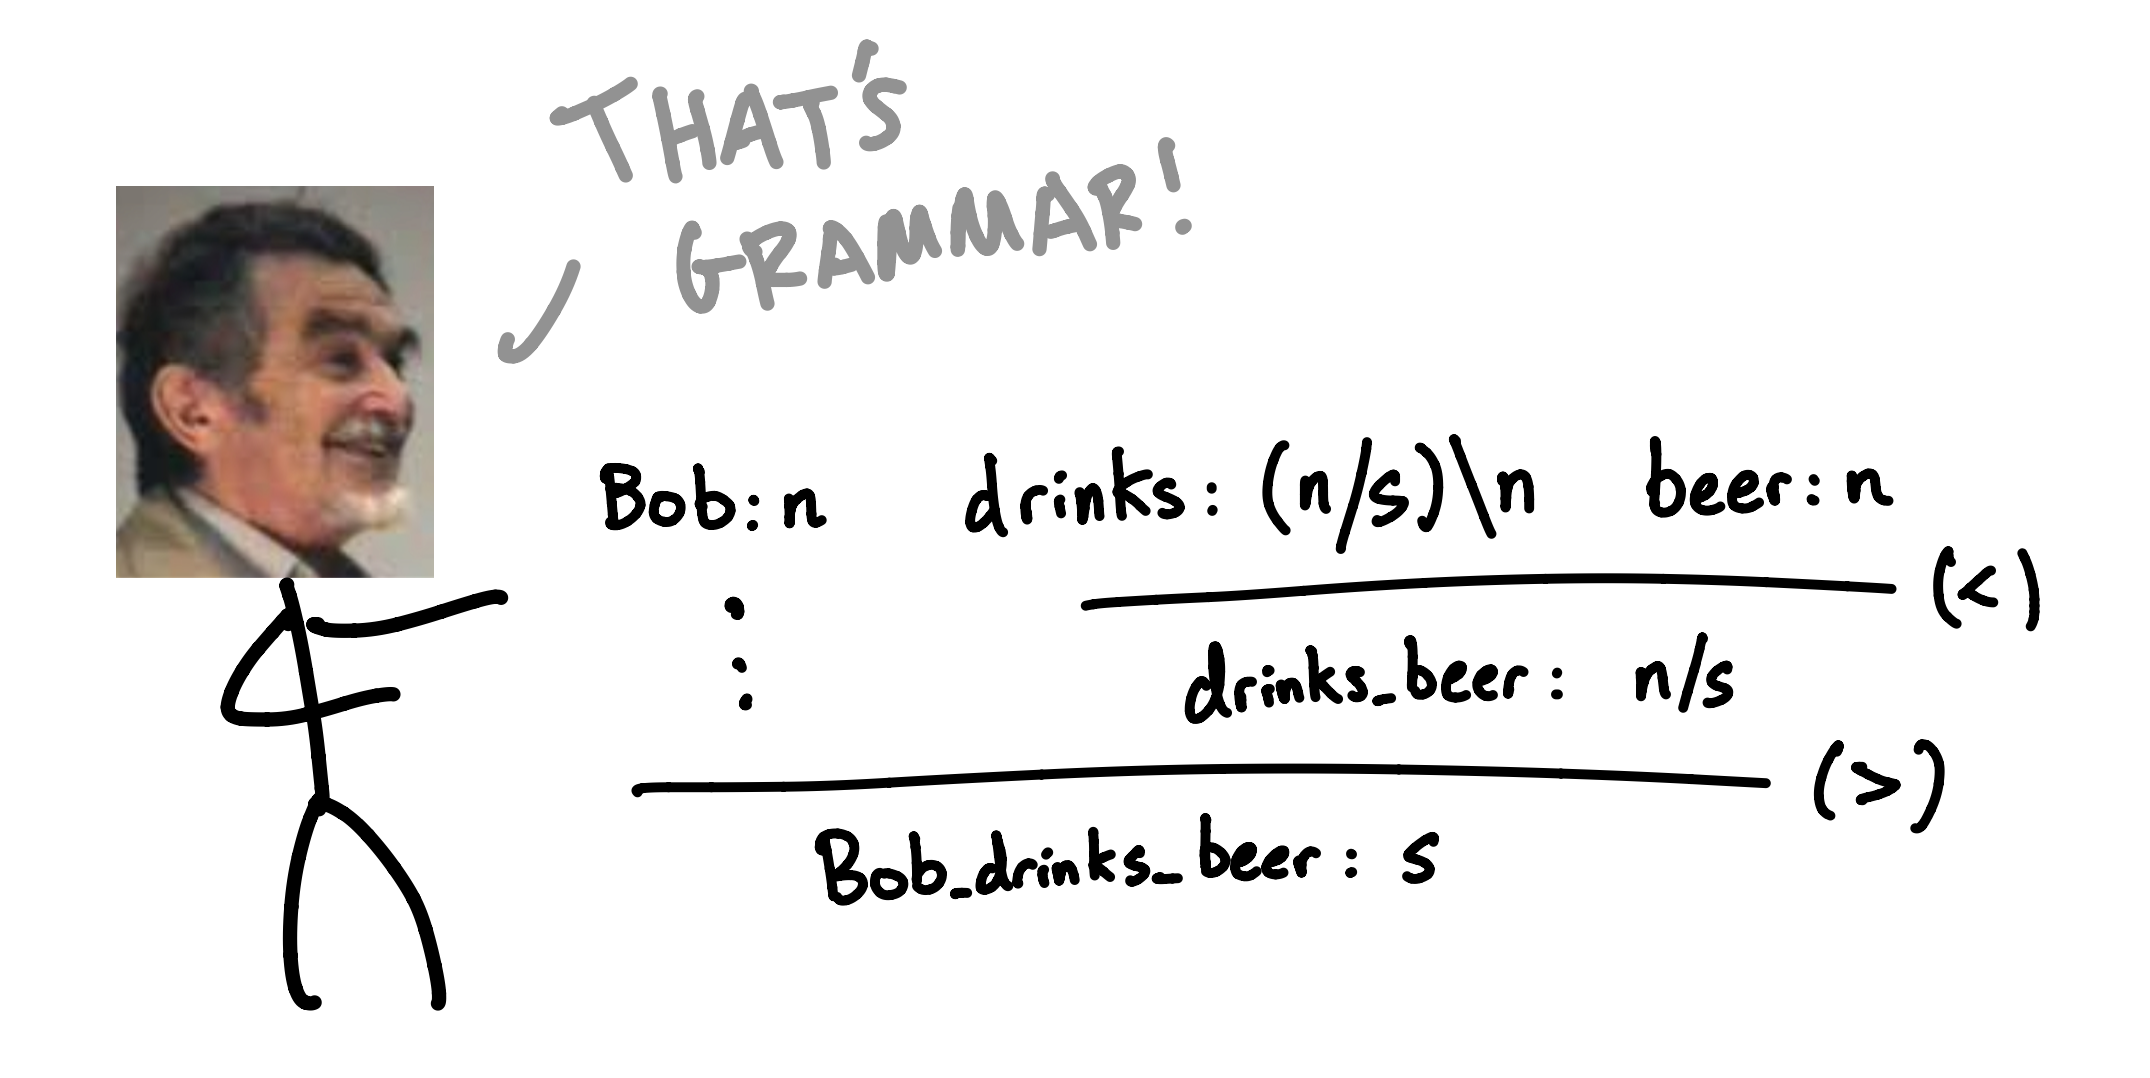
\includegraphics{figures/cartoons/lambek1}}
\caption{In English, we may consider a noun to have type $n$, and a transitive verb $(n/s)\setminus n$, to yield a well-formedness proof of \texttt{Bob drinks beer}. The type formation rules for such a grammar are intuitive. Apart from a stock of basic types $\mathbb{B}$ that contains special final types to indicate sentences, we have two type formation operators $(-/=)$ and $(- \setminus =)$, which along with their elimination rules establish a requirement that grammatical categories require other grammatical categories to their left or right. This is the essence of Lambek's calculi \textbf{NL} and \textbf{L}. CCGs keep the same minimal type-formations, but include extra sequent rules such as type-raising and cross-composition.}
\end{figure}

\begin{figure}[h!]
\centering
\scalebox{1}{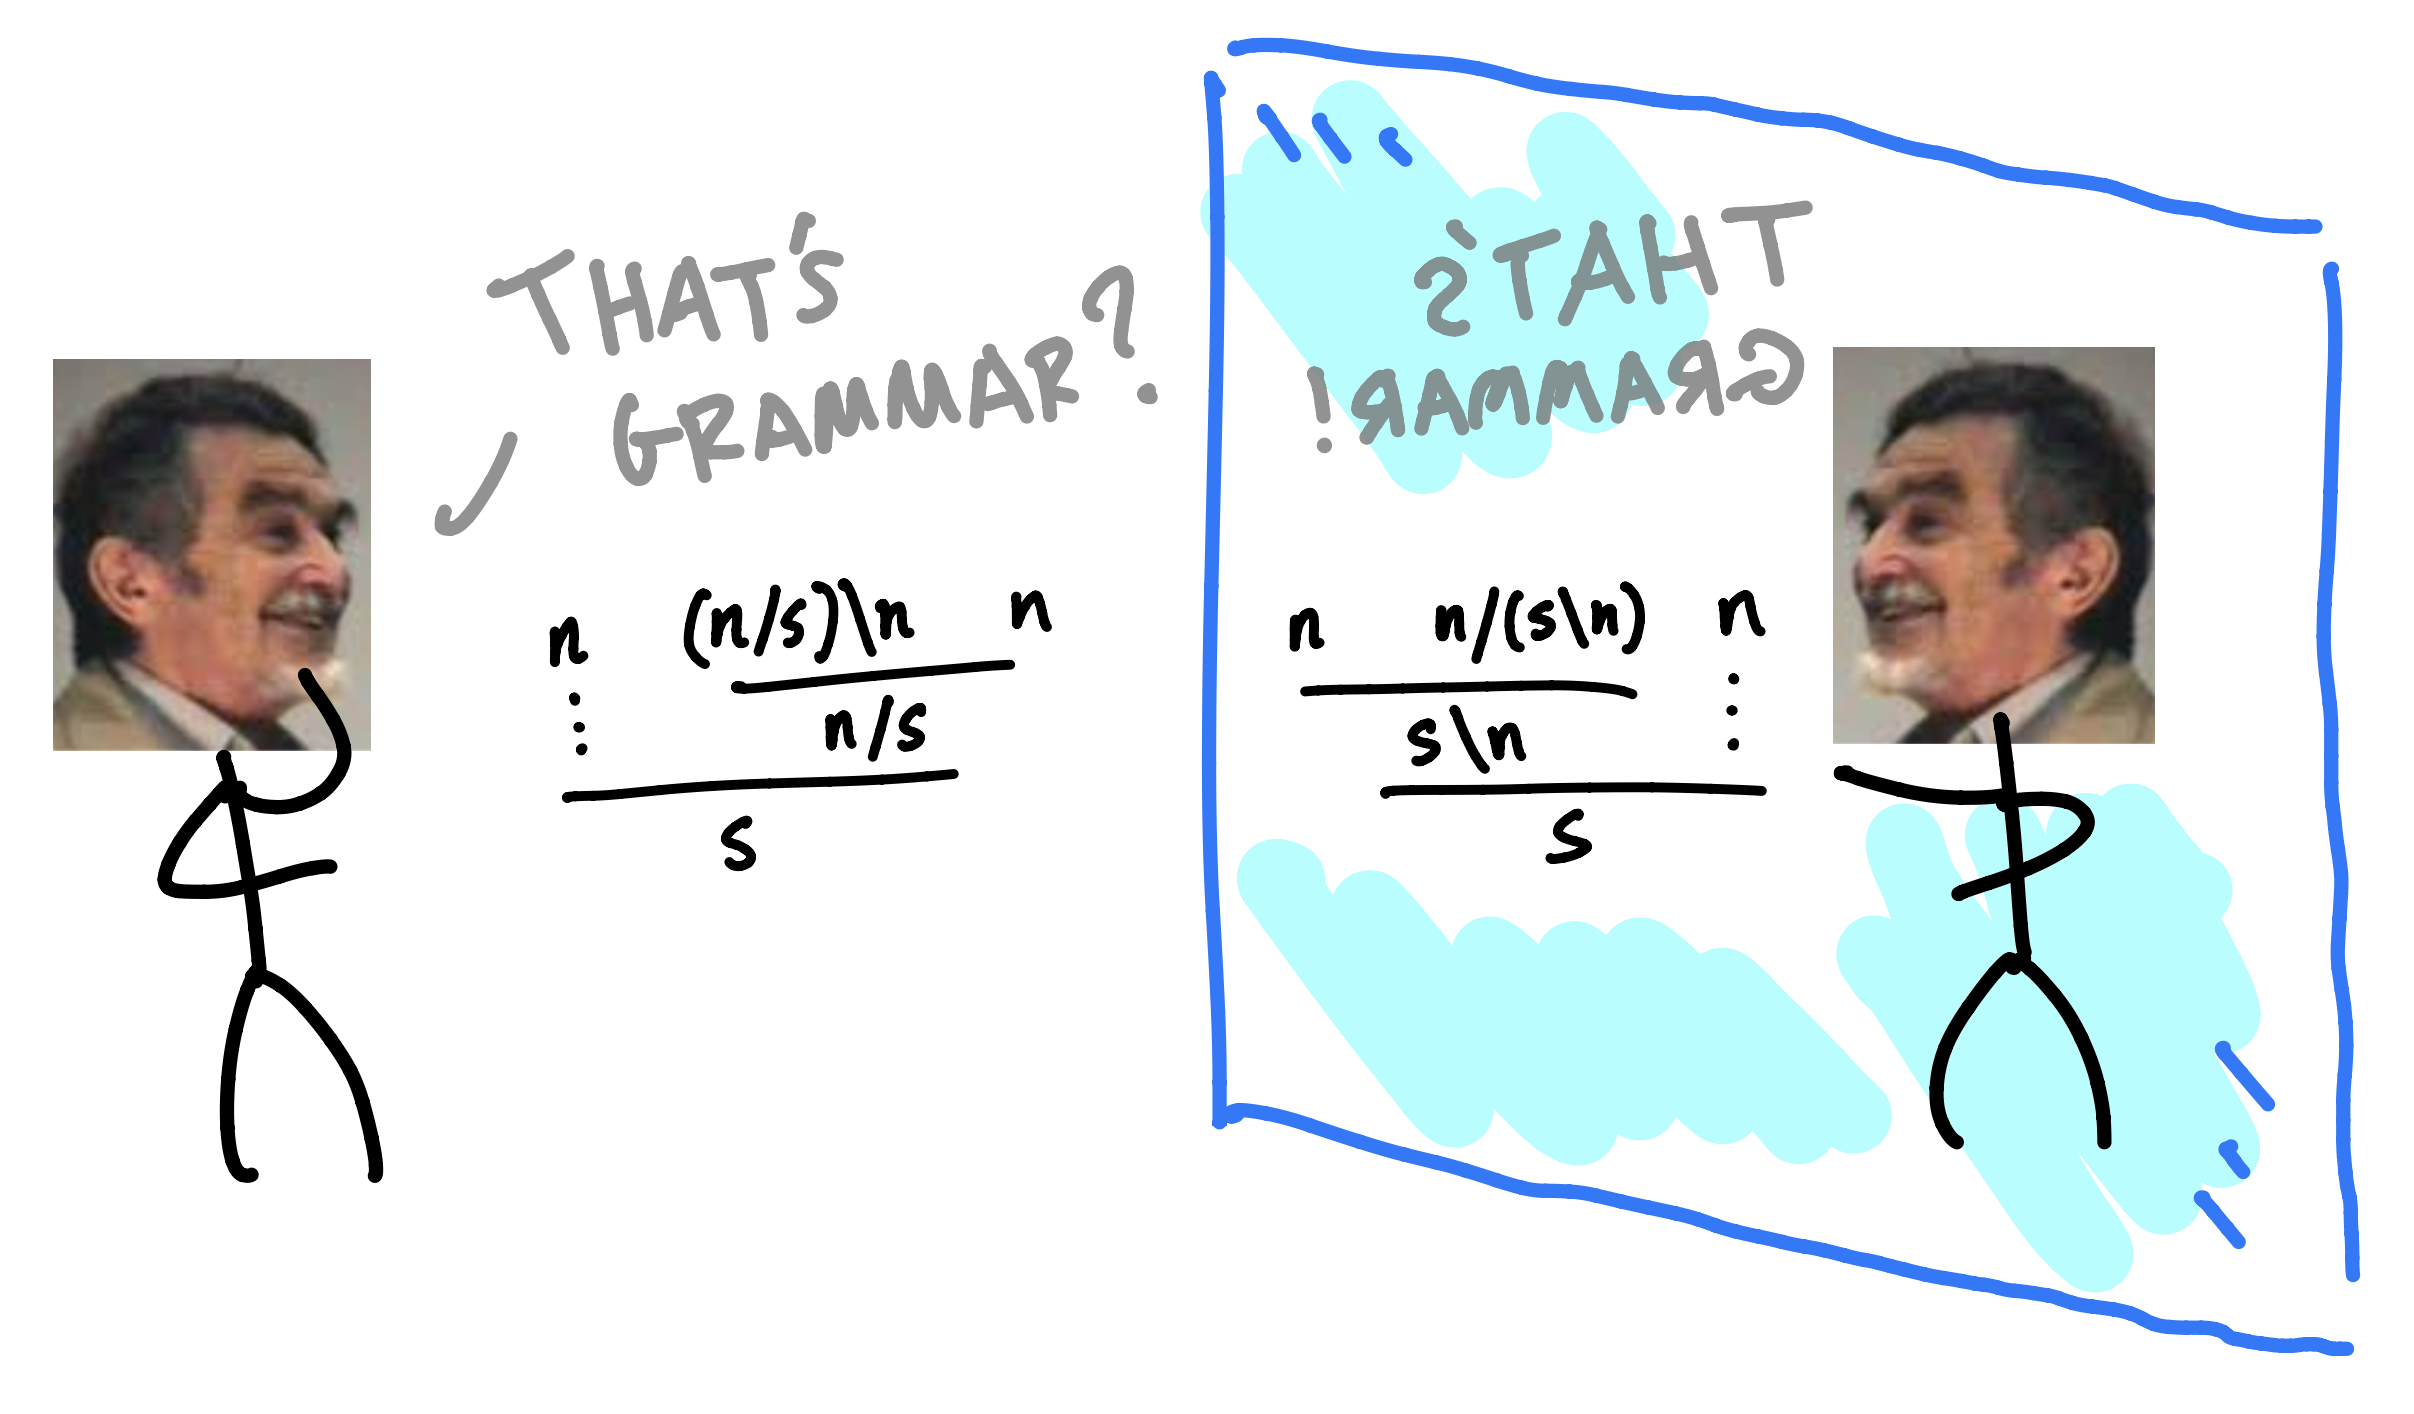
\includegraphics{figures/cartoons/lambek2}}
\caption{We can notice an asymmetry in the above formulation when we examine the transitive verb type $(n/s)\setminus n$ again; it asks first for a noun to the right, and then a noun to the left. We could just as well have asked for the nouns in the other order with the typing $(n/s)\setminus n$ and obtained all of the same proofs.}
\end{figure}

\begin{figure}[h!]
\centering
\scalebox{1}{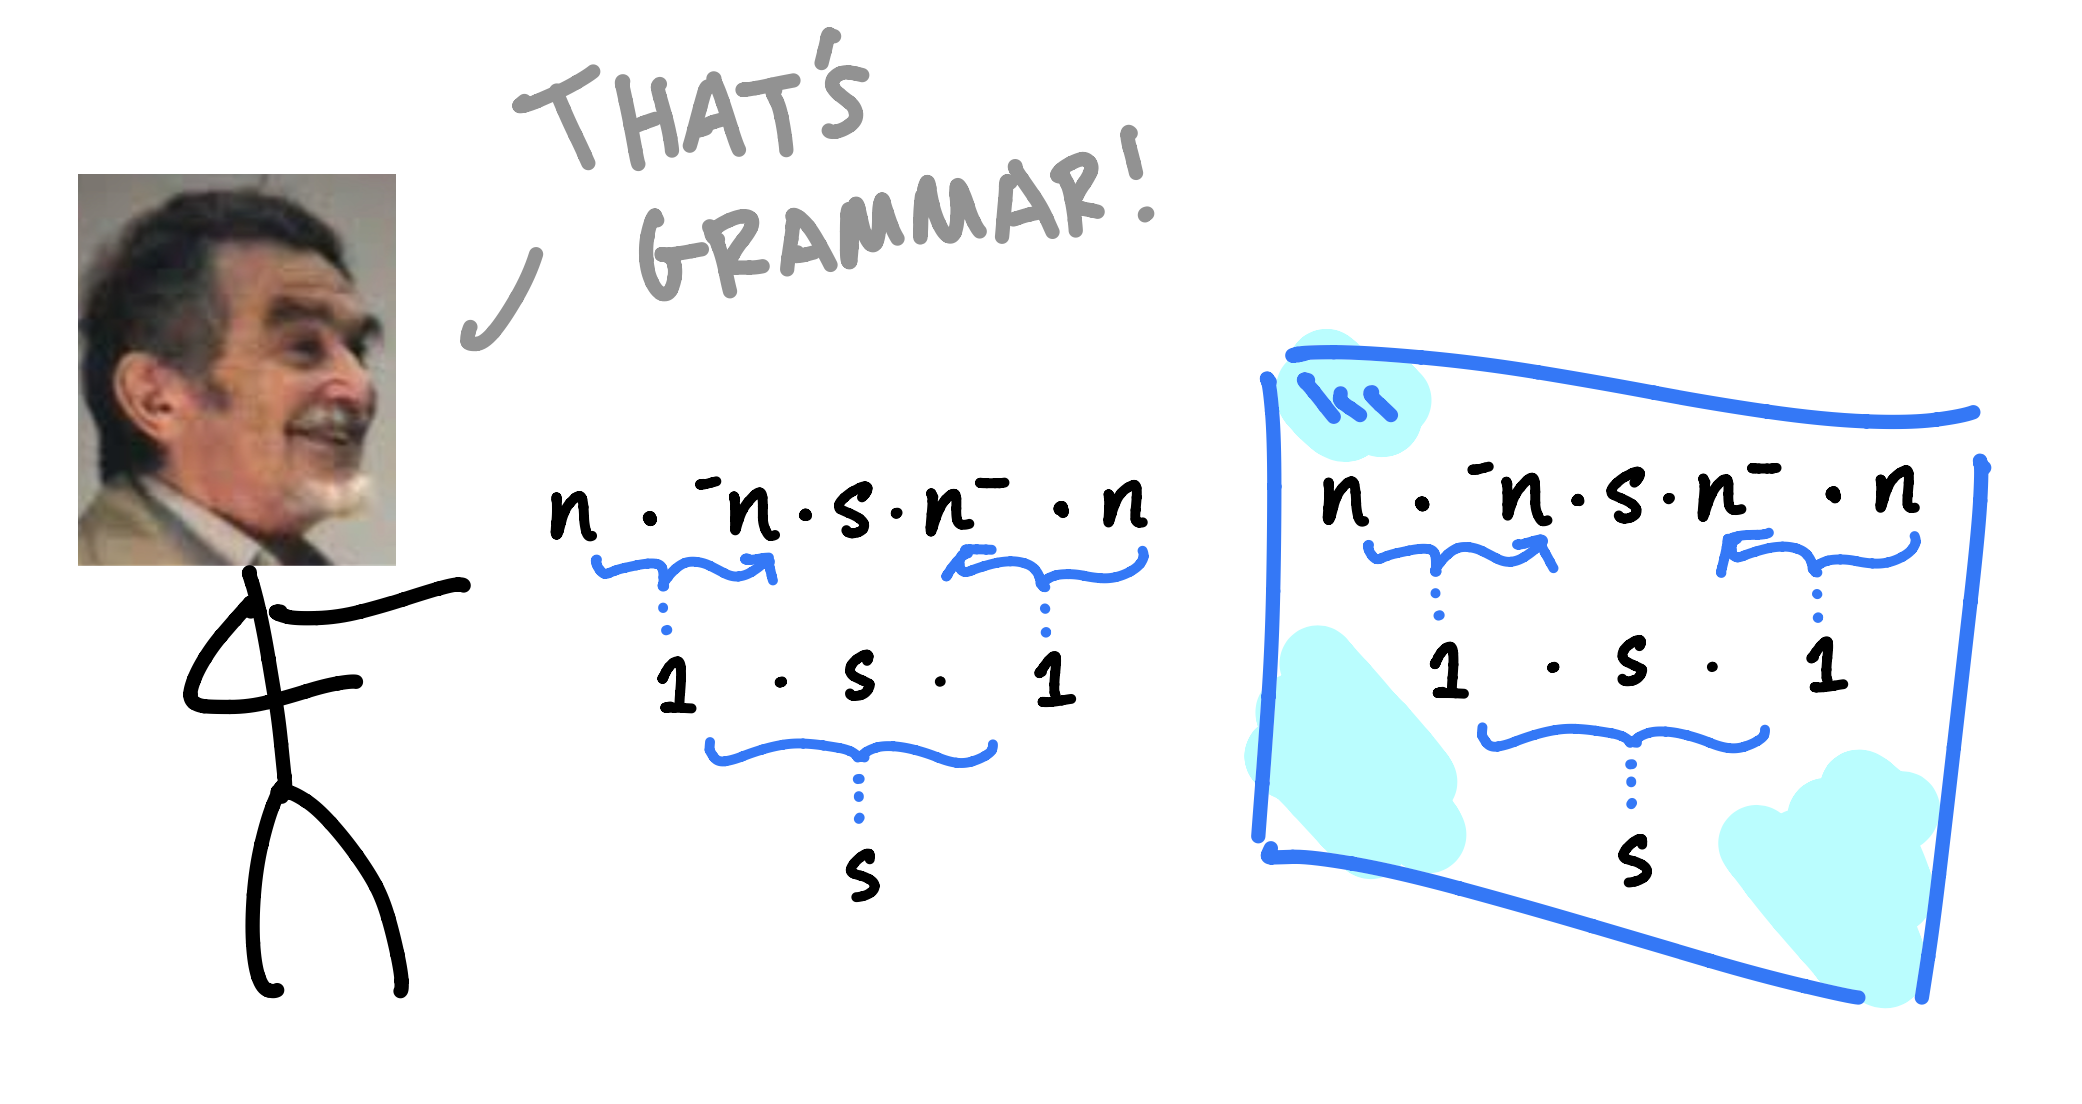
\includegraphics{figures/cartoons/lambek3}}
\caption{To eliminate this asymmetry, Lambek devised pregroup grammars. Whereas a group is a monoid with inverses up to left- and right-multiplication, a pregroup weakens the requirement for inverses so that all elements have distinct left- and right- inverses, denoted $x^{-1}$ and $^{-1}x$ respectively. Eliminating or introducing inverses is a non-identity relation on elements of the pregroup, so we have axioms of the form e.g. $x \cdot ^{-1}x \rightarrow 1 \rightarrow ^{1}x \cdot x$. In this formulation, denoting the multiplication with a dot, both $(n/s)\setminus n$ and $(n/s)\setminus n$ become $^{-1}n \cdot s \cdot n^{-1}$, which just wants a noun to the left and a noun to the right in whatever order to eliminate the flanking inverses to reveal the embedded sentence type. Now we can obtain the same proof of correctness as a series of algebraic reductions.

\begin{align*}
& &n \cdot (^{-1}n \cdot s \cdot n^{-1}) \cdot n\\
&\rightarrow &(n \cdot ^{-1}n) \cdot s \cdot (n^{-1} \cdot n)\\
&\rightarrow & 1 \cdot s \cdot 1\\
&\rightarrow & s
\end{align*}
}
\end{figure}
\clearpage

\subsection{Coecke's Composition}

\begin{figure}[h!]
\centering
\scalebox{0.9}{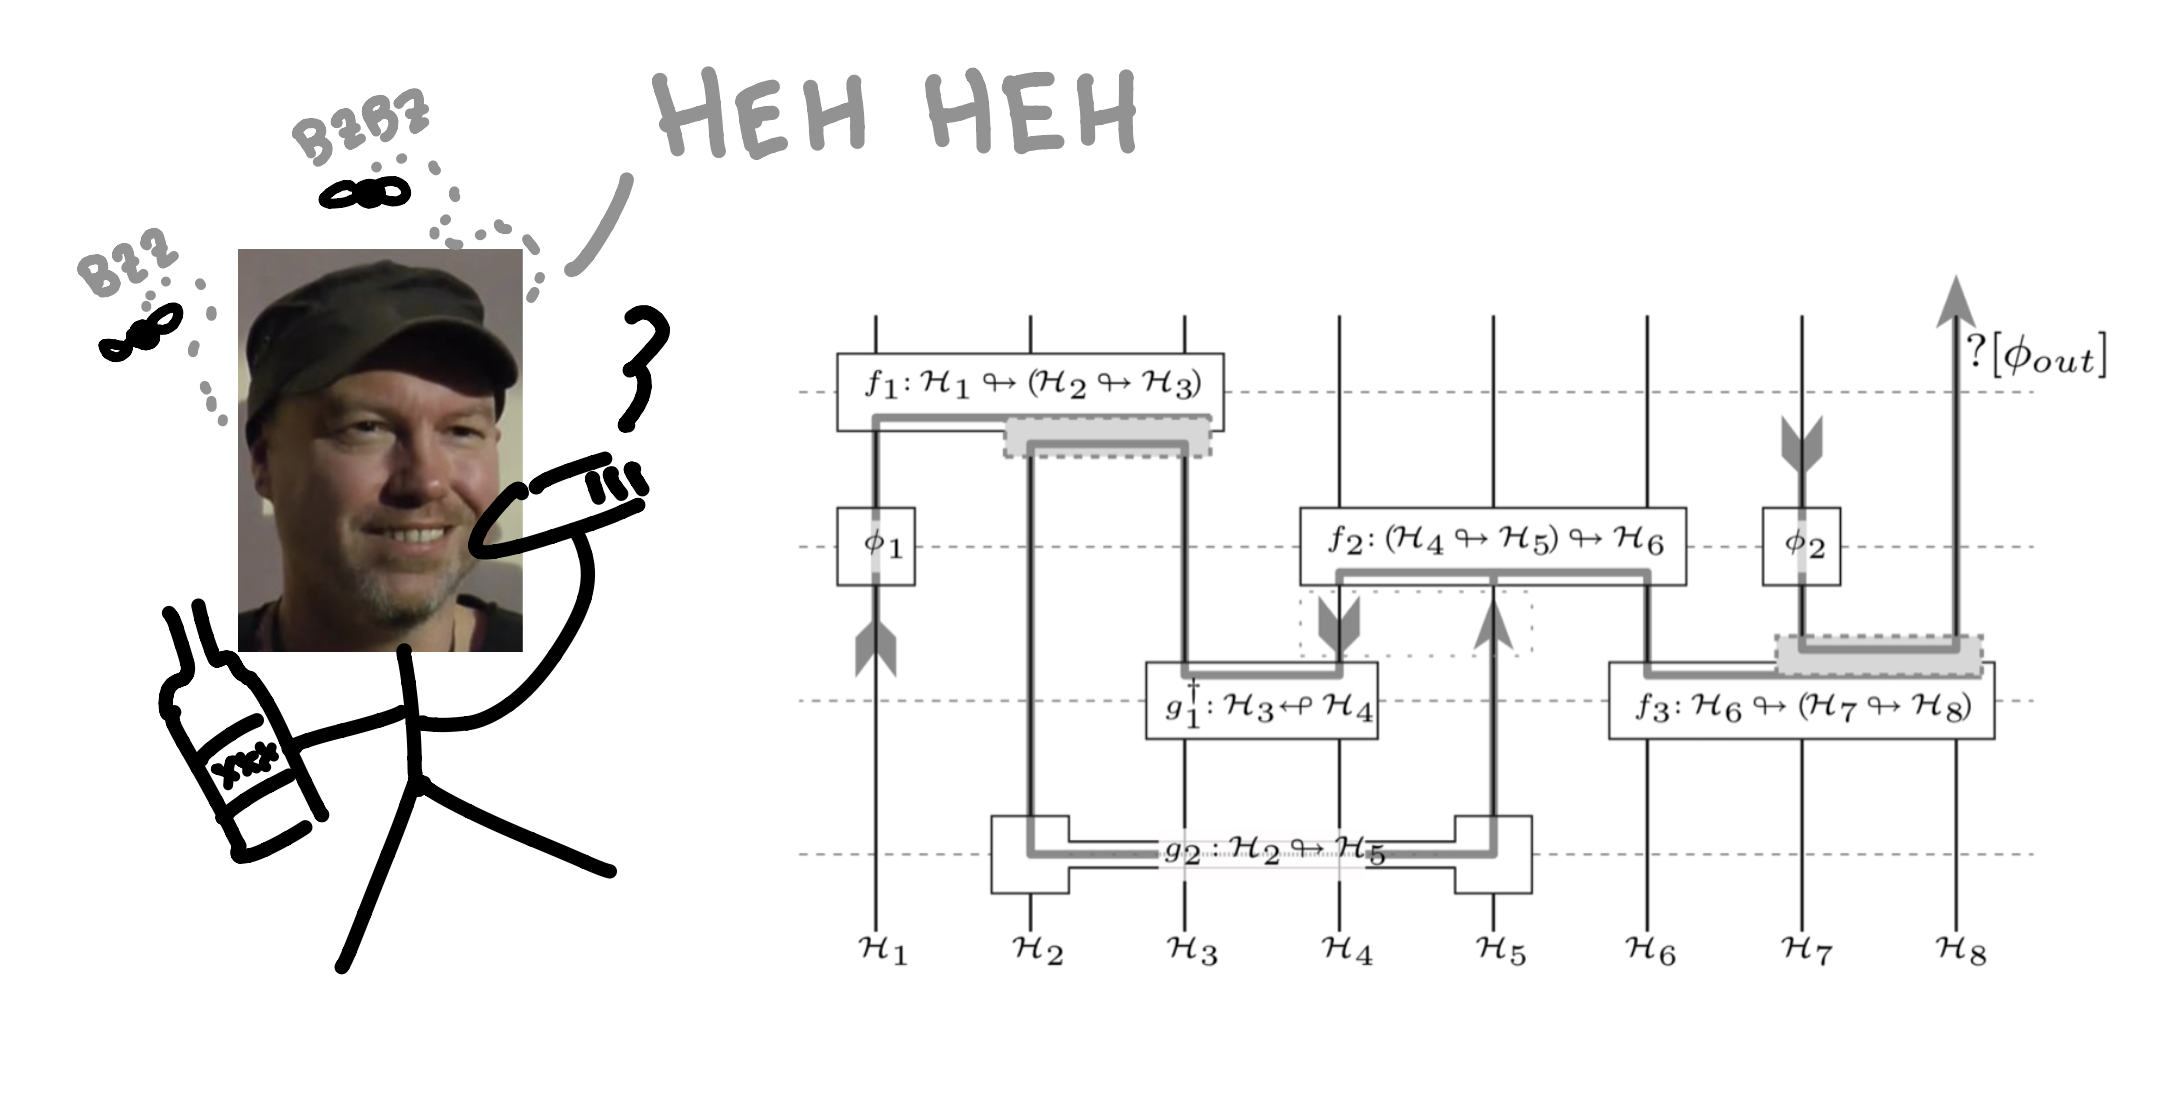
\includegraphics{figures/cartoons/bob1}}
\caption{Meanwhile, an underground grunge vagabond moonlighting as a quantum physicist moonlighting as a computer scientist was causing a shortage of cigars and whiskey in a small English town. He noticed a funny thing about the composition of multiple non-destructive measurements of a quantum system, which was that information could be carried, or flow, between them. So he wrote a paper \bR invitationtoquantum \e, which contained informal diagrams that looked like this.}
\end{figure}

\begin{figure}[h!]
\centering
\scalebox{0.9}{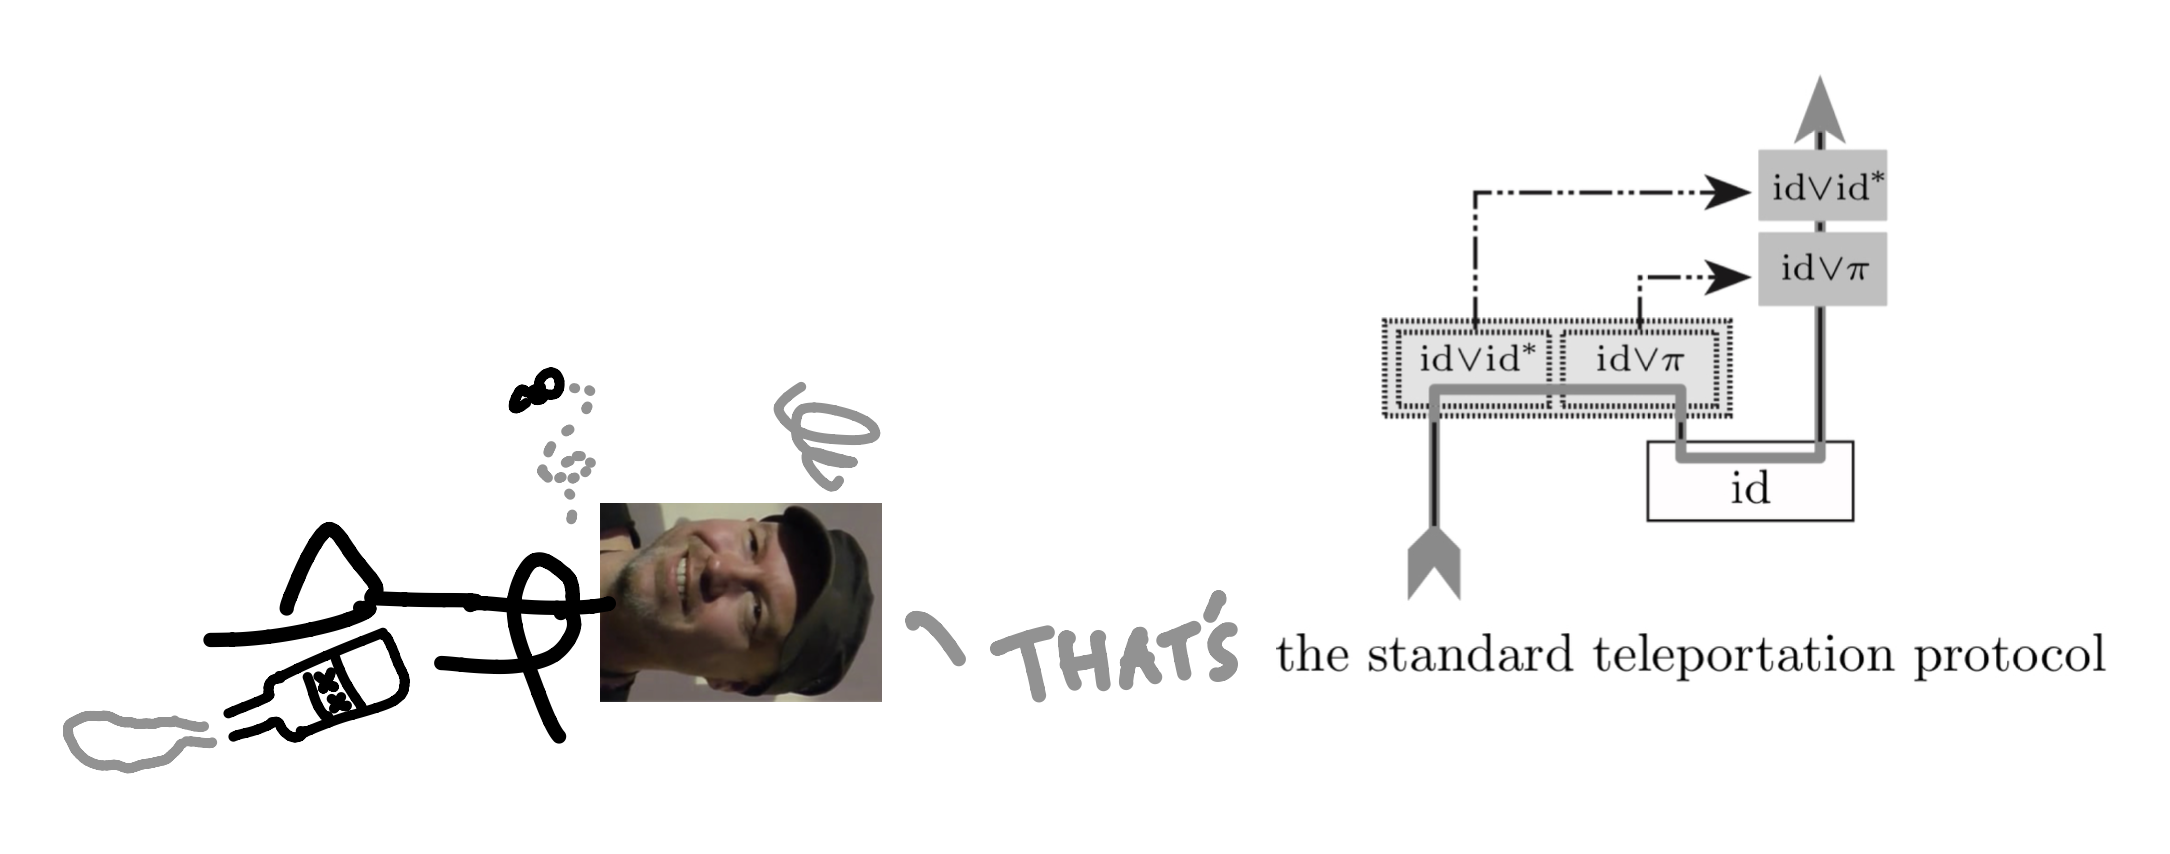
\includegraphics{figures/cartoons/bob2}}
\caption{There were two impressive things about these diagrams. First, the effects such as transparencies for text boxes and curved serifs for angled arrows give a modern feel, but they were done manually in macdraw, the diagrammatic equivalent of sticks and stones. Second, though the diagrams were informal, they provided a way to visualise and reason about entanglement that was impossible by staring at the equivalent matrix formulation of the same composite operator. The most important diagram for our story was this one, which captures the information flow of quantum teleportation.}
\end{figure}
\clearpage

\subsection{Categorical quantum mechanics}

\begin{figure}[h!]
\centering
\scalebox{1}{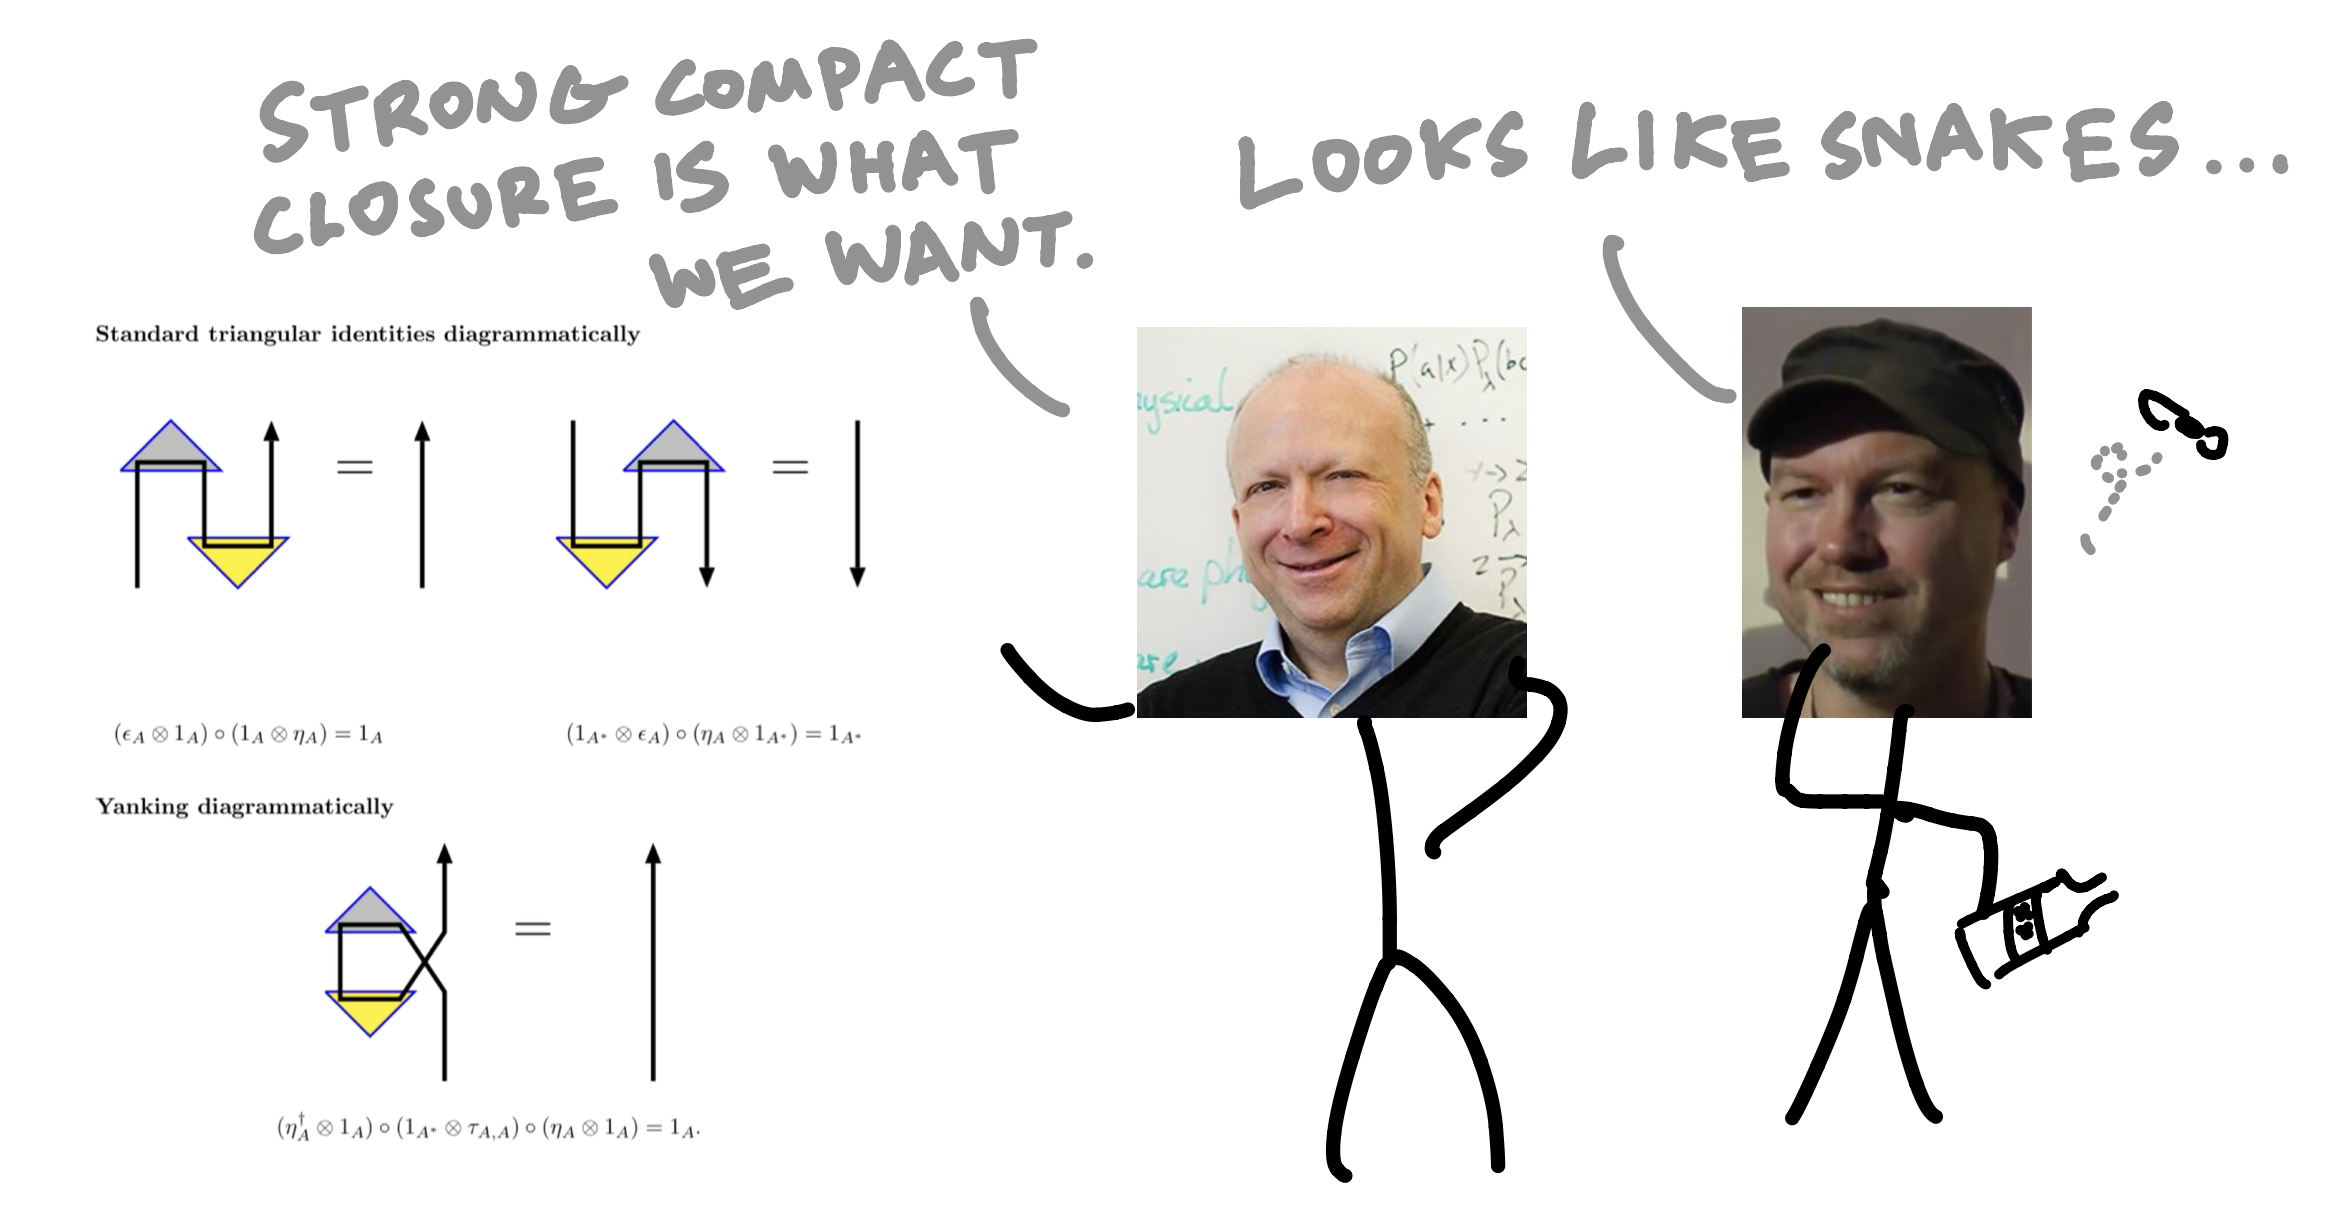
\includegraphics{figures/cartoons/samson}}
\caption{Category theorists and physicists such as Abramsky and Baez were excited about these diagrams, which looked like string diagrams waiting to be made formal. The graphical cups and caps in the important diagram were determined to correspond to a special form of symmetric monoidal closed category called strong compact closed.}
\end{figure}

\begin{figure}[h!]
\centering
\scalebox{1}{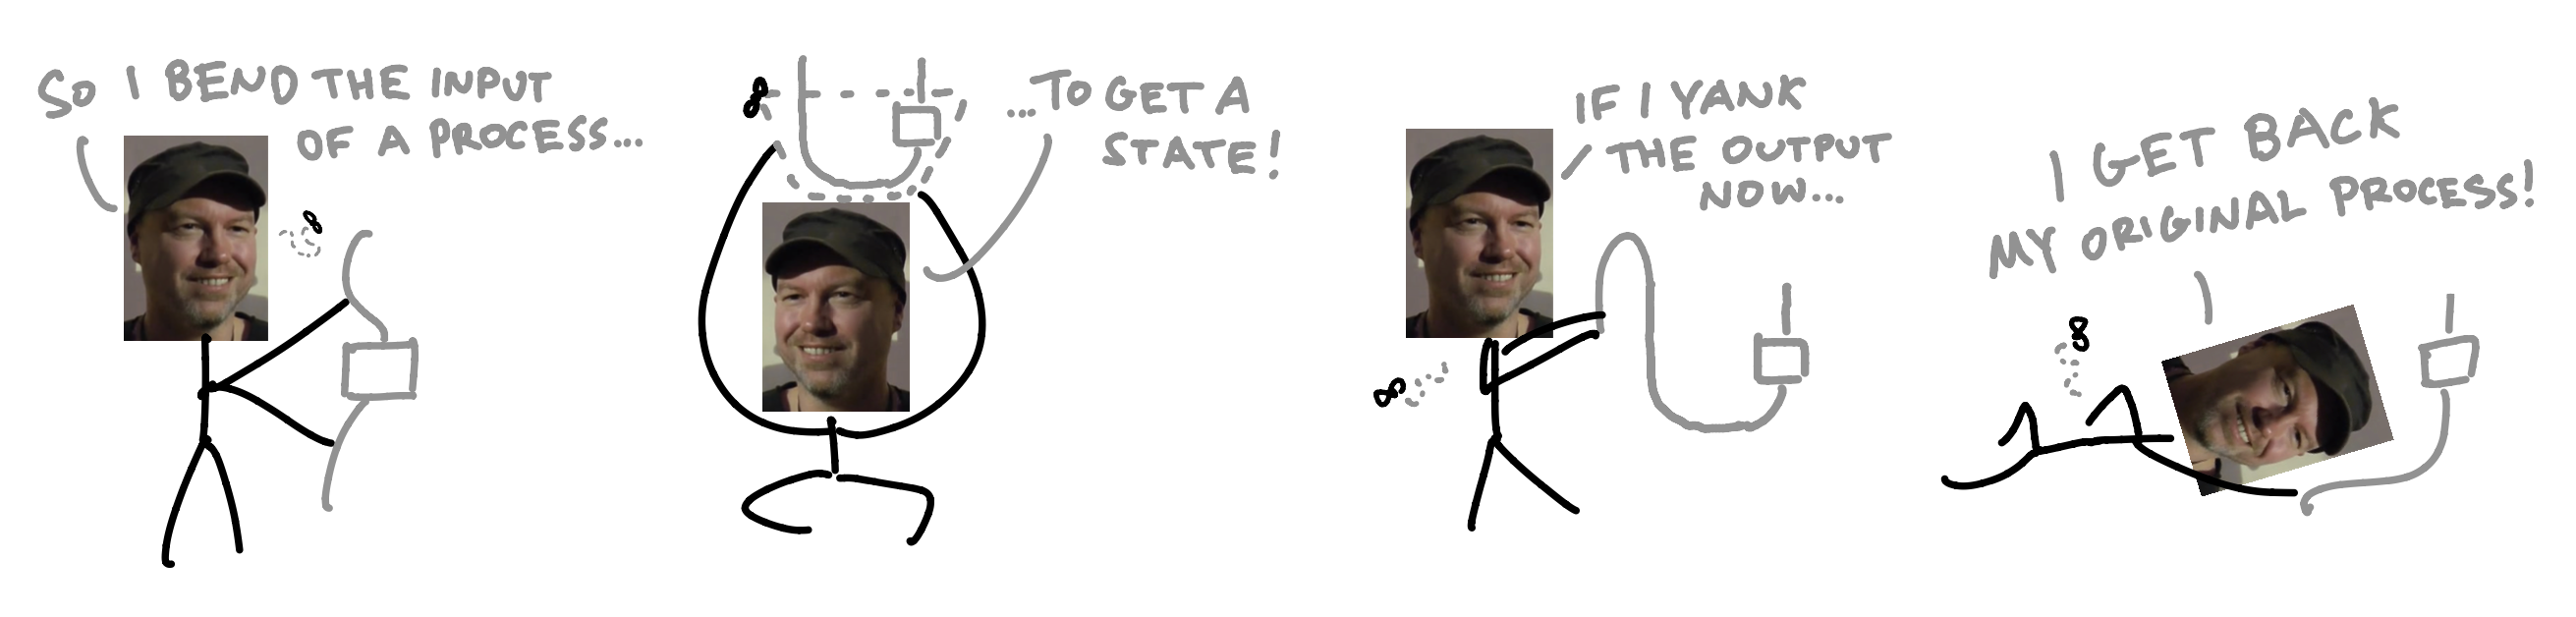
\includegraphics{figures/cartoons/cjiso}}
\caption{Diagrammatically, reasoning in a strongly compact closed category amounts to ignoring the usual requirement of processiveness and forgetting the distinction between inputs and outputs, so that "future" outputs could curl back and be "past" inputs. This formulation also gave insight into the structure of quantum mechanics. For example, the process-state duality of strong compact closure manifested as the Choi–Jamiołkowski isomorphism.}
\end{figure}

\begin{figure}[h!]
\centering
\scalebox{1}{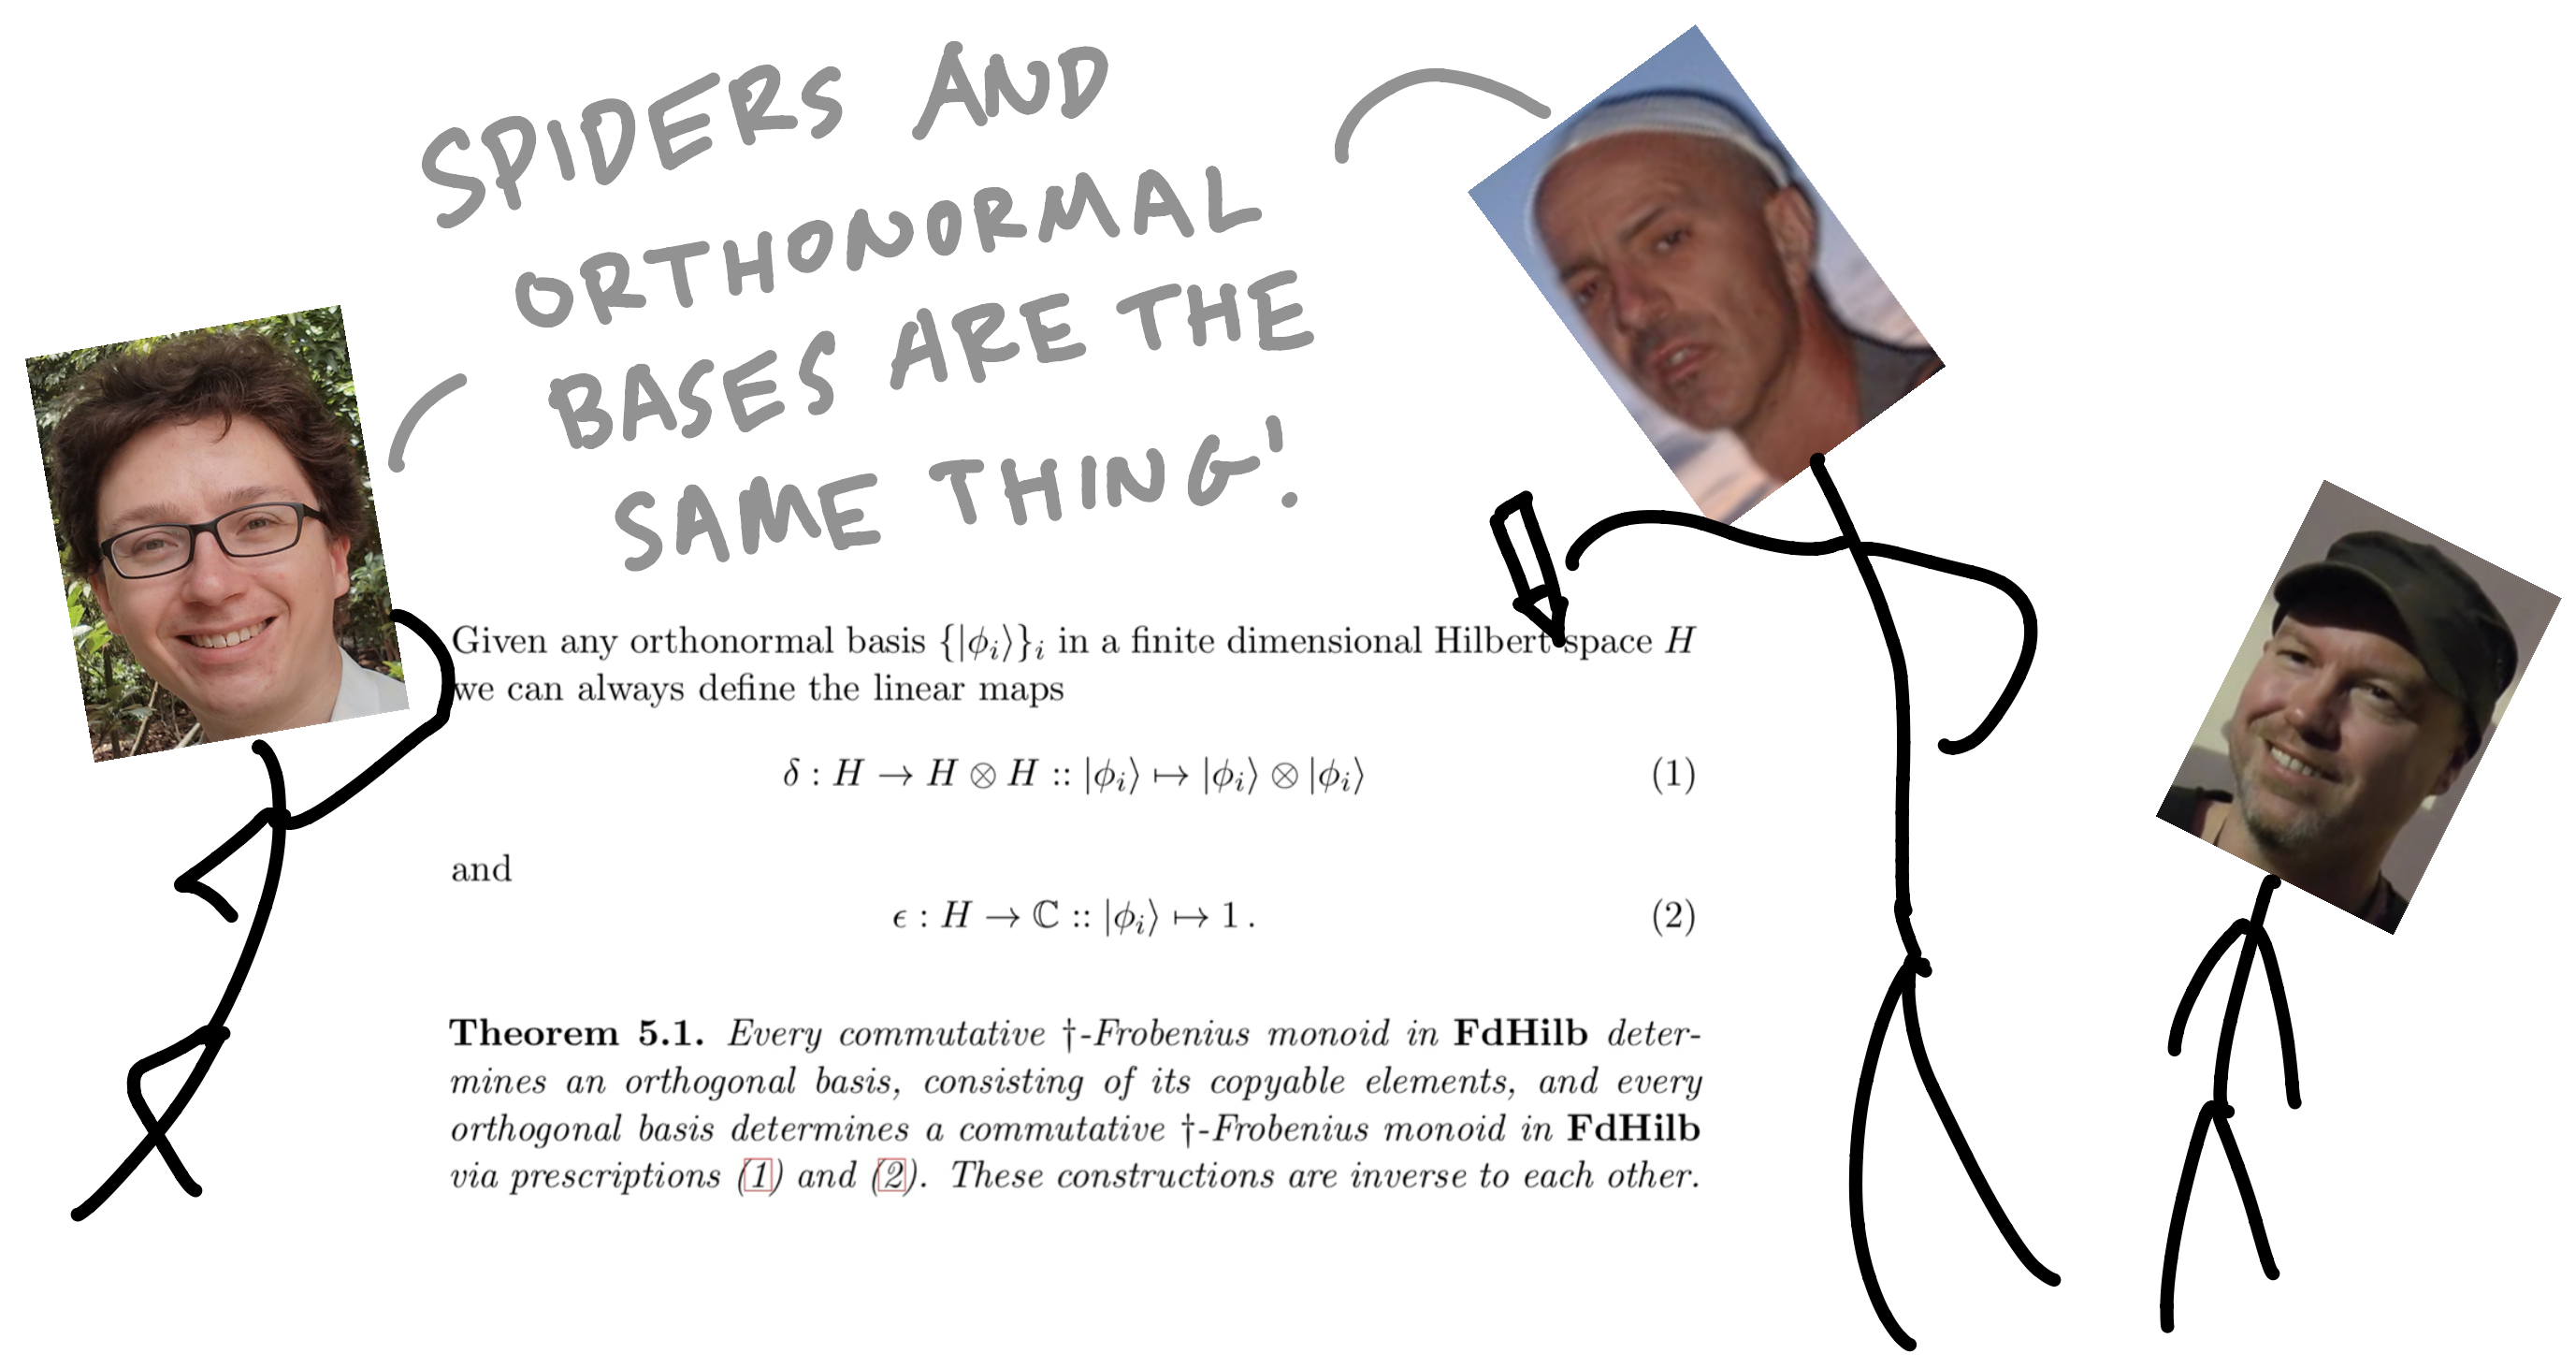
\includegraphics{figures/cartoons/spiders}}
\caption{However, dealing with superpositions necessitated using summation operators within diagrams, which is cumbersome to write especially when dealing with even theoretically simple Bell states. An elegant diagrammatic simplification arose with the observation that special-$\dagger$-frobenius algebras \bR classicquantumstruct \e, or spiders, correspond to choices of orthonormal bases \bR novelchar \e in \textbf{FdHilb}, the ambient setting of finite-dimensional hilbert spaces. Not only did this remove the need for summation operators, it also revealed that strong compact closure was a derived, rather than fundamental structure, since spiders induce compact closed structure.}
\end{figure}

\begin{figure}[h!]
\centering
\scalebox{1}{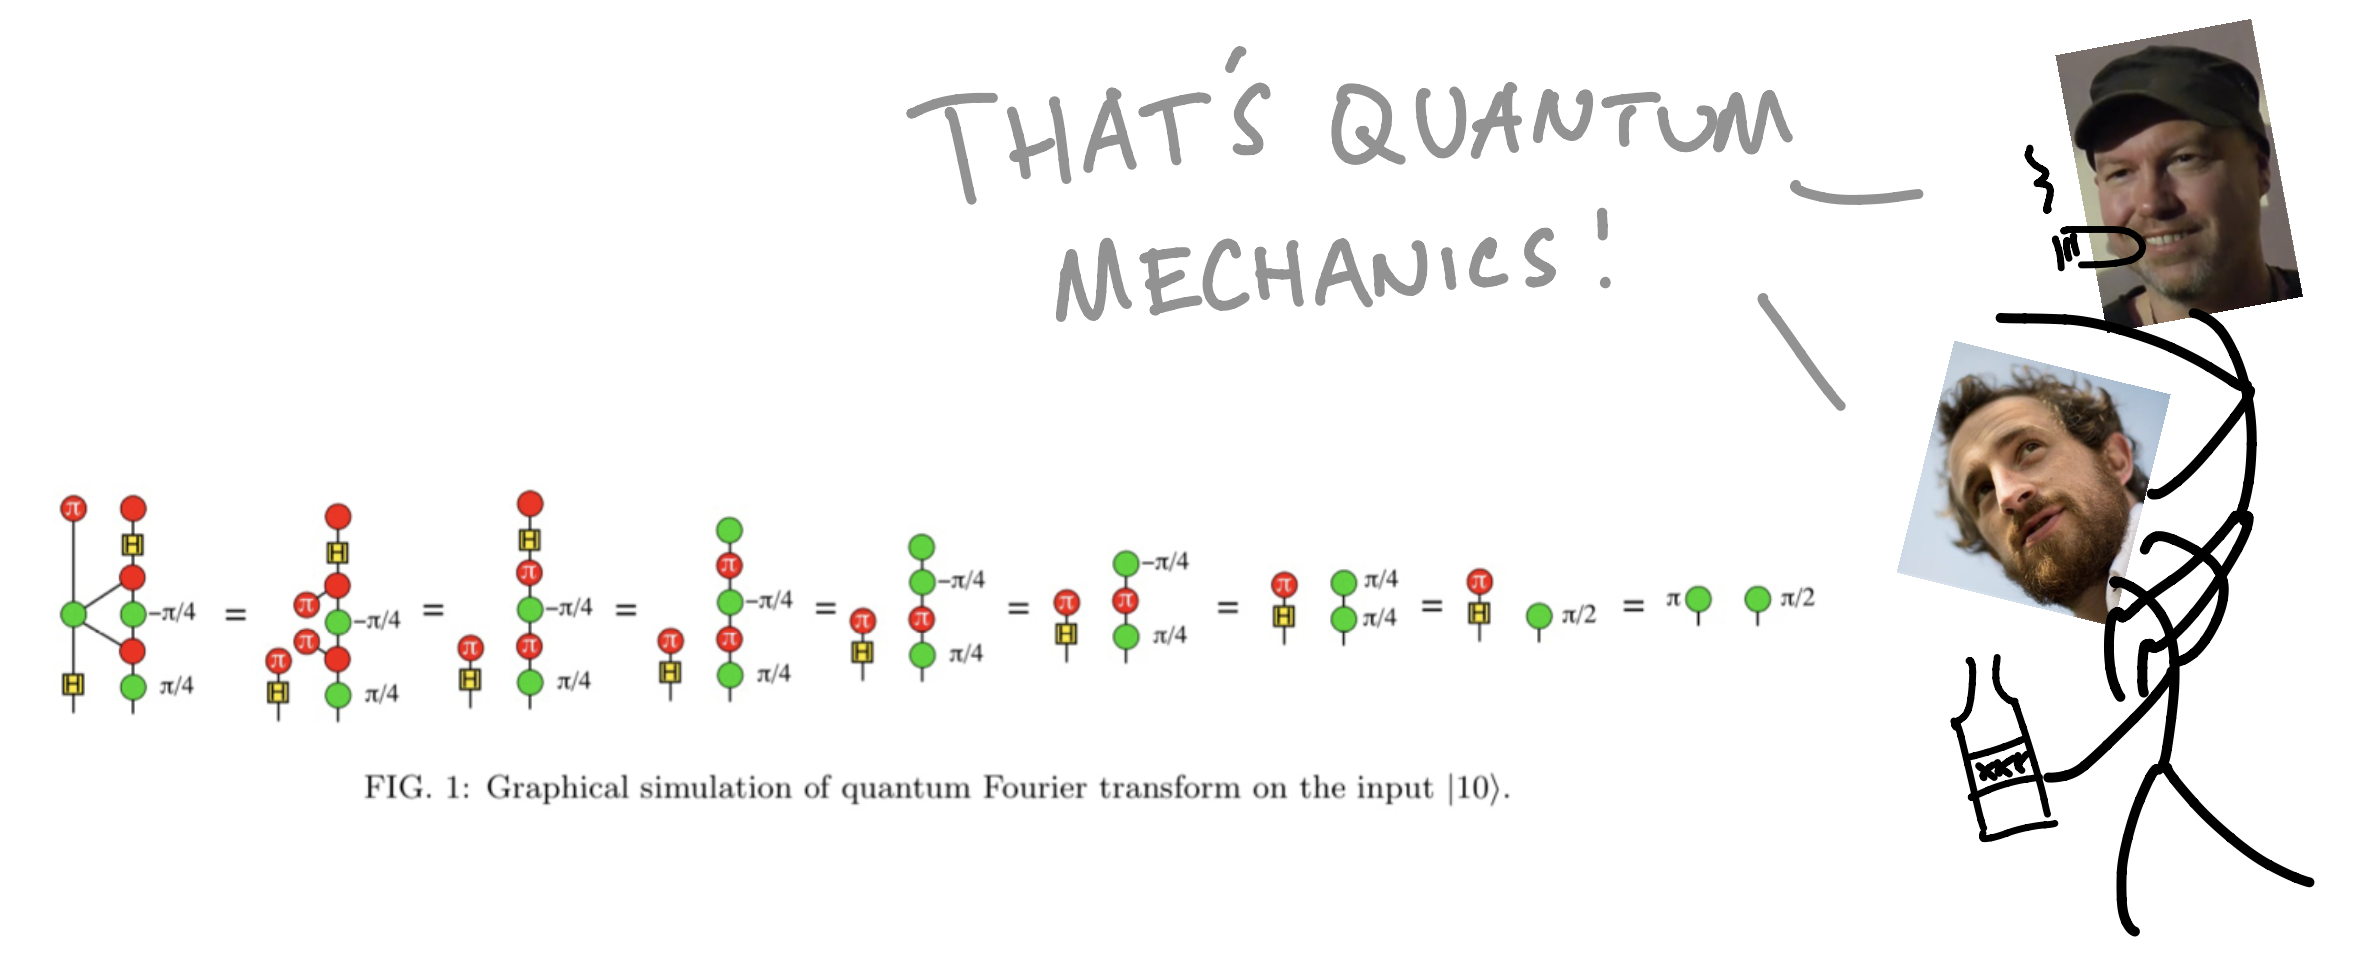
\includegraphics{figures/cartoons/ross}}
\caption{And so the stage was set for a purely diagrammatic treatment of ZX quantum mechanics. The story of ZX diverges away from our interest, so I will summarise what happened afterwards. In no particular order, the development of ZX went on to accommodate a third axis of measurement to yield a ZXW calculus \bR CITE \e, the systems were proven to be complete \bR CITES \e, there are at the time of writing two expository books \bR CITES \e, and ZX-variants are becoming an industry standard for quantum circuit specification and rewriting \bR CITE \e.}
\end{figure}
\clearpage

\subsection{Enter computational linguistics}

\begin{figure}[h!]
\centering
\scalebox{1}{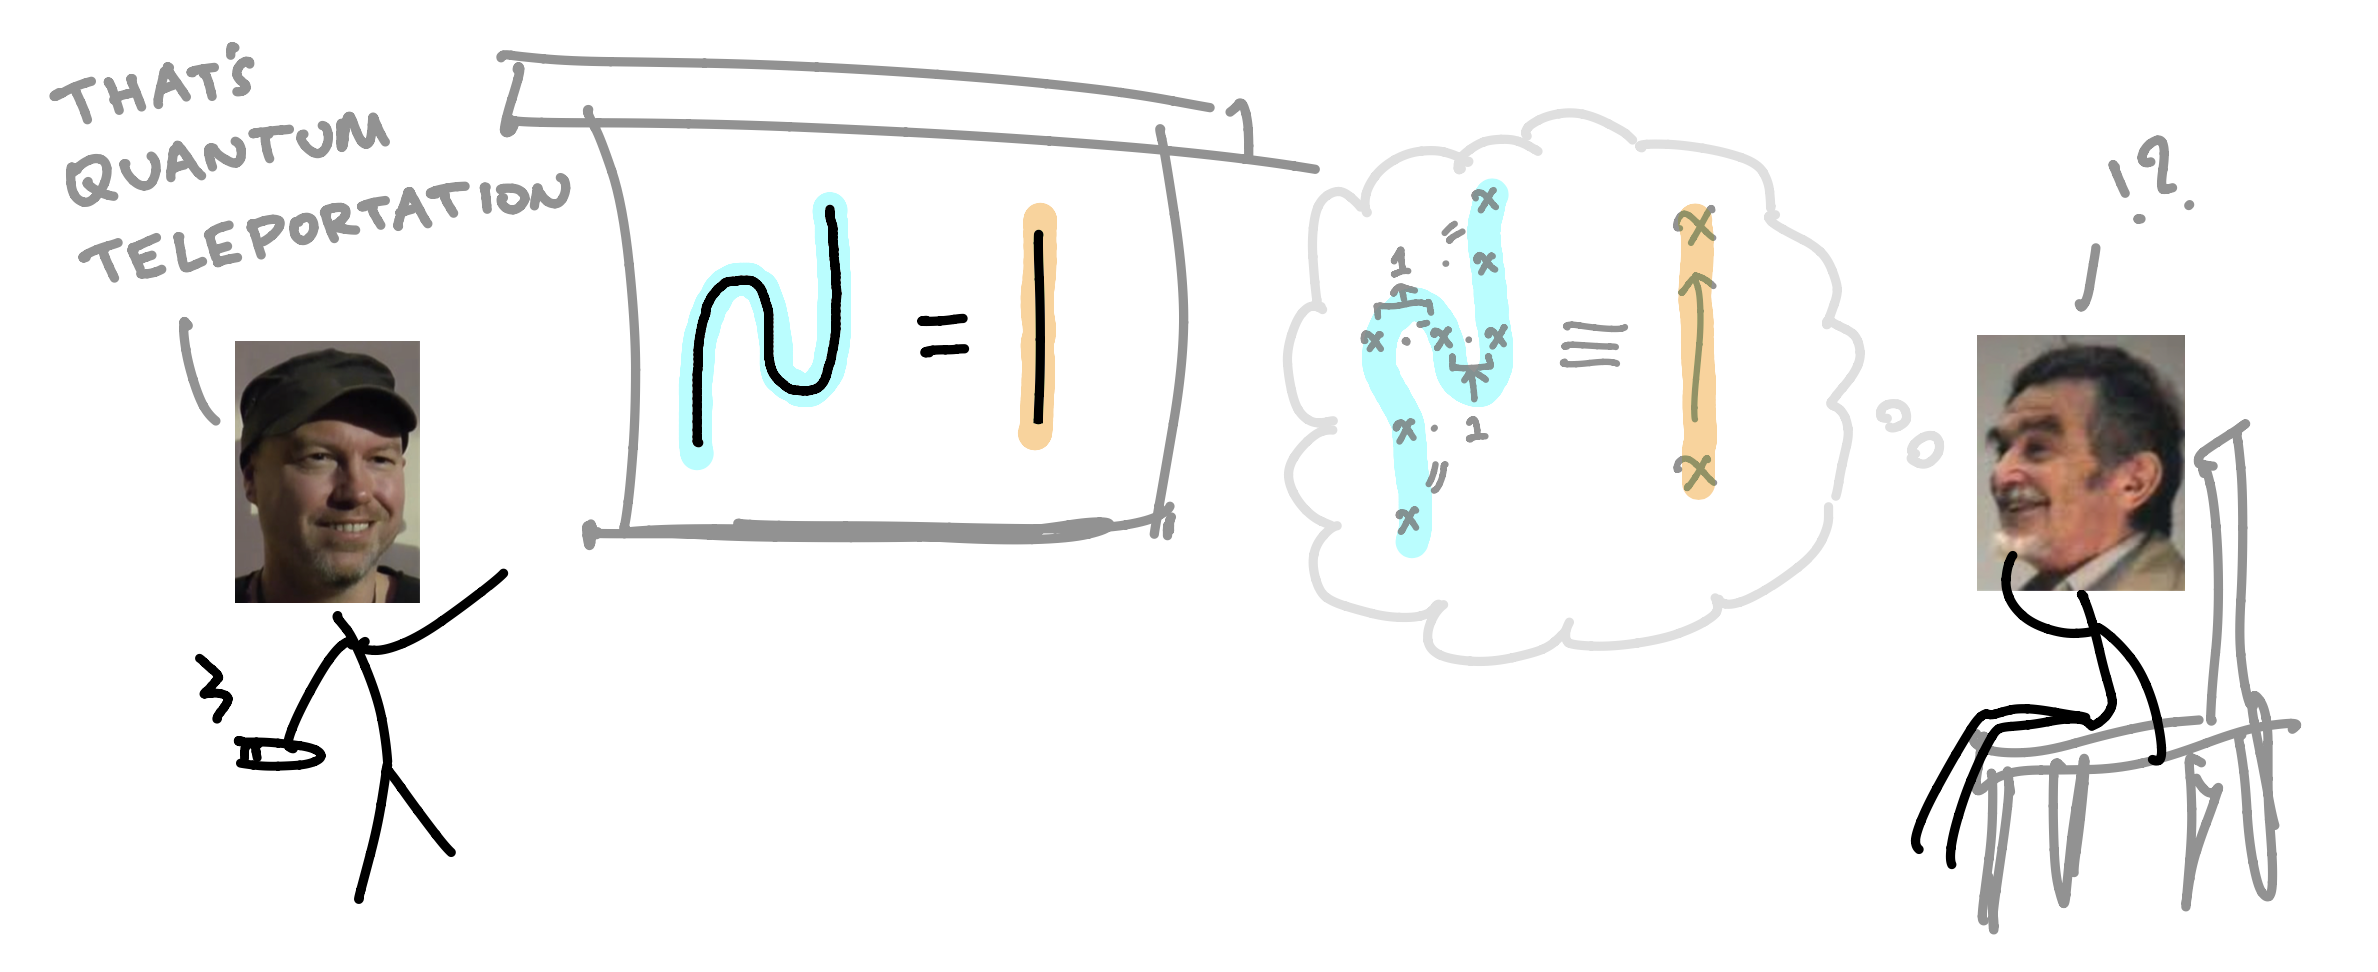
\includegraphics{figures/cartoons/boblambek1}}
\caption{Somewhere in Canada at the turn of the millenium, Bob met Jim, who saw something familiar about the diagram for quantum teleportation. The snake equation for compact closure looked a lot like the categorified version of introducing and eliminating pregroup types.
}
\end{figure}

\begin{figure}[h!]
\centering
\scalebox{1}{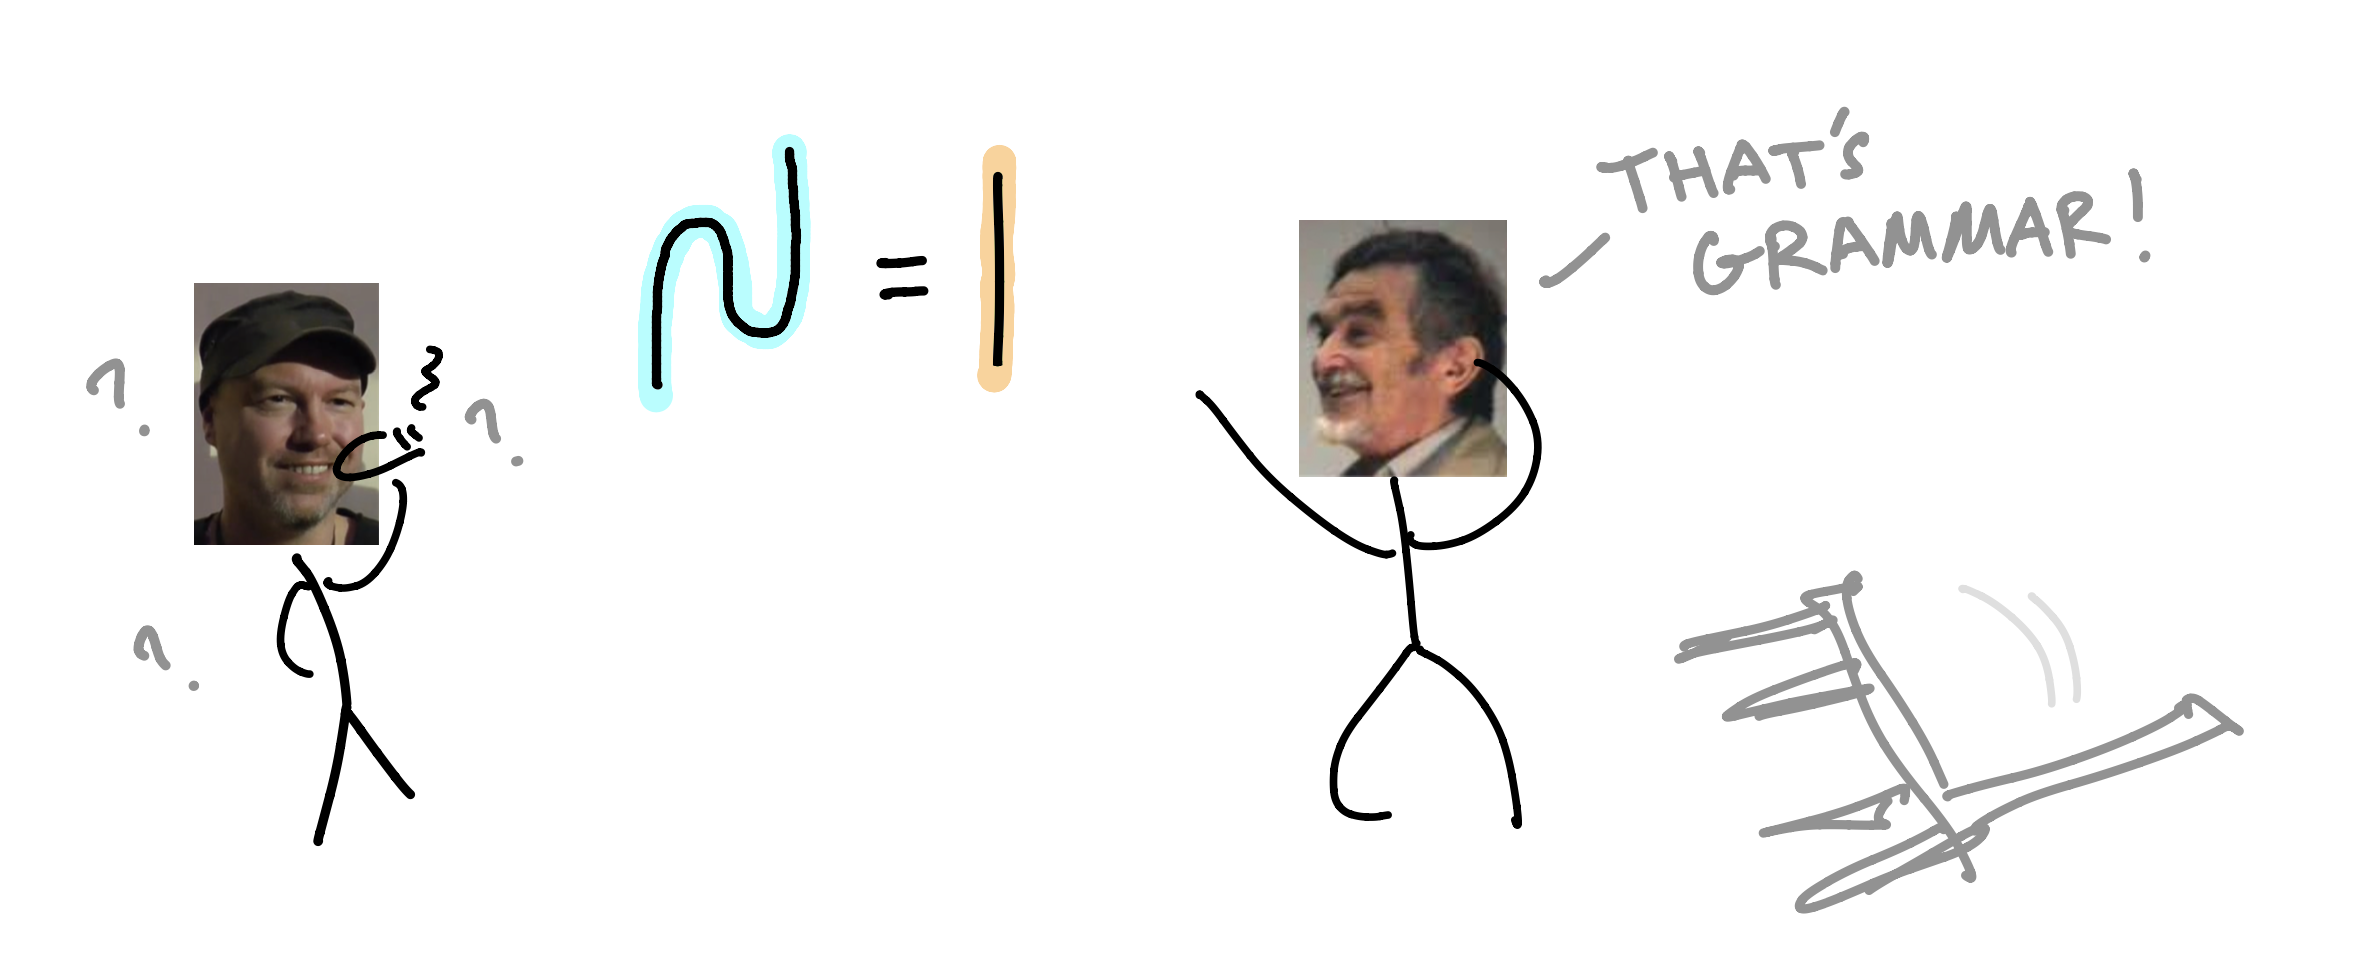
\includegraphics{figures/cartoons/boblambek2}}
\caption{Bob and Jim's meeting put the adjectives \emph{compositional} and \emph{categorical} on the same table, but the cake wasn't ready. Two more actors Steve and Mehrnoosh were required to introduce \emph{distributional}, which refers to Firth's maxim \bR CITE \e "you shall know a word by the company it keeps". In its modern incarnation, this refers generally to vector-based semantics for words, where it is desirable but not necessarily so (as in the case of generic latent space embeddings by an autoencoder) that proximity of vectors models semantic closeness.}
\end{figure}

\begin{figure}[h!]
\centering
\scalebox{1}{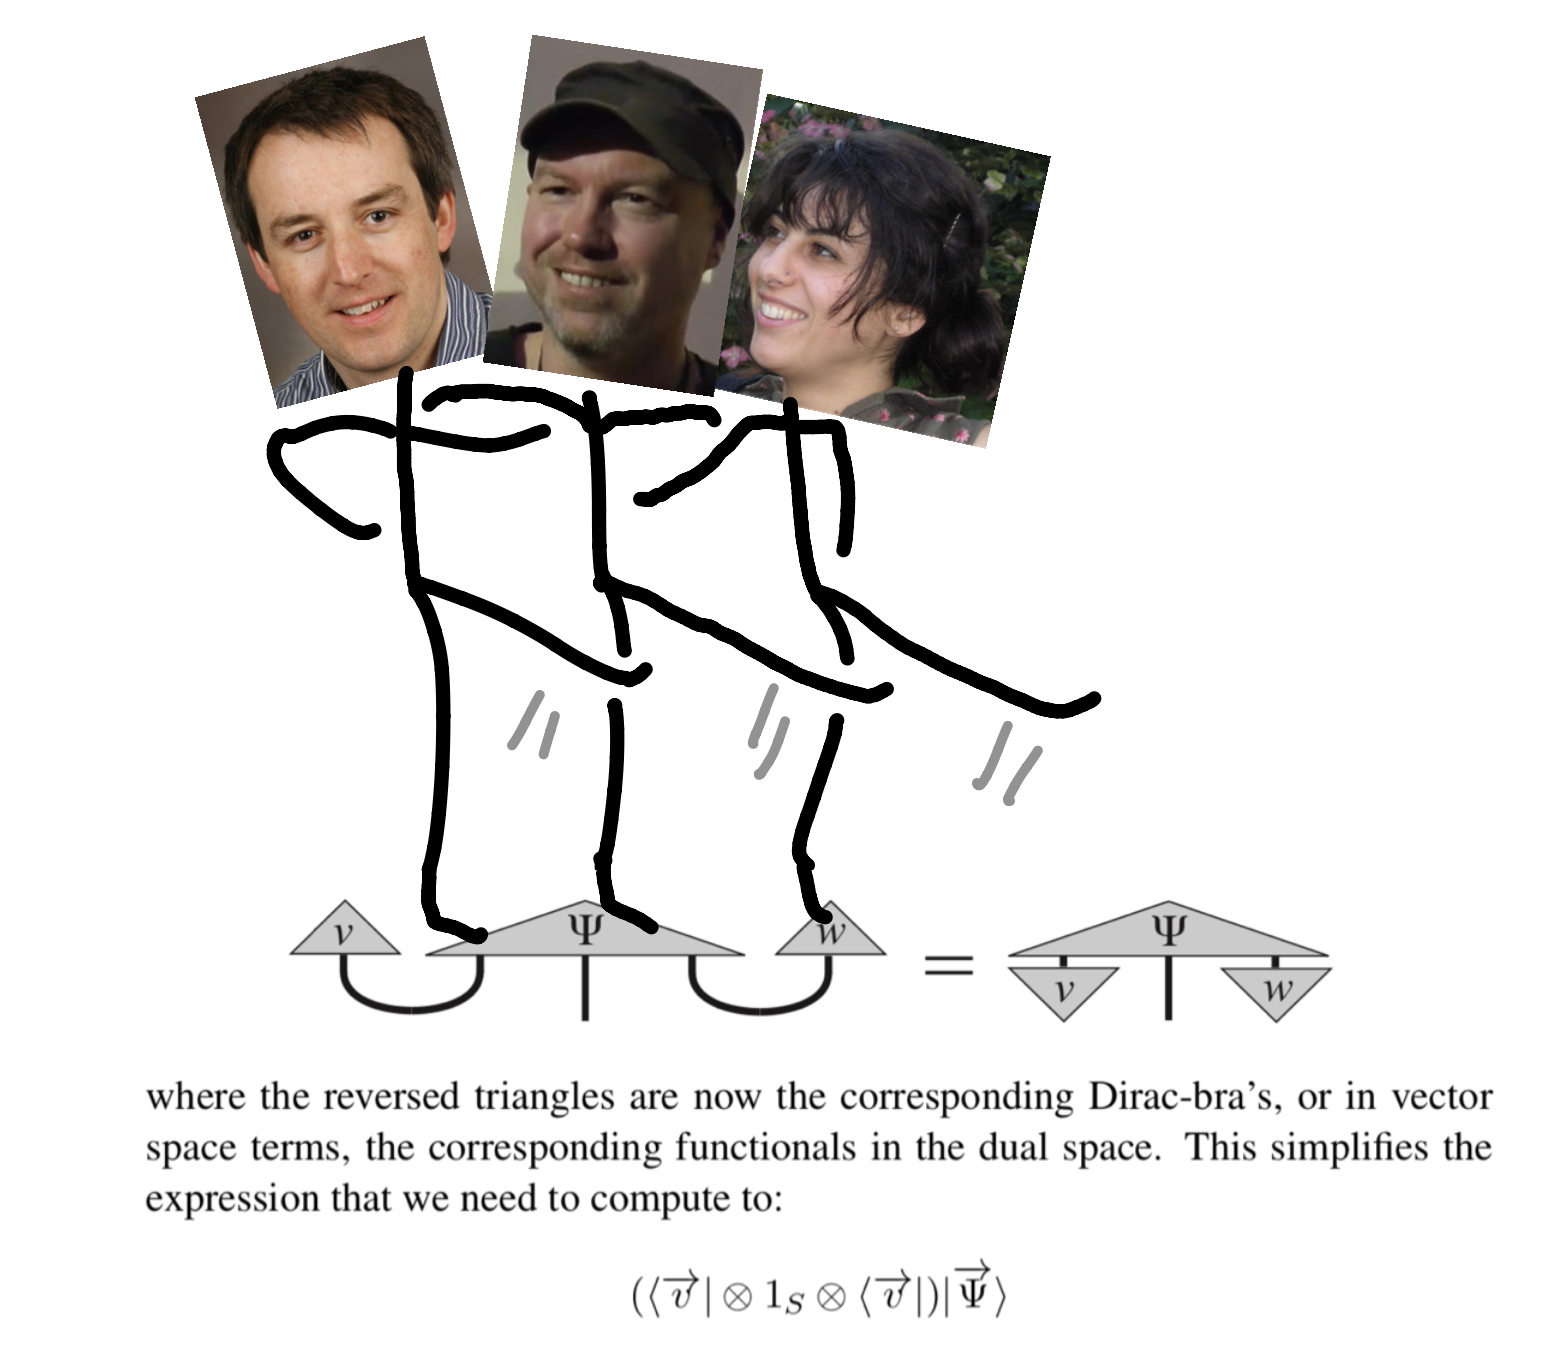
\includegraphics{figures/cartoons/disco1}}
\caption{Steve Clark was a professor in the computer science department at Oxford, and he was wondering how to compose vector-based semantic representations. Steve asked Bob, who realised suddenly what Jim was talking about. Mediated by the linguistic expertise of Mehrnoosh who was a postdoctoral researcher in Oxford at the time, pregroup diagrams were born. The basic types $n$ and $s$ are assigned finite-dimensional vector spaces, concatenation of types the kronecker product $\otimes$, and by the isomorphism of dual spaces in finite dimensions there is no need to keep track of the left- and right- inverse data. Words become vectors, and pregroup reductions become bell-states, or bell-measurements, depending on whether one reads top-down or bottom-up. There was simply no other game in town for an approach to computational linguistics that combined linguistic compositionality with distributional representations.}
\end{figure}

\begin{figure}[h!]
\centering
\scalebox{1}{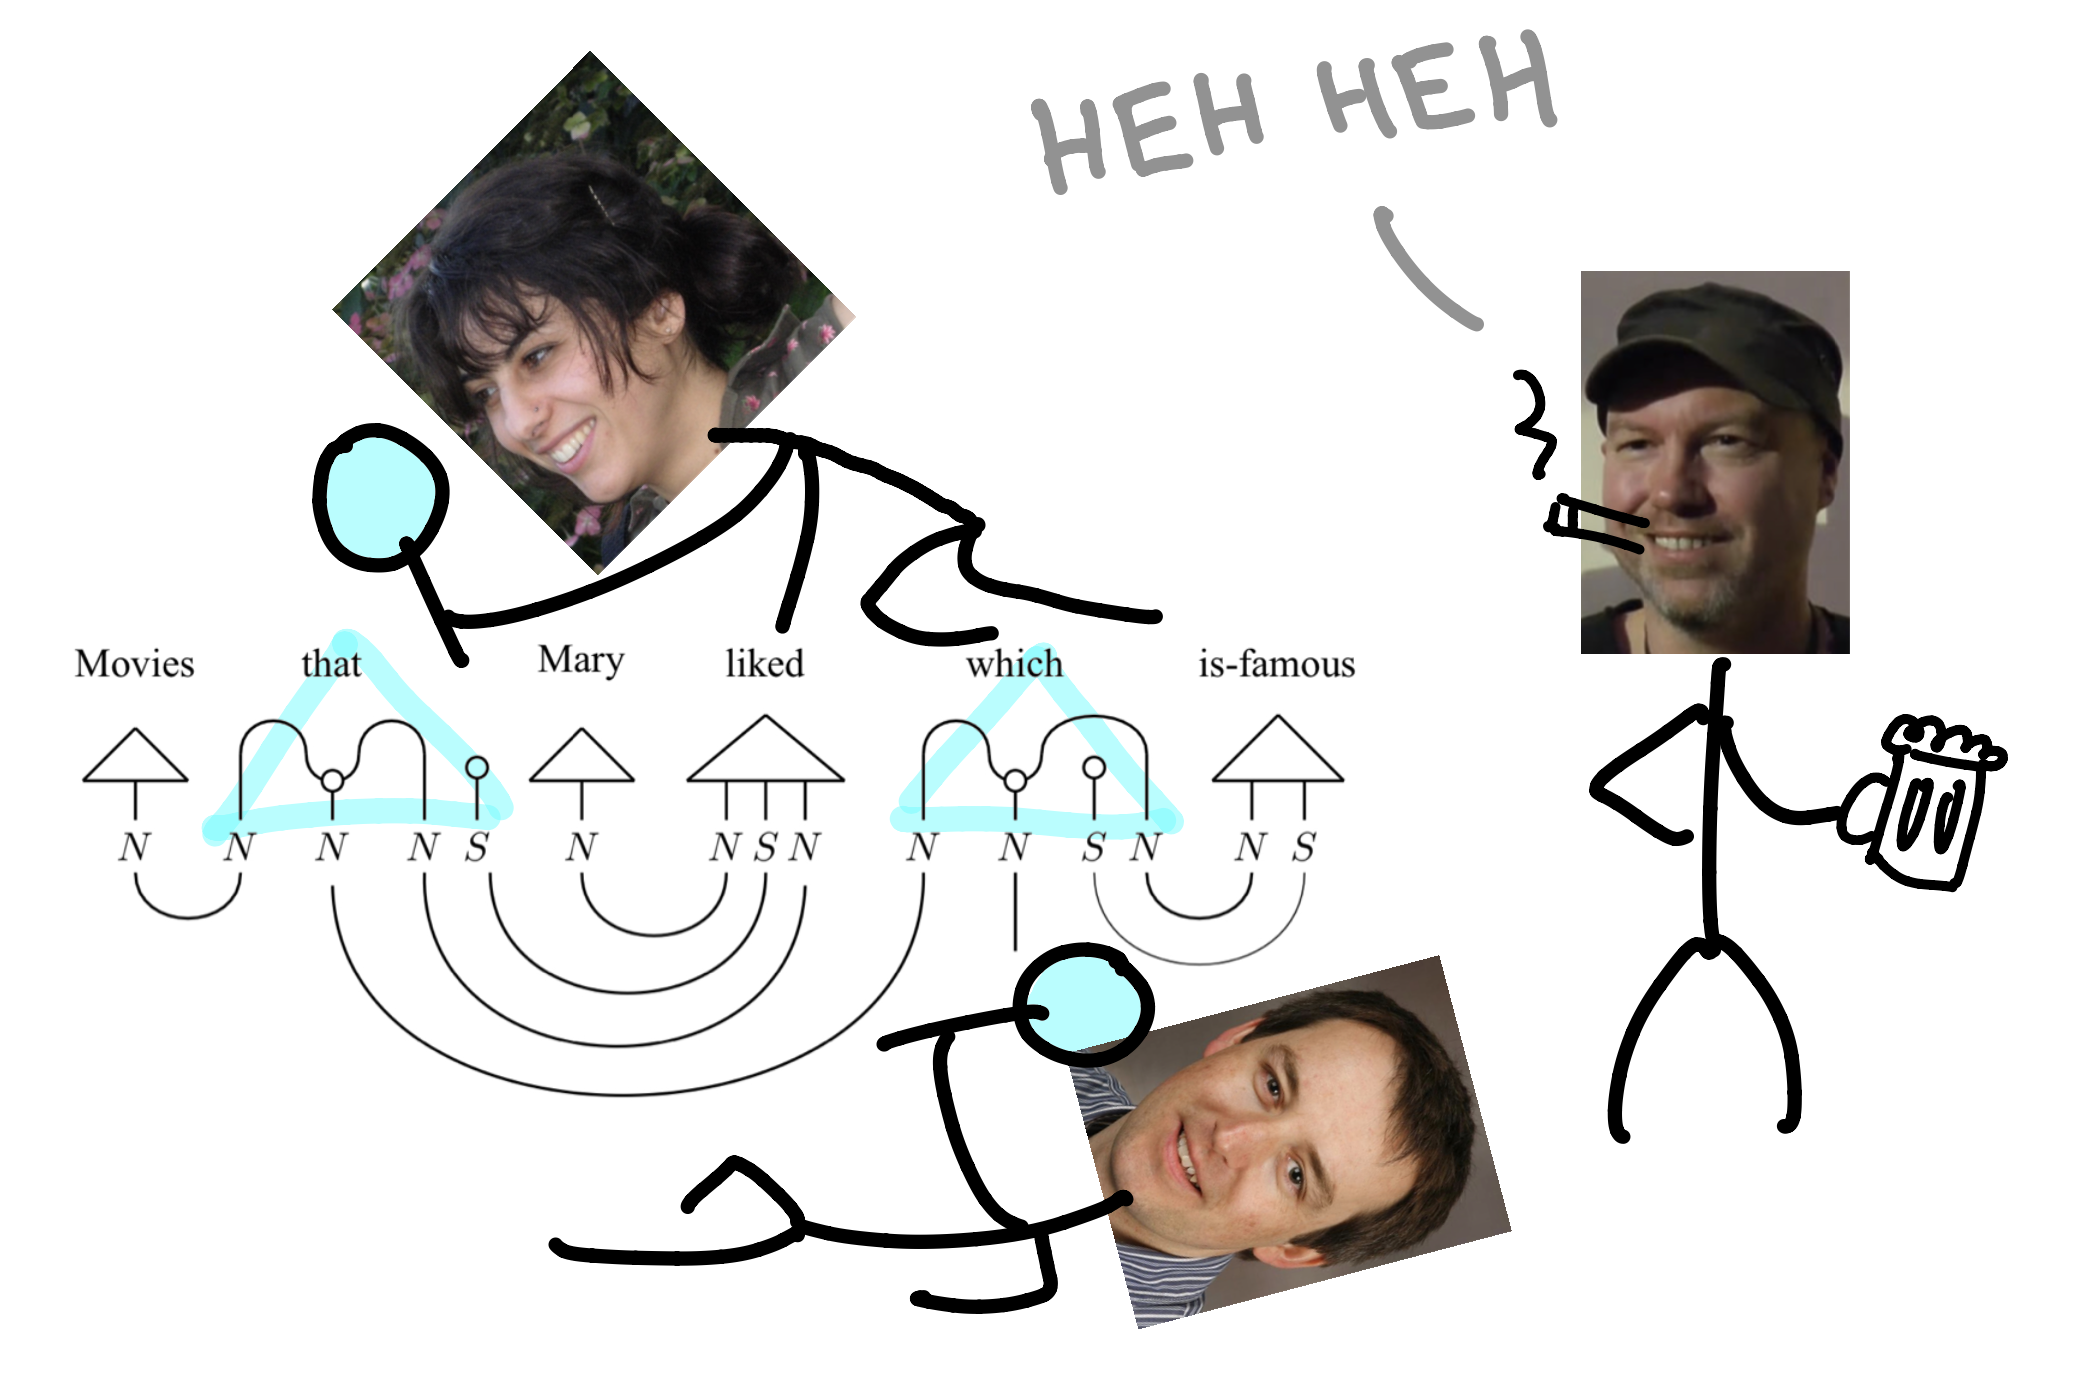
\includegraphics{figures/cartoons/disco2}}
\caption{In \emph{the frobenius anatomy of relative pronouns}\bR CITE \e, the trio realised that spiders could play the role of relative pronouns, which was genuinely novel linguistics. If one follows the noun-wire of "movies", one sees that by declaring the relative pronoun to be a vector made up of a particular bunch of spiders-as-multiwires, "movies" is copied to be related to the "liked" word, copied again by "which" to be related to the "is-famous" word, and a third time to act as the noun in the whole noun-phrase. This discovery clarified a value proposition: insights from quantum theory could be applied in the linguistic setting, and linguistics offered a novel use-case for quantum computers. For example, density matrices were used to model semantic ambiguity \bR CITE \e, and natural language experiments were performed on real quantum computeres \bR CITE \e.}
\end{figure}

\begin{figure}[h!]
\centering
\scalebox{1}{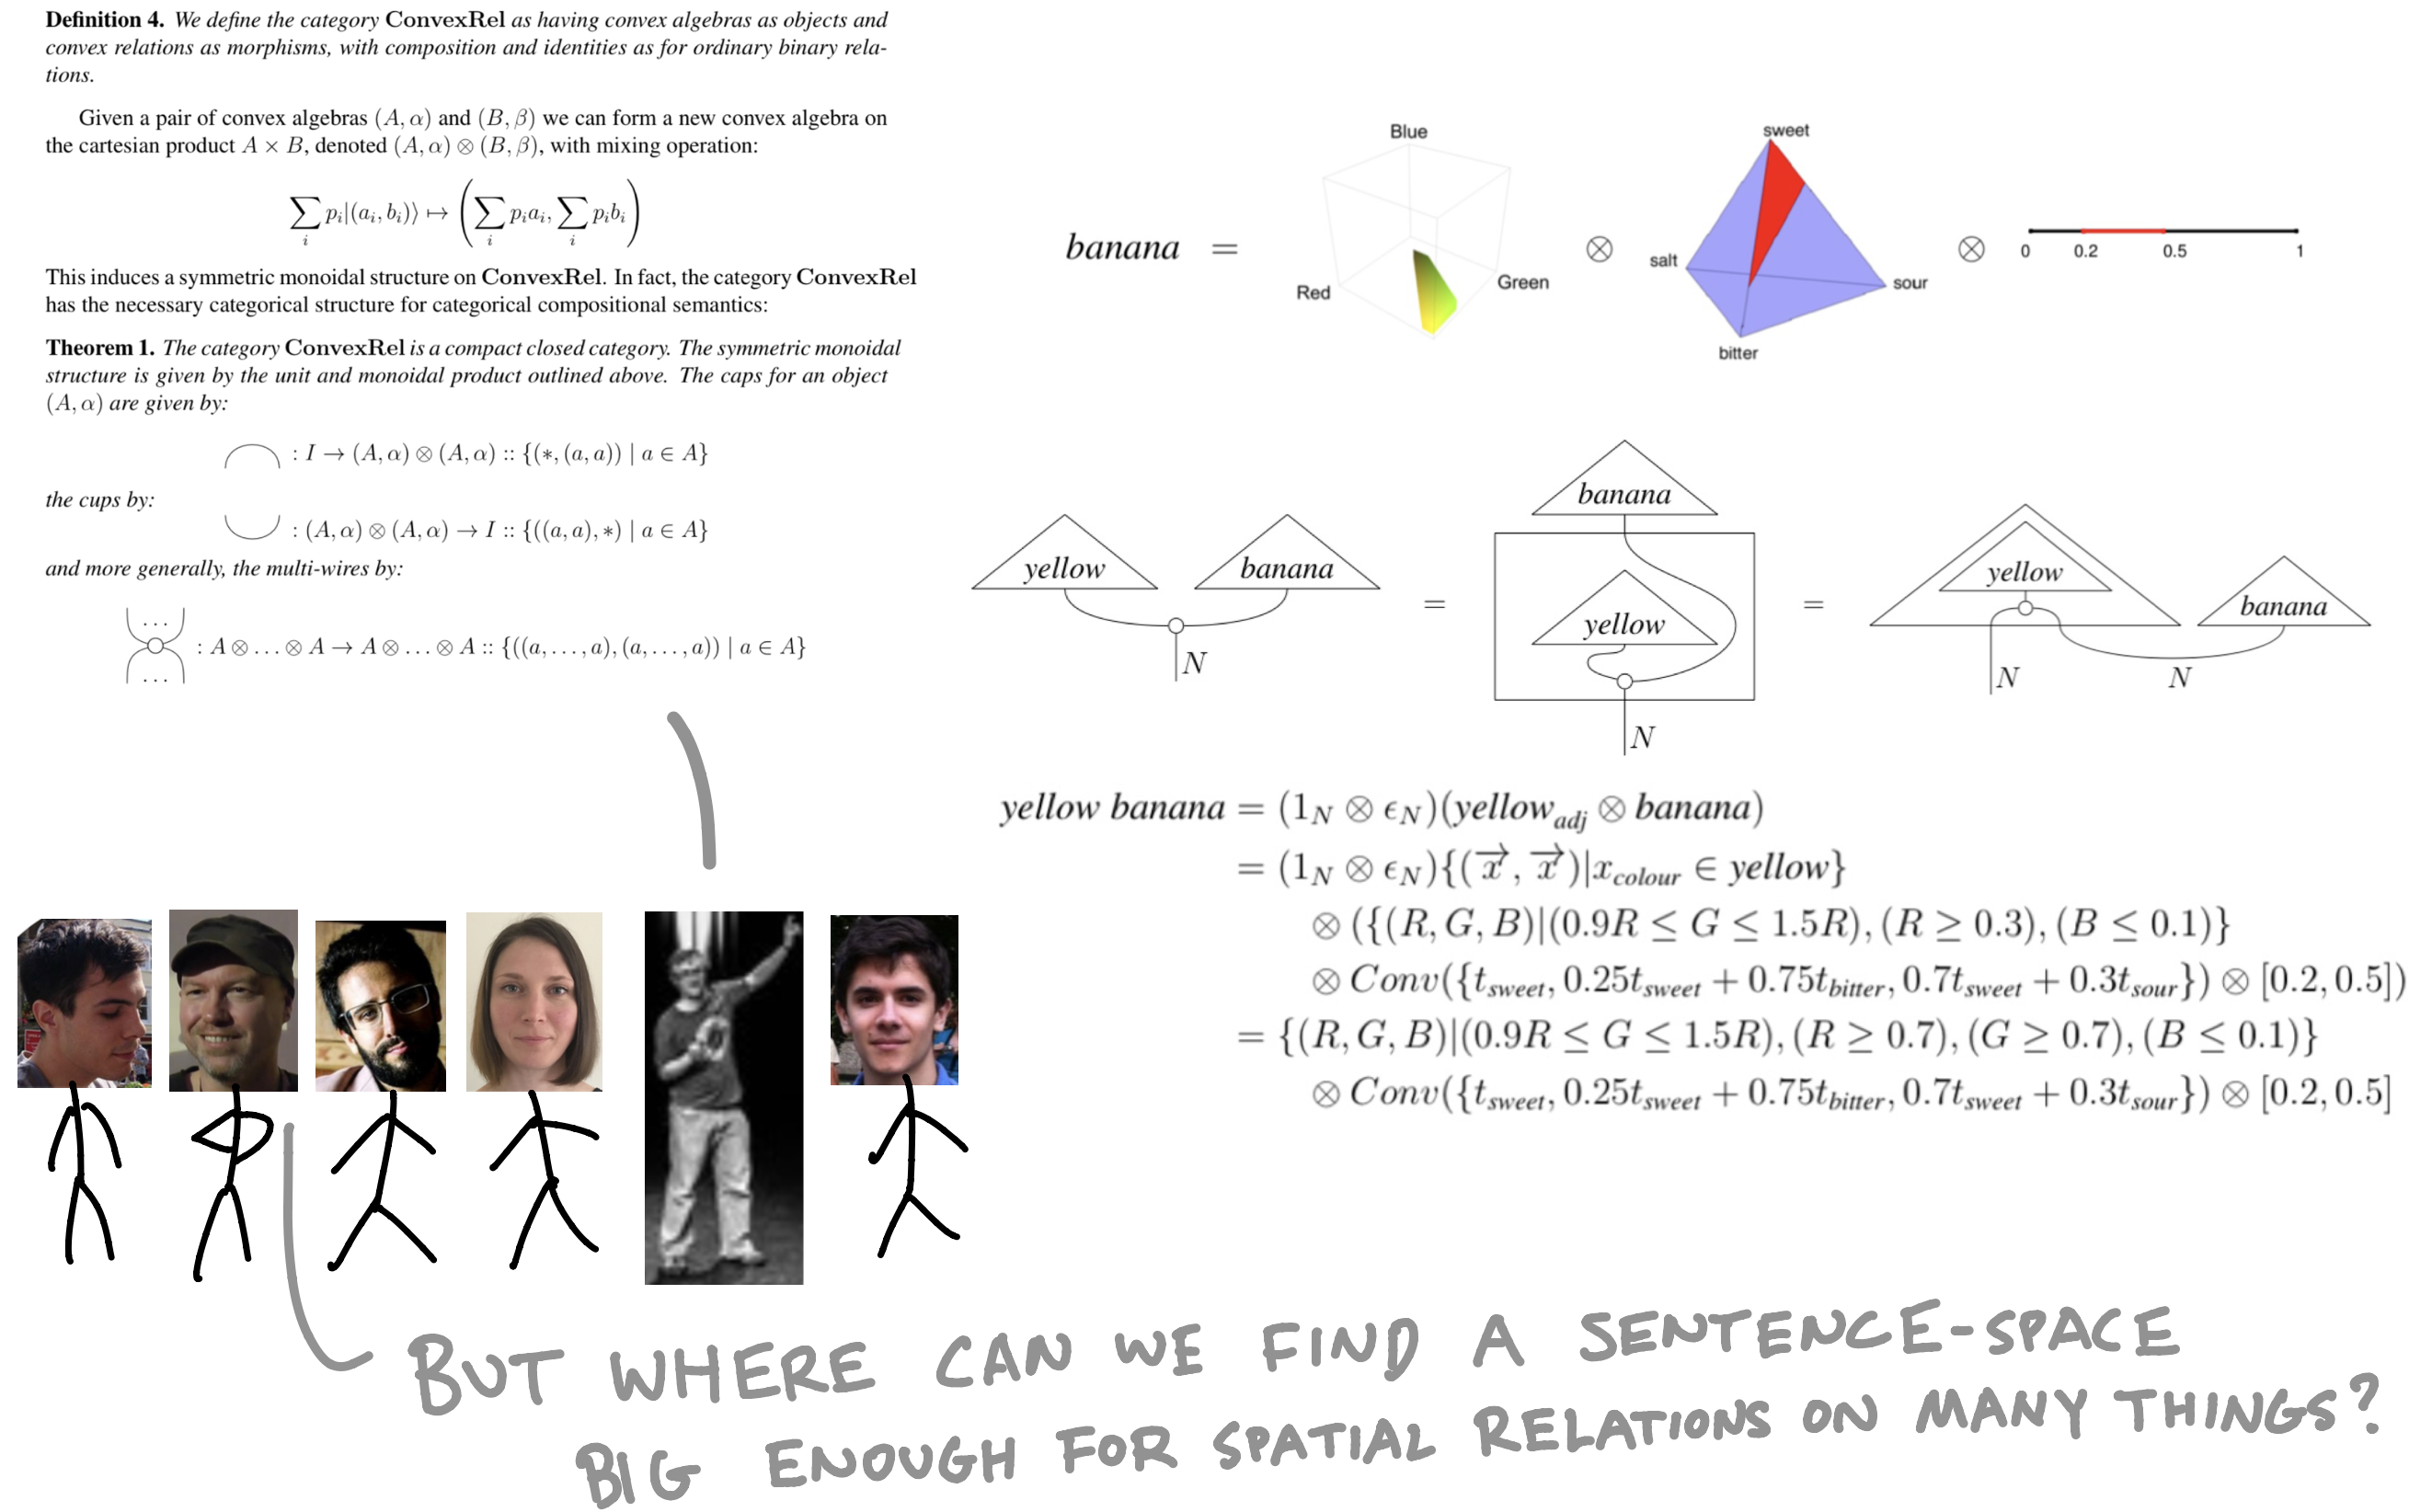
\includegraphics{figures/cartoons/disco3}}
\caption{Keeping the structure of the diagrams but seeking set-relational rather than vector-based semantics, a bridge was made between linguistics and cognitive science in \emph{interacting conceptual spaces I}\bR CITE \e. Briefly, G\"{a}rdenfors posits that spatial representations of concepts mediate raw sense data and symbolic representations -- e.g. red is a region in colourspace -- and moreover that concepts ought to be spatially convex -- e.g. mixing any two shades of red still gives red. This paper created a new point in the value proposition: that new mathematics would arise from investigating the linguistic-quantum bridge, e.g. generalised relations \bR CITE \e. Although labelled as if it is the first in a series, the paper never saw a sequel by the same title, blocked by an apparently simple but actually tricky theoretical problem. The problem is that while this convex-relational story worked for conceptual adjectives modifying a single noun such for "sweet yellow bananas", there was difficulty in extending the story to work for multiple objects interacting in the same space, as in "cup on table in room". It couldn't be worked out what structure a sentence-wire in \textbf{ConvexRel} ought to have in order to accommodate (in principle) arbitrarily many objects and spatial relations between them.\\

DisCoCat then diverges from the story I want to tell. In no particular order, QNLP was done on an actual quantum computer \bR CITE \e, some software packages were written \bR CITE \e, and some art was made \bR CITE \e.}
\end{figure}
\clearpage



\subsection{I killed DisCoCat, and I would do it again.}

\begin{figure}[h!]
\centering
\scalebox{1}{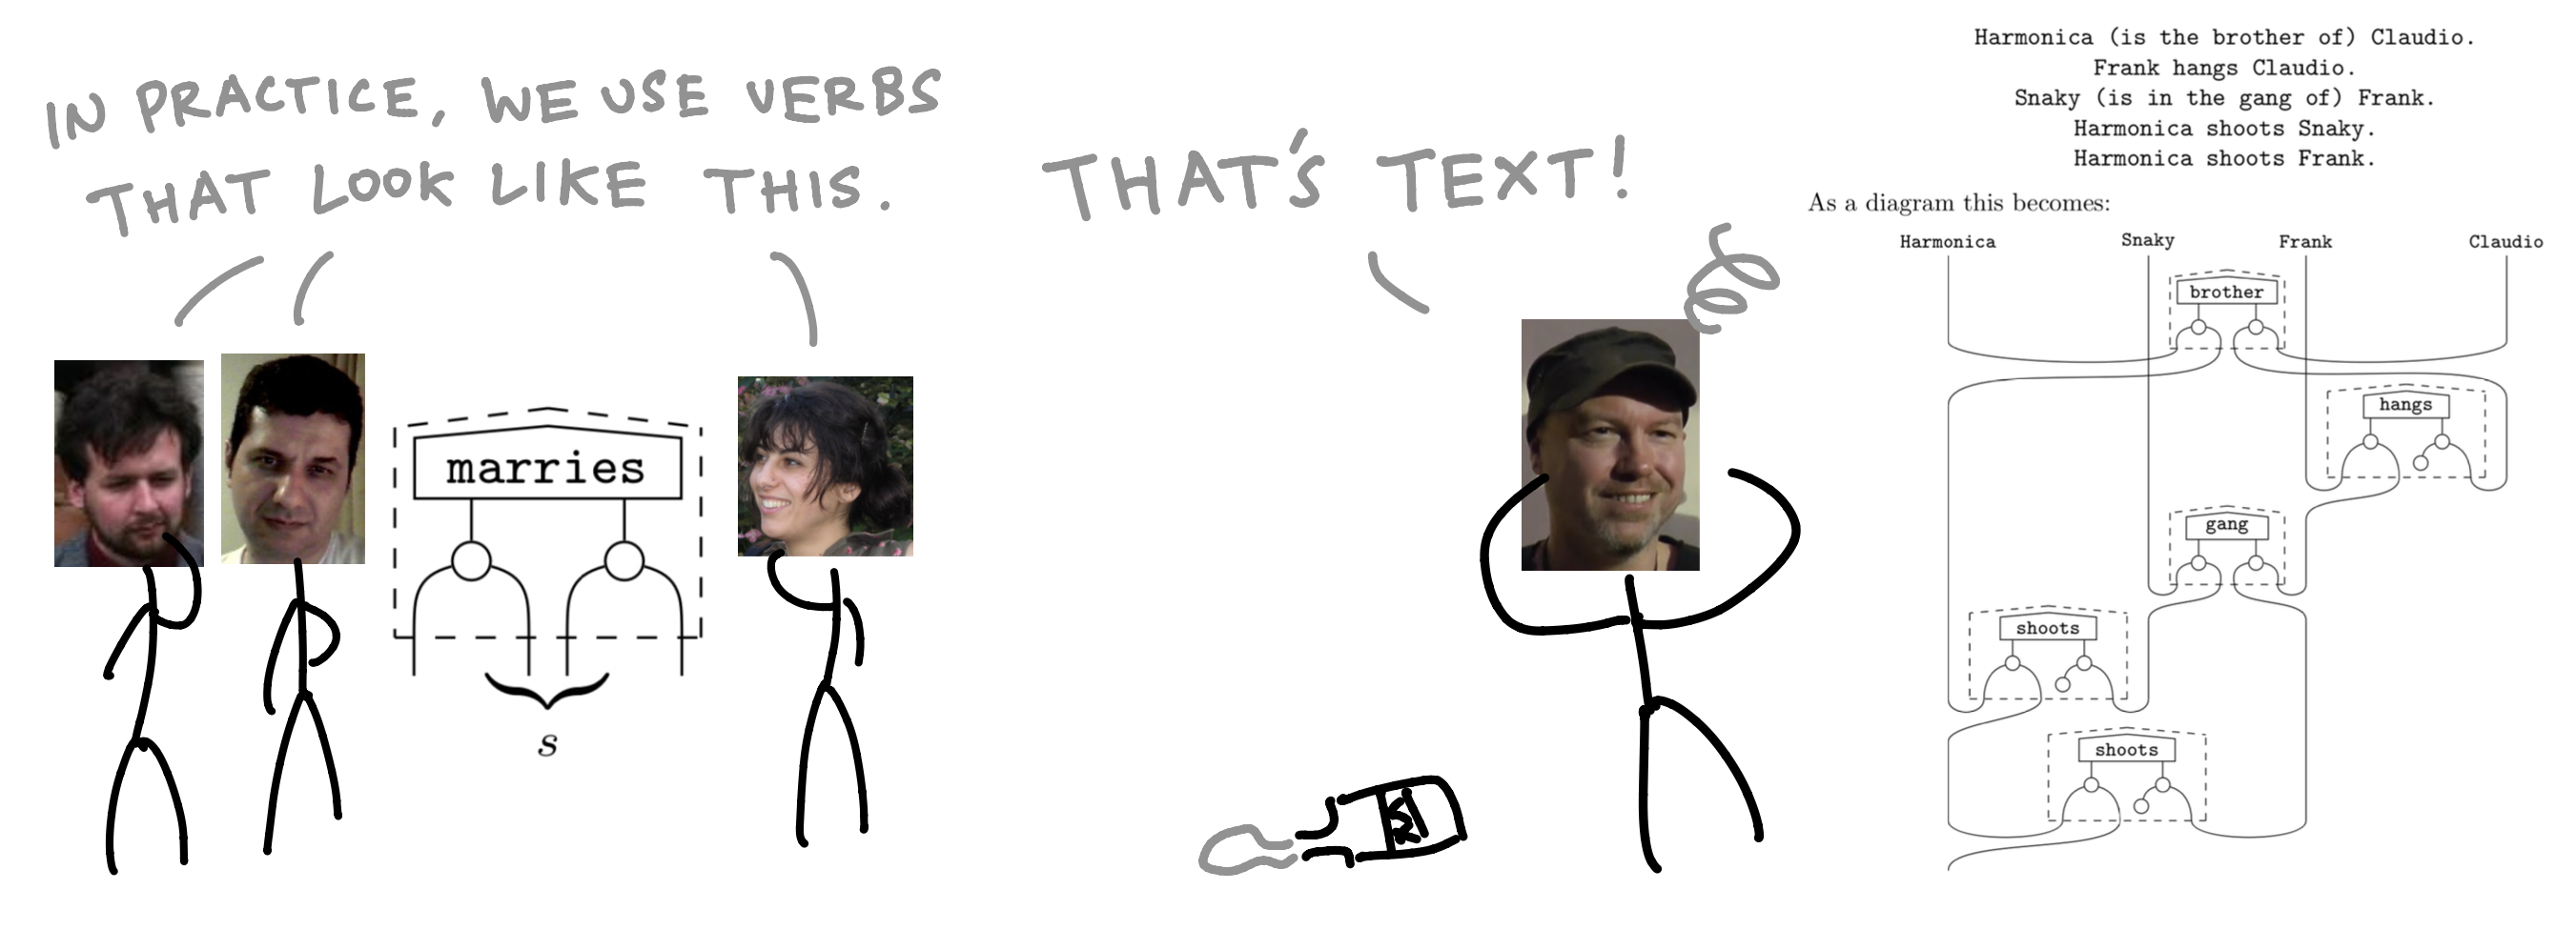
\includegraphics{figures/cartoons/discocirc1}}
\caption{It is a common evolutionary step in linguistics that theories `break the sentential barrier', moving from sentence-restricted to text- or discourse-level analysis \bR CITE \e. The same thing happened with DisCoCirc, due to a combination of practical constraints and theoretical ambition. On the practical side, wide tensors were (and remain) prohibitively expensive to simulate classically and actual quantum computers did not (and still do not) have many qubits, hence in practice pregroup diagrams were reduced to thinner and deeper circuits, often with the help of an additional simplifying assumption that sentence wires were pairs of noun wires in the illustrated form on the left. Theoretically, seeking dynamic epistemic logic, Bob had an epiphanous hangover (really) where he envisioned that these "Cartesian verbs" could be used in service of compositional text meanings, and he called this idea DisCoCirc \bR CITE \e.}
\end{figure}

\begin{figure}[h!]
\centering
\scalebox{1}{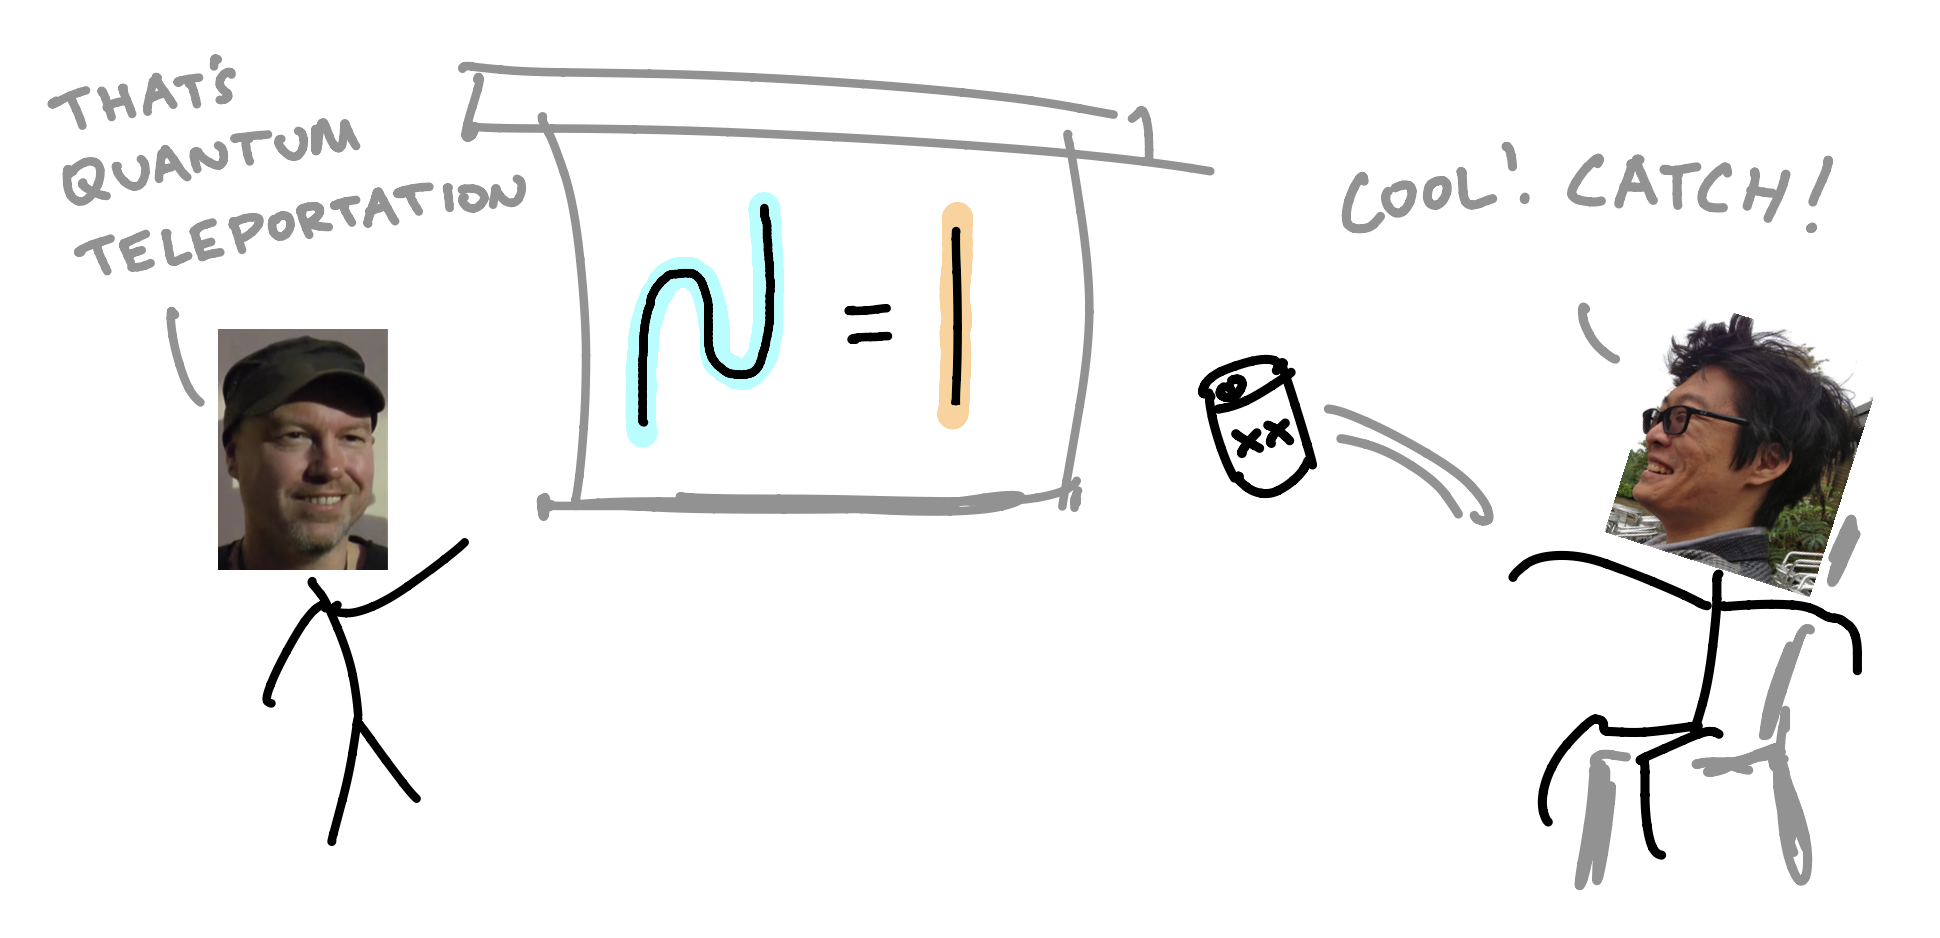
\includegraphics{figures/cartoons/v1}}
\caption{I met Bob in my master's in 2019, where he taught the picturing quantum processes course. When quantum teleportation was explained in half a minute by a diagram, I decided to pursue a DPhil in diagrammatic mathematics. In the last lecture, I threw Bob a cider, after which he seemed to like me. I did not know he was an alcoholic.}
\end{figure}
\clearpage

I was shanghaied into thinking about diagrams for language. I was deeply dissatisfied with the content from the standpoint my own intellectual integrity. Firstly, there seemed to me an unspoken claim that the presence of cups in pregroup diagrams (which implied a noncartesian and hence large tensor product) made it necessary to use quantum computers to effectively compute pregroup diagrams. I just could not believe that my brain required quantum computation to understand language. This implicit claim of kinship between quantum and linguistics was further entrenched by the analysis of the relative pronoun in terms of frobenius algebras, since spiders in $\mathbf{Vect}^\otimes$ were the \emph{sine qua non} of categorical quantum mechanics. The best steelman for spiders I have is that frobenius algebras (which are central to bicategories of relations \bR CITE \e) just happen to be a ubiquitous mathematical structure that are well-suited to express the mathematics of connections, both in language and in quantum.\\

Second, representing the content of a sentence as a vector in a sentence-vector-space did not sit well with me, since this move meant that the only meaningful thing one could do with two sentences was take their inner-product as a measure of similarity. Moreover, I had the theoretical concern that language is in principle indefinitely productive, so one could construct a sentence that marshalled indefinitely many nouns, and at some point for any finite vector space $s$ one would run out of room to encode relationships, or else they would be cramped together in a way that did not suit intuitions about the freedom of constructing meanings using language. I always believed in the existence of a simple, practical, and intuitive categorical, compositional, and distributional semantics; I just didn't believe that the role of quantum -- however helpful or interesting -- was \emph{necessary}.

My first unsatisfactory attempt was in my Master's thesis \bR CITE \e. It had been known for a while that a free autonomous category construction by Delpeuch \bR CITE \e could potentially eliminate some of the cups in pregroup diagrams, yielding what amounted to a method to transform a pregroup diagram into a monoidal string diagram in the shape of a context-free grammar tree. This trick had the limitation that freely adding directed cups and caps to a string diagrammatic signature did not turn a symmetric monoidal category into a (weakly) compact closed one, rather just into a monoidal category where the original wires had braidings, but all the new left and right dual wires did not; this presented difficulties in accounting for iterated duals for higher-order modifiers such as adverbs in grammatical types, and had nothing to say about spiders. I tried to generalise this trick to `freely' adding arbitrary diagrammatic gadgets to string diagrams, but my assessor Samson pointed out that it was nontrivial to determine whether such constructions were faithful. In retrospect the free autonomous completion of a parameterised \bR CITE \e markov category \bR CITE \e is in the ballpark of dequantumfying pregroup diagrams, but I didn't learn about them until later, and that still wouldn't have addressed the issues that come with only having a sentence-wire.

\begin{figure}[h!]
\centering
\scalebox{1}{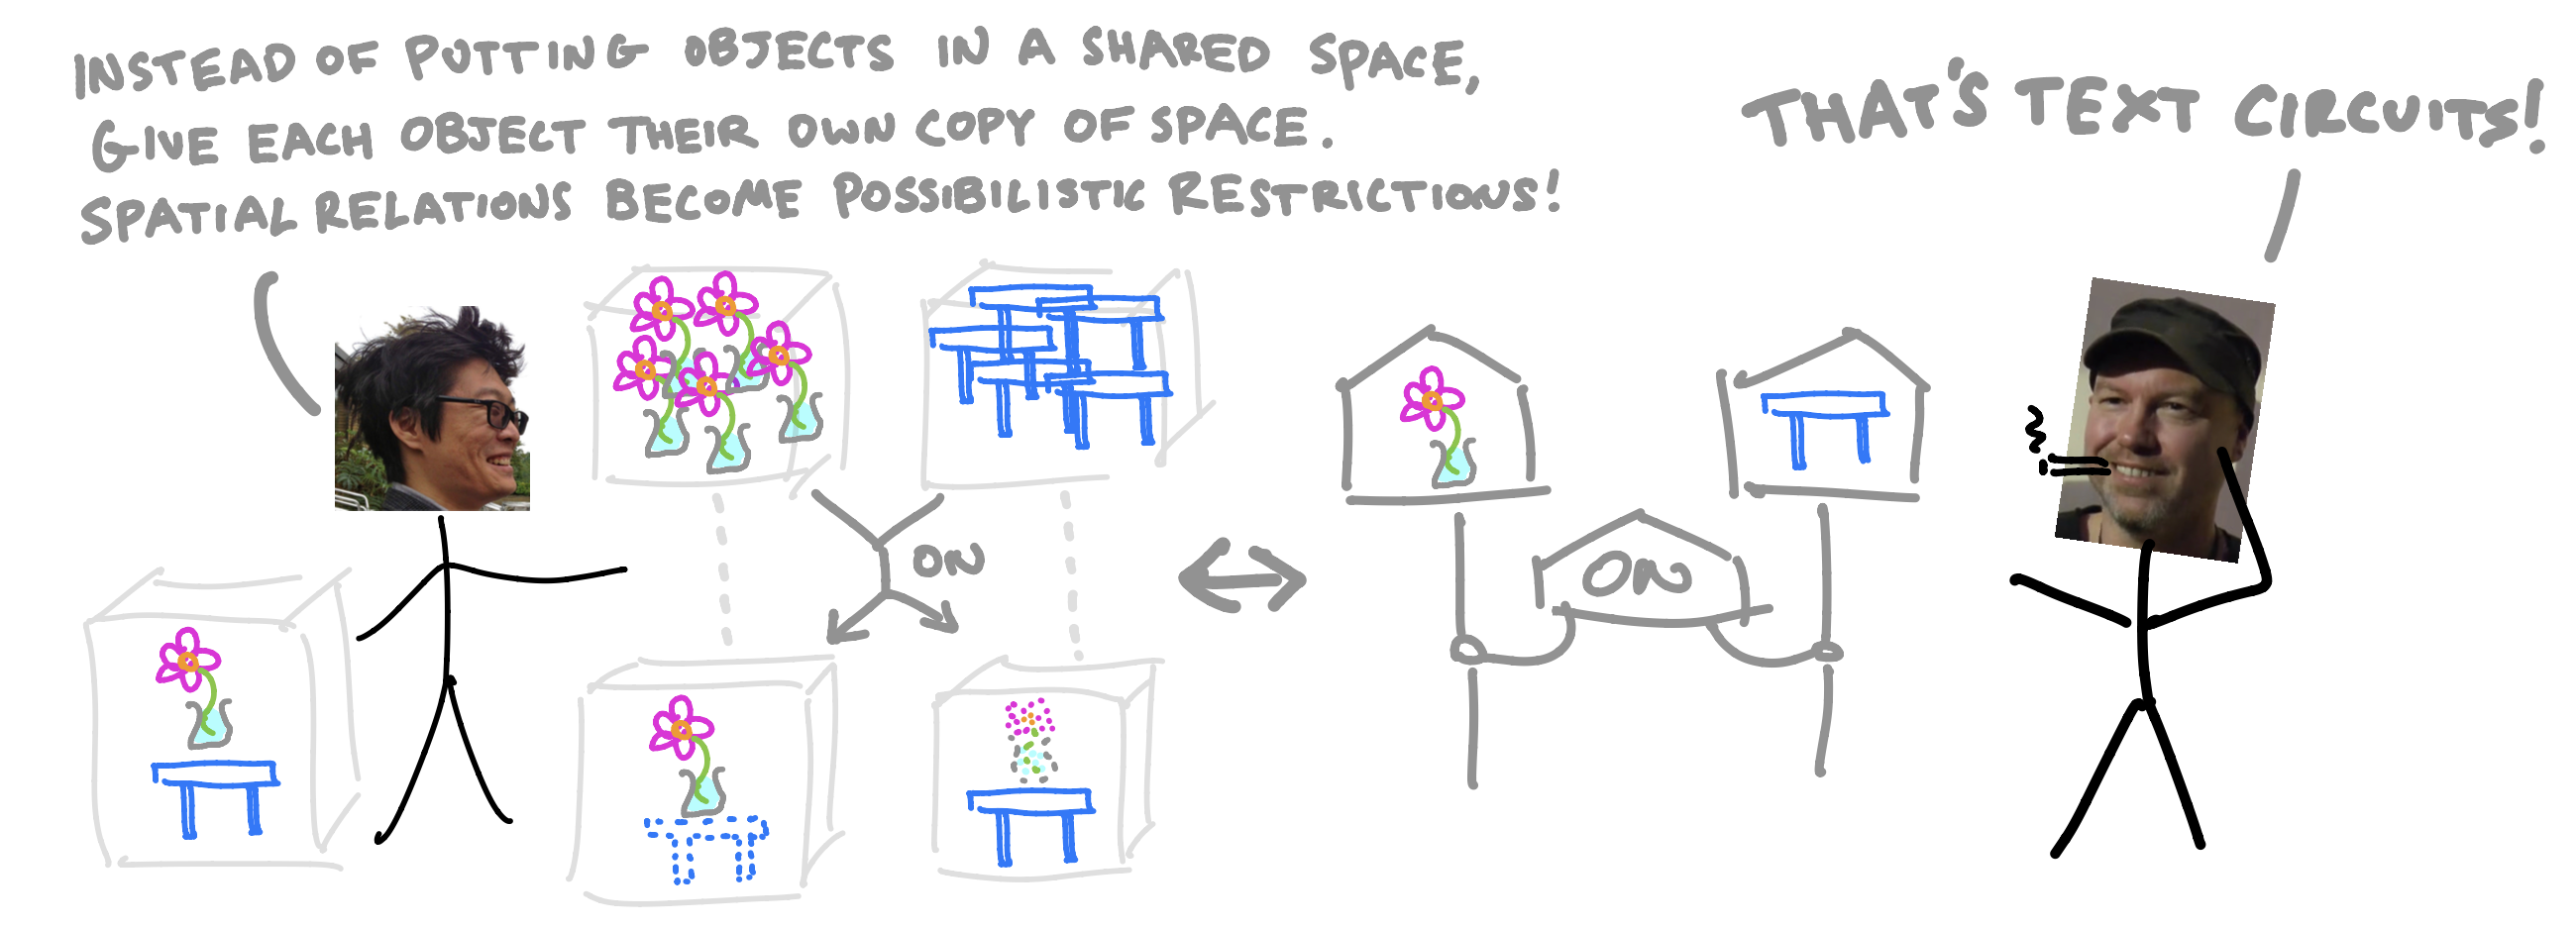
\includegraphics{figures/cartoons/circify1}}
\caption{Then COVID happened. During the first lockdown, I visited Bob's garden under technically legal circumstances, and I suggested a solution to the longstanding problem of representing linguistic spatial relationships. My theoretical concern was the culprit: the initial attempts at the problem failed because the approach was to find a single sentence object $s$ in which one could paste the data of arbitrarily many distinct spatial entities. The simple solution was a change in perspective.}
\end{figure}

\begin{figure}[h!]
\centering
\scalebox{1}{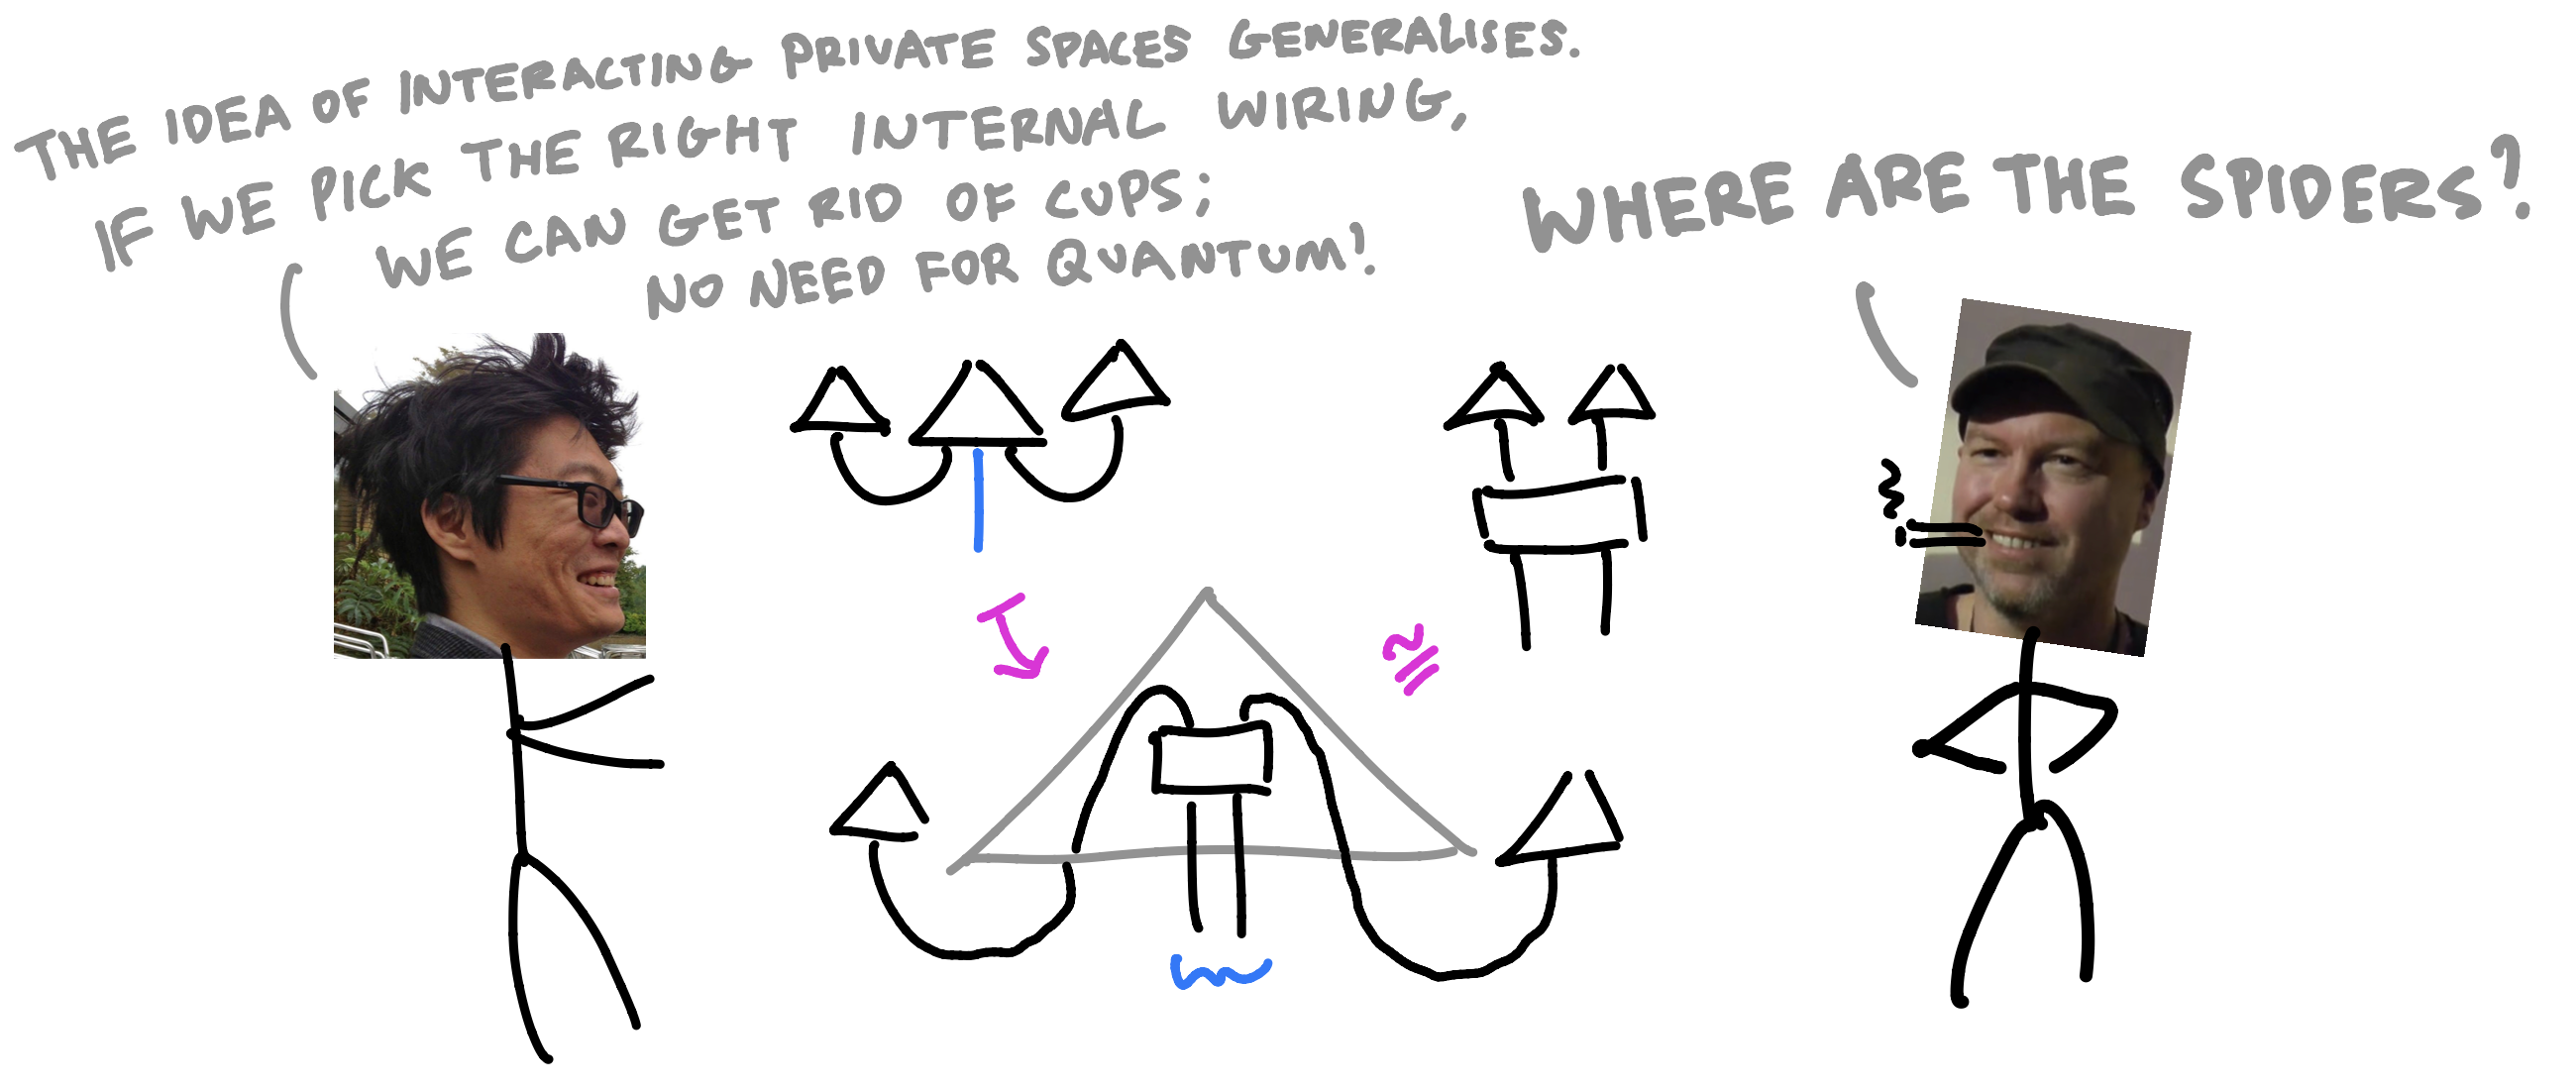
\includegraphics{figures/cartoons/circify2}}
\caption{That this move of splitting up the sentence-wire into a sentence-dependent collection of wires was sufficient to solve what had appeared to be a difficult problem prompted some re-examination of foundations. The free autonomisation trick in conjunction with sentence-wire-as-tensored-nouns seemed promising, but it became clear that right way to drown a DisCoCat thoroughly was to explain and eliminate the spiders.}
\end{figure}

\begin{figure}[h!]
\centering
\scalebox{1}{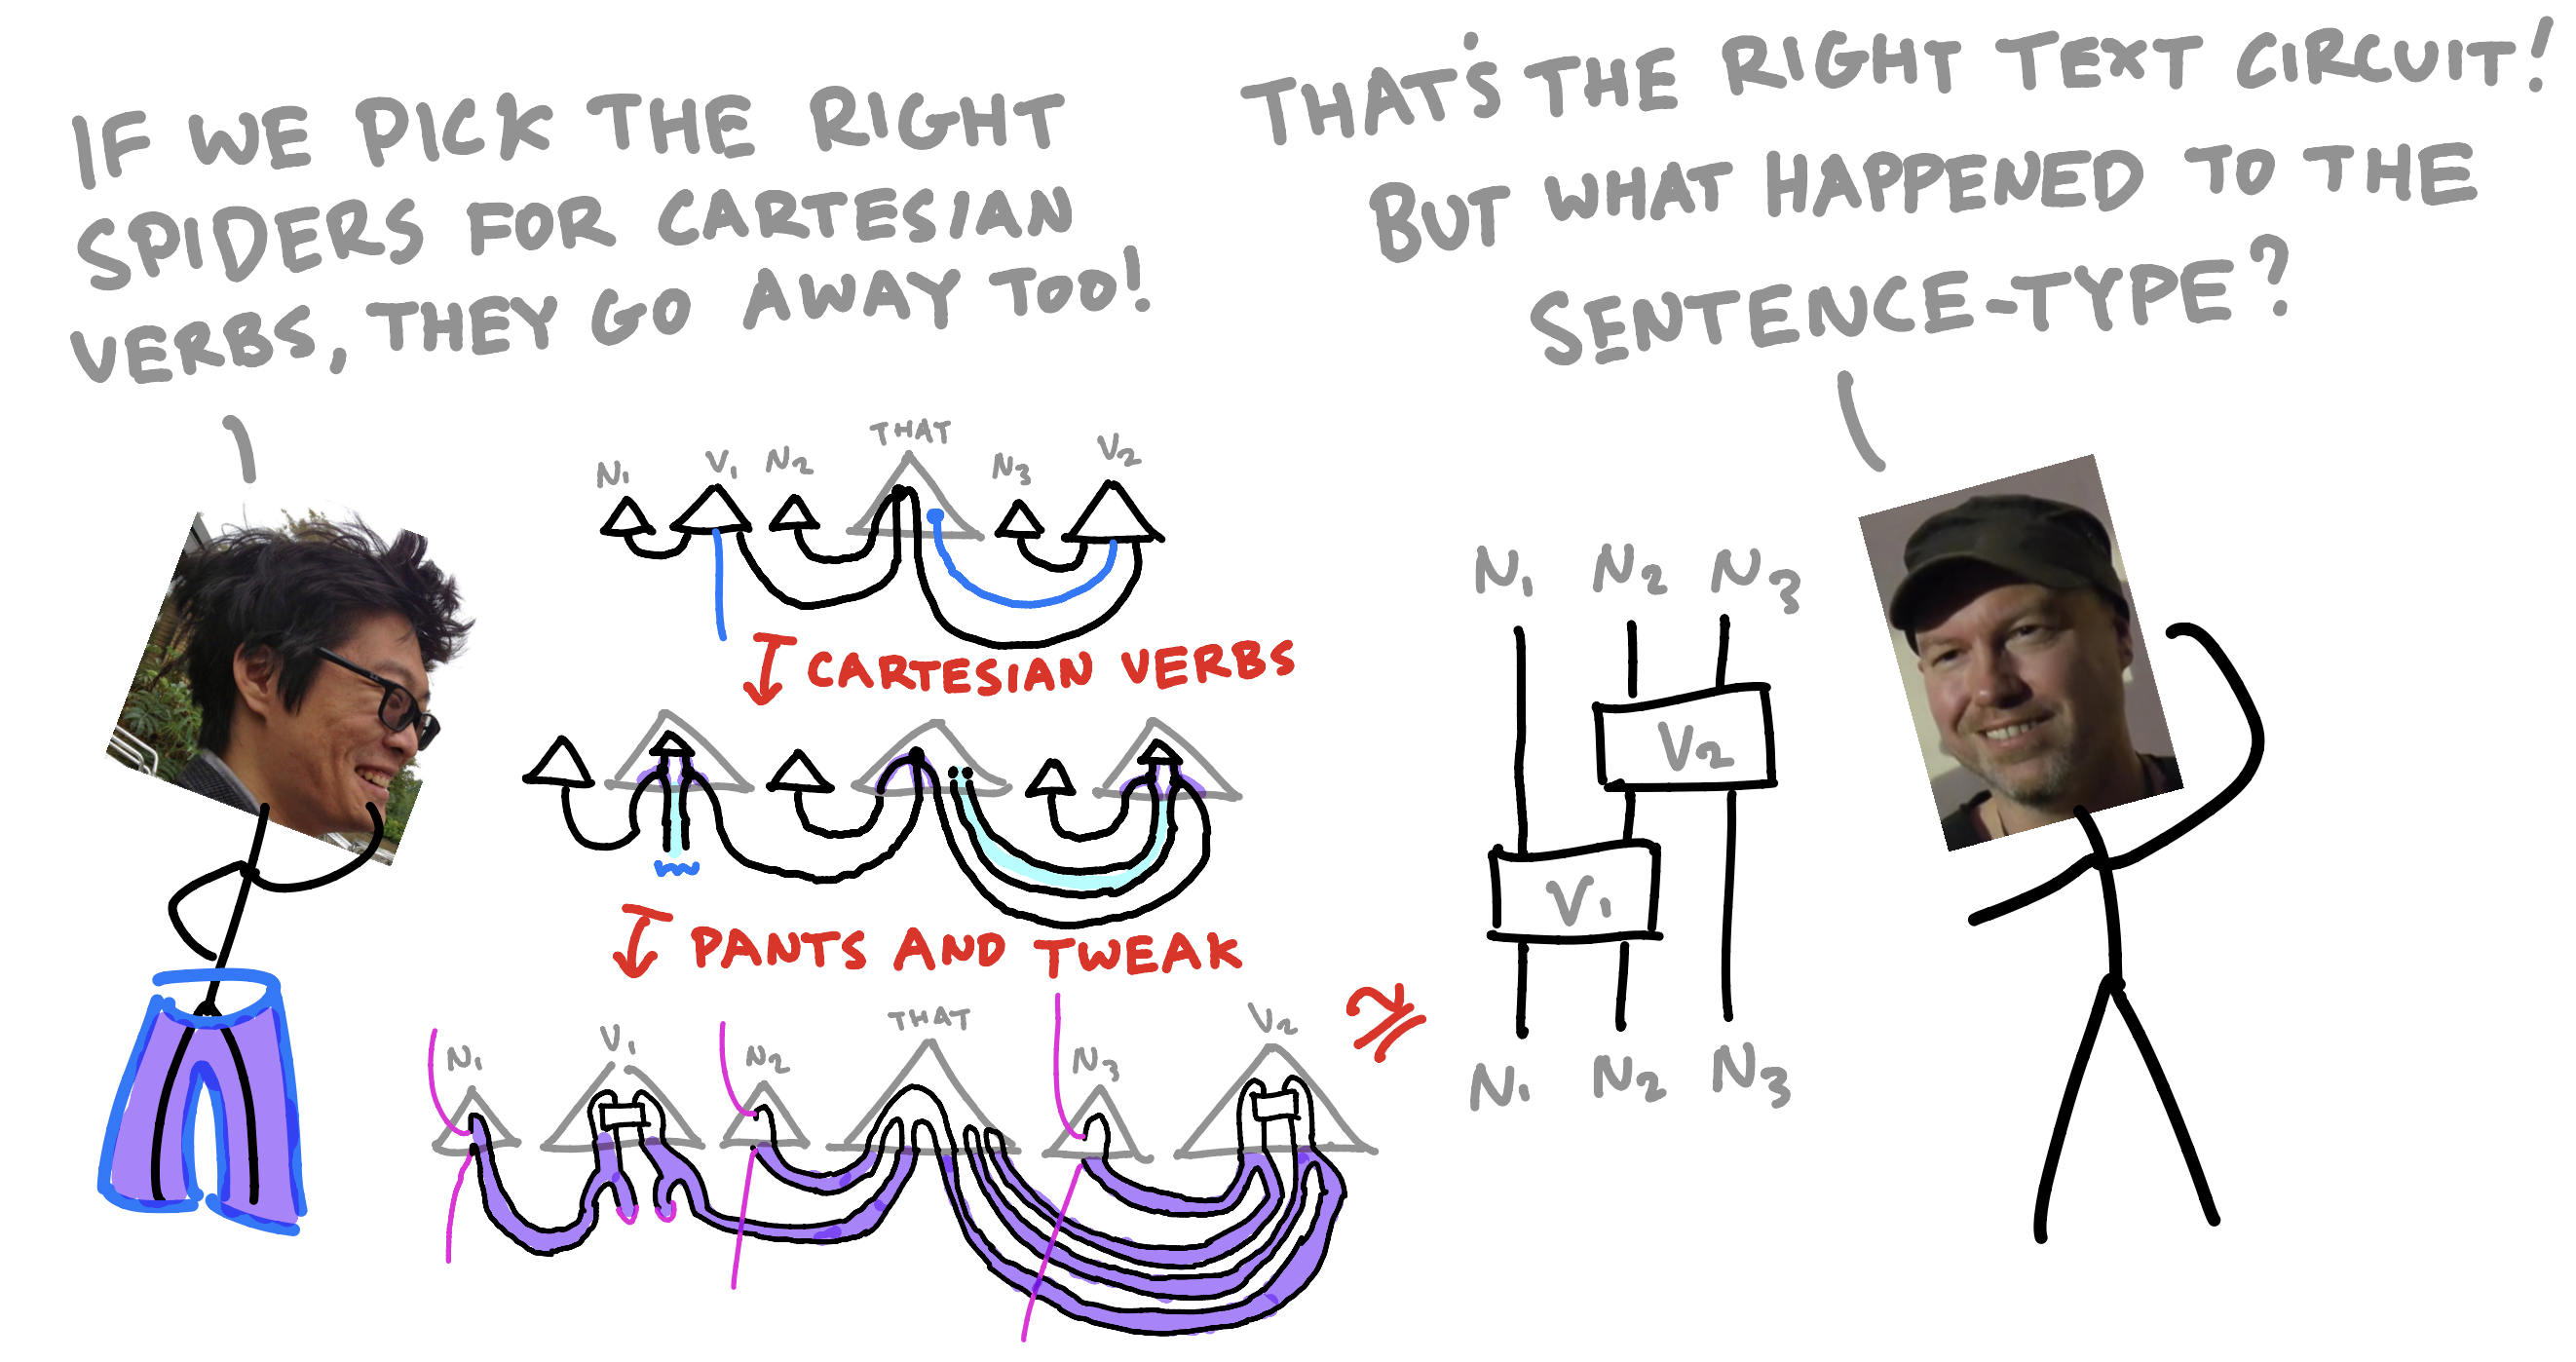
\includegraphics{figures/cartoons/circify3}}
\caption{I then discovered that by interpreting spiders as the well-known "pair of pants" algebra in a compact closed monoidal setting allowed for a procedure in which the final form was purely symmetric monoidal -- the absence of cups and caps meant that there was no practical necessity to interpret diagrams on quantum computers: \emph{any} computer would suffice. The role of spiders for relative pronouns was illuminated in the presence of splitting the sentence wire: the pair-of-pants are the algebra of morphism composition, and splitting the sentence wire into a collection of nouns allowed relative-pronoun-spiders to pick out the participating nouns to compose relationships onto.}
\end{figure}

\begin{figure}[h!]
\centering
\scalebox{1}{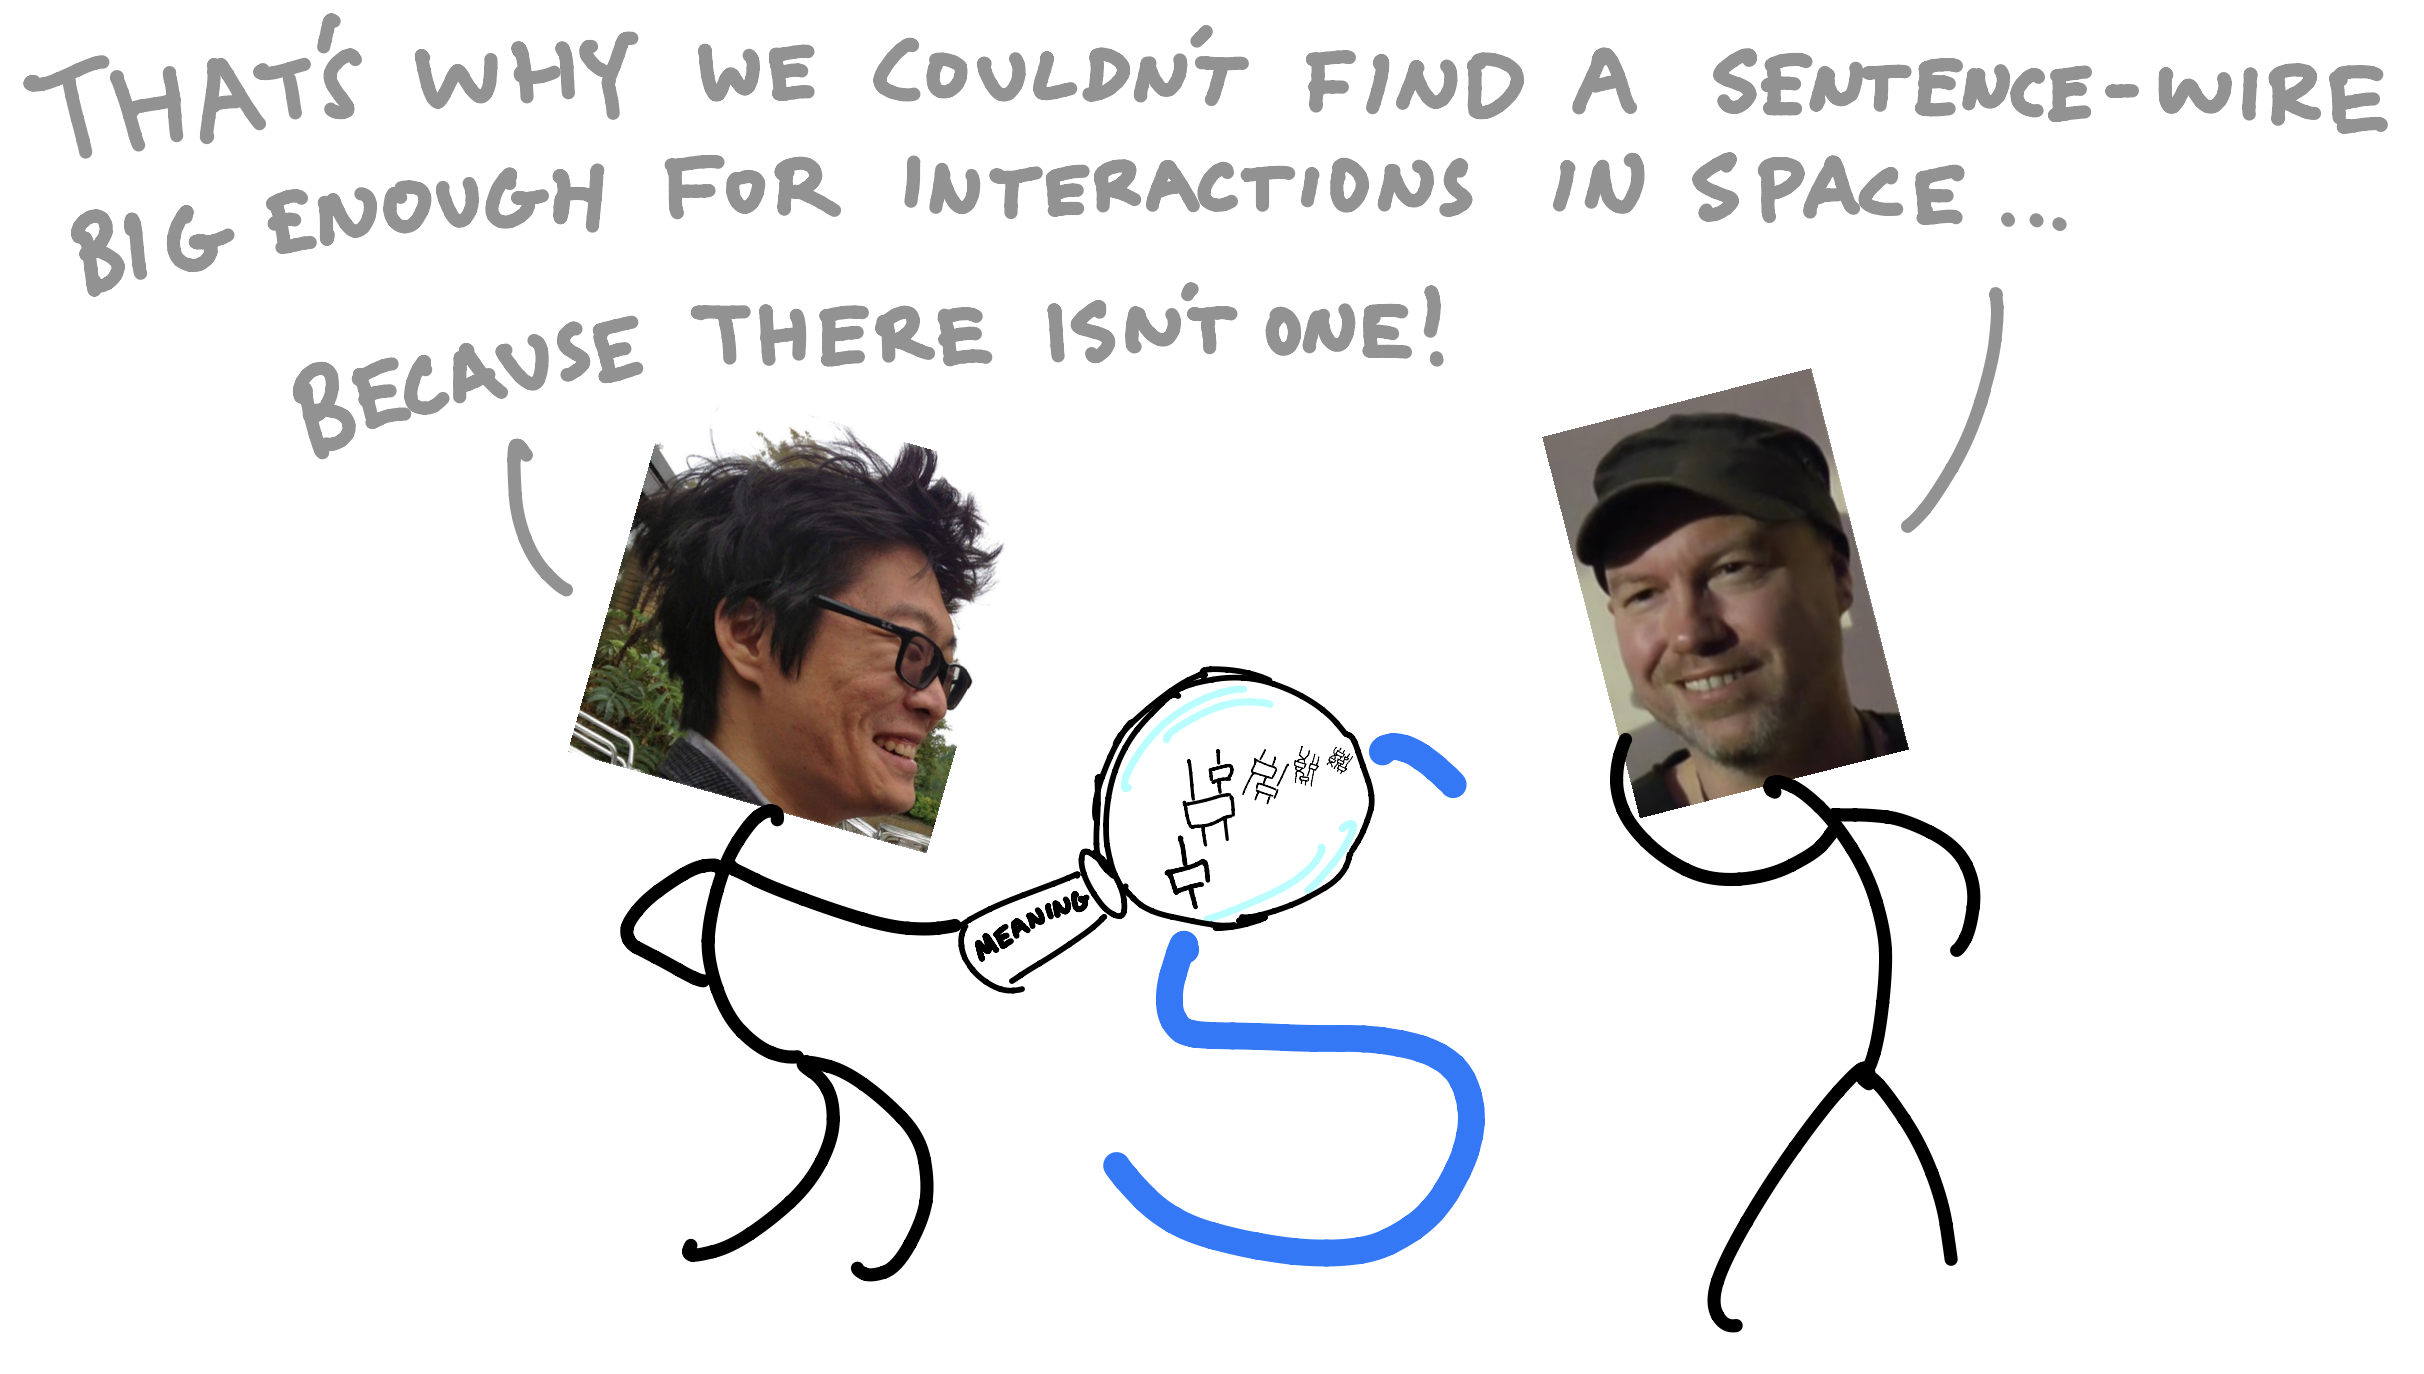
\includegraphics{figures/cartoons/nosent}}
\caption{A coherent conservative generalisation of DisCoCat with less baggage had emerged, or rather, DisCoCirc was placed to formally subsume DisCoCat. It was now understood that the sentence type was a formal syntactic ansatz for the sake of grammar, which was to be interpreted in the semantic domain not as a single wire, but as a sentence-dependent collection of wires. It was further realised that the complexity of pregroup diagrams was due to grammar -- the topological deformation of semantic connections to fit the one-dimensional line of language -- whereas the essential connective content of language could be expressed in a simple form that distilled away the bureaucracy of syntax.}
\end{figure}

\begin{figure}[h!]
\centering
\scalebox{1}{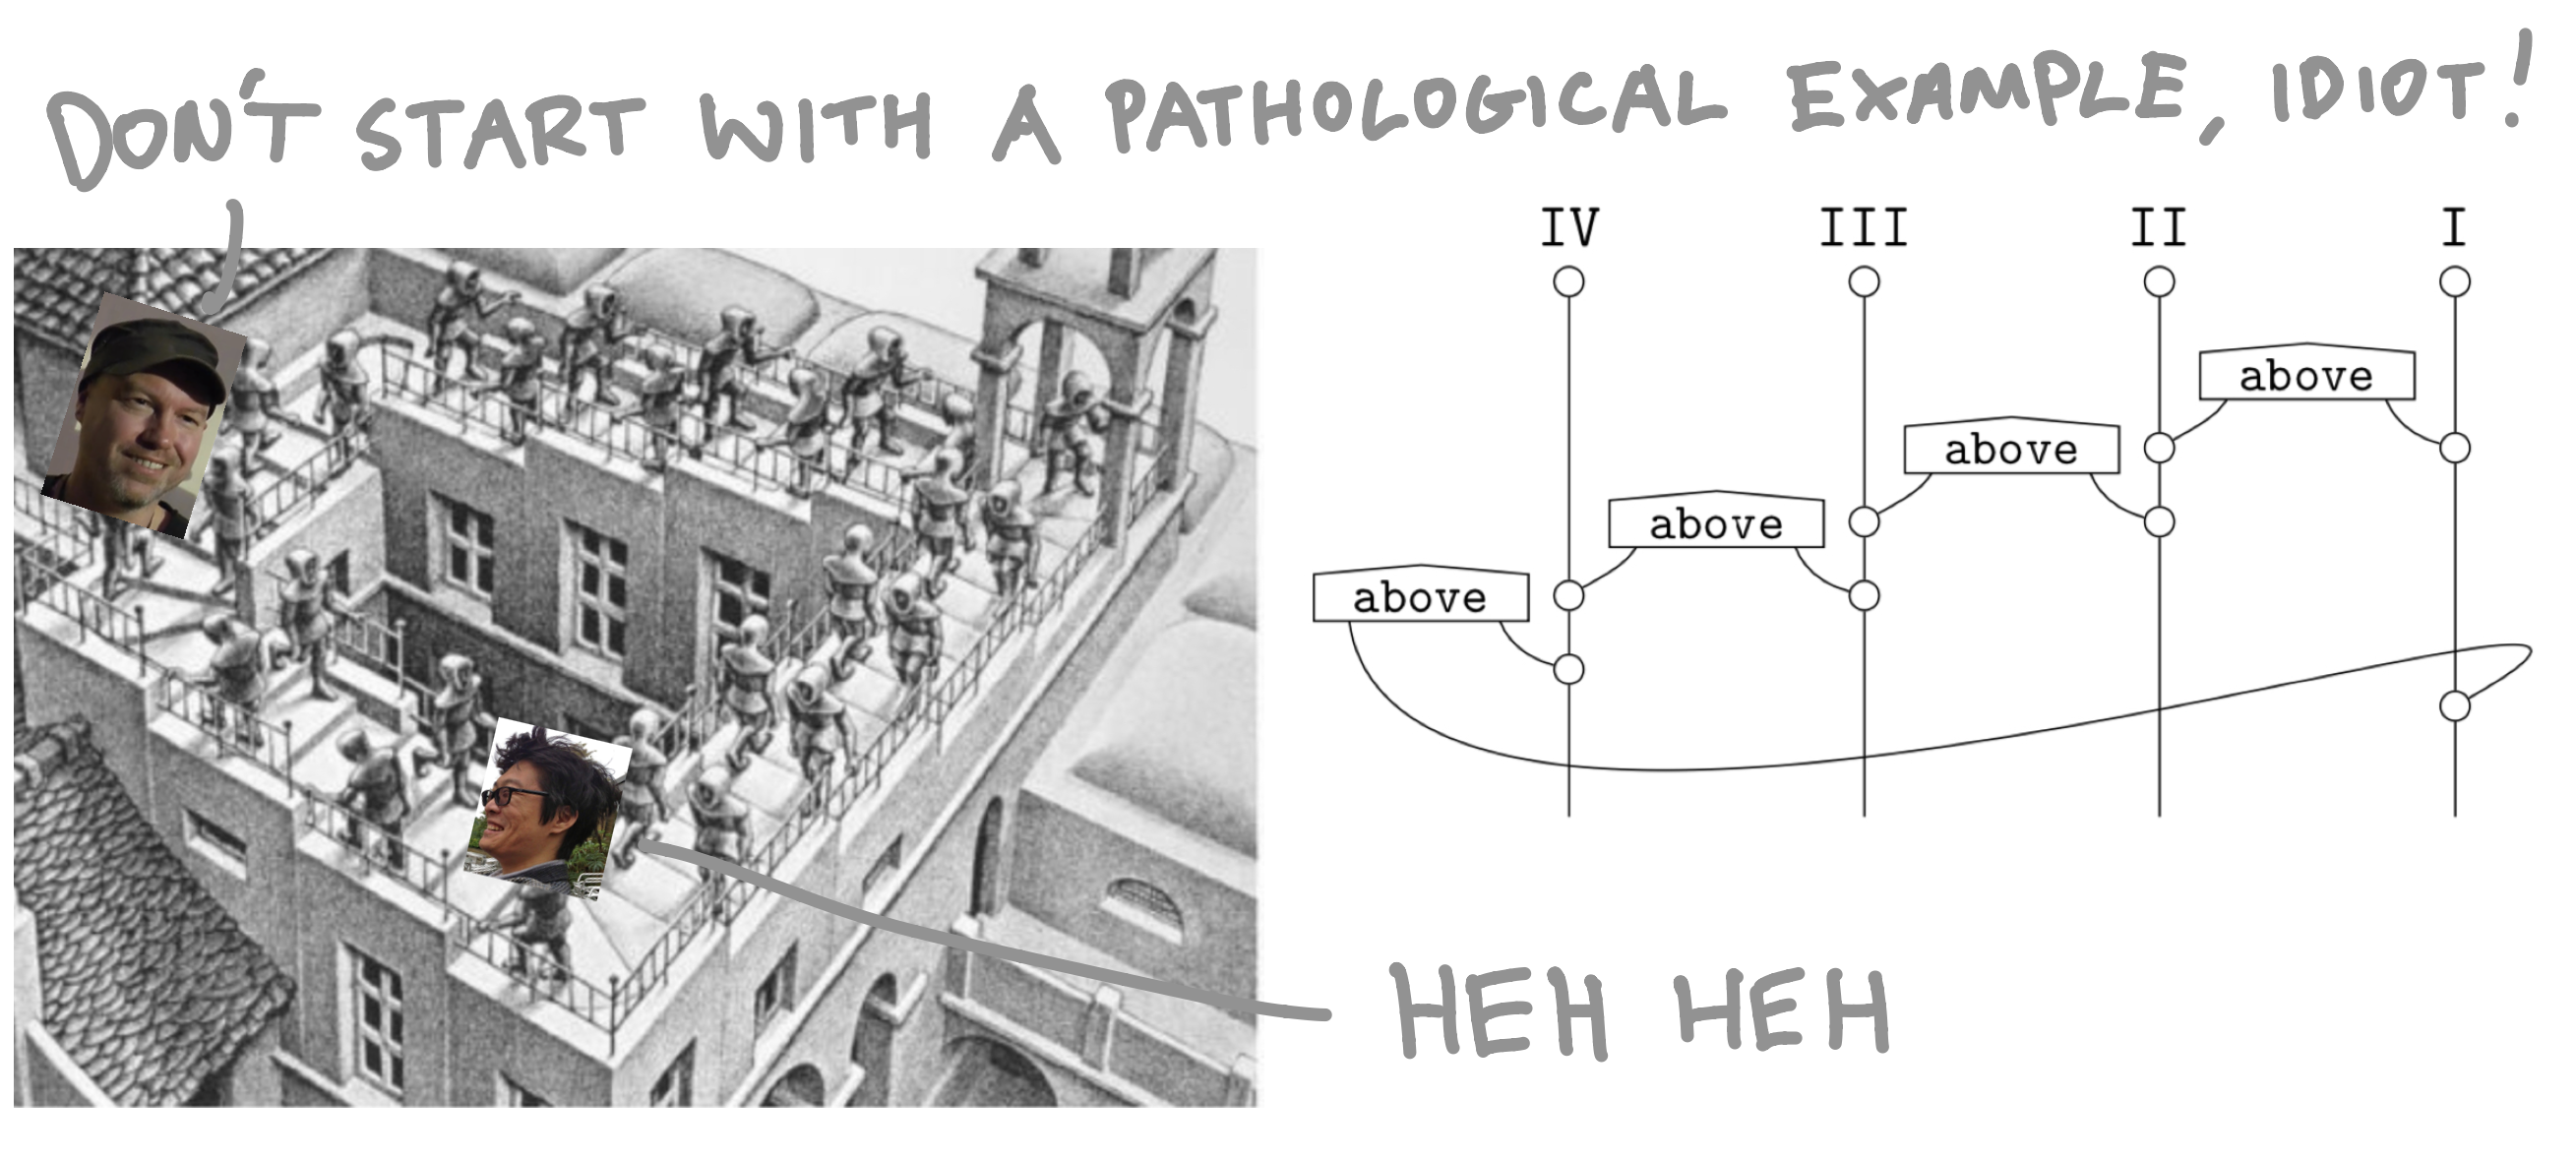
\includegraphics{figures/cartoons/space1}}
\caption{We wrote up the story about spaces in \bR CITE \e, the spiritual successor to \emph{interacting conceptual spaces I}. We could formally calculate the meanings of sentences that used linguistic spatial relations, all using a simple and tactile diagrammatic calculus.}
\end{figure}

\begin{figure}[h!]
\centering
\scalebox{1}{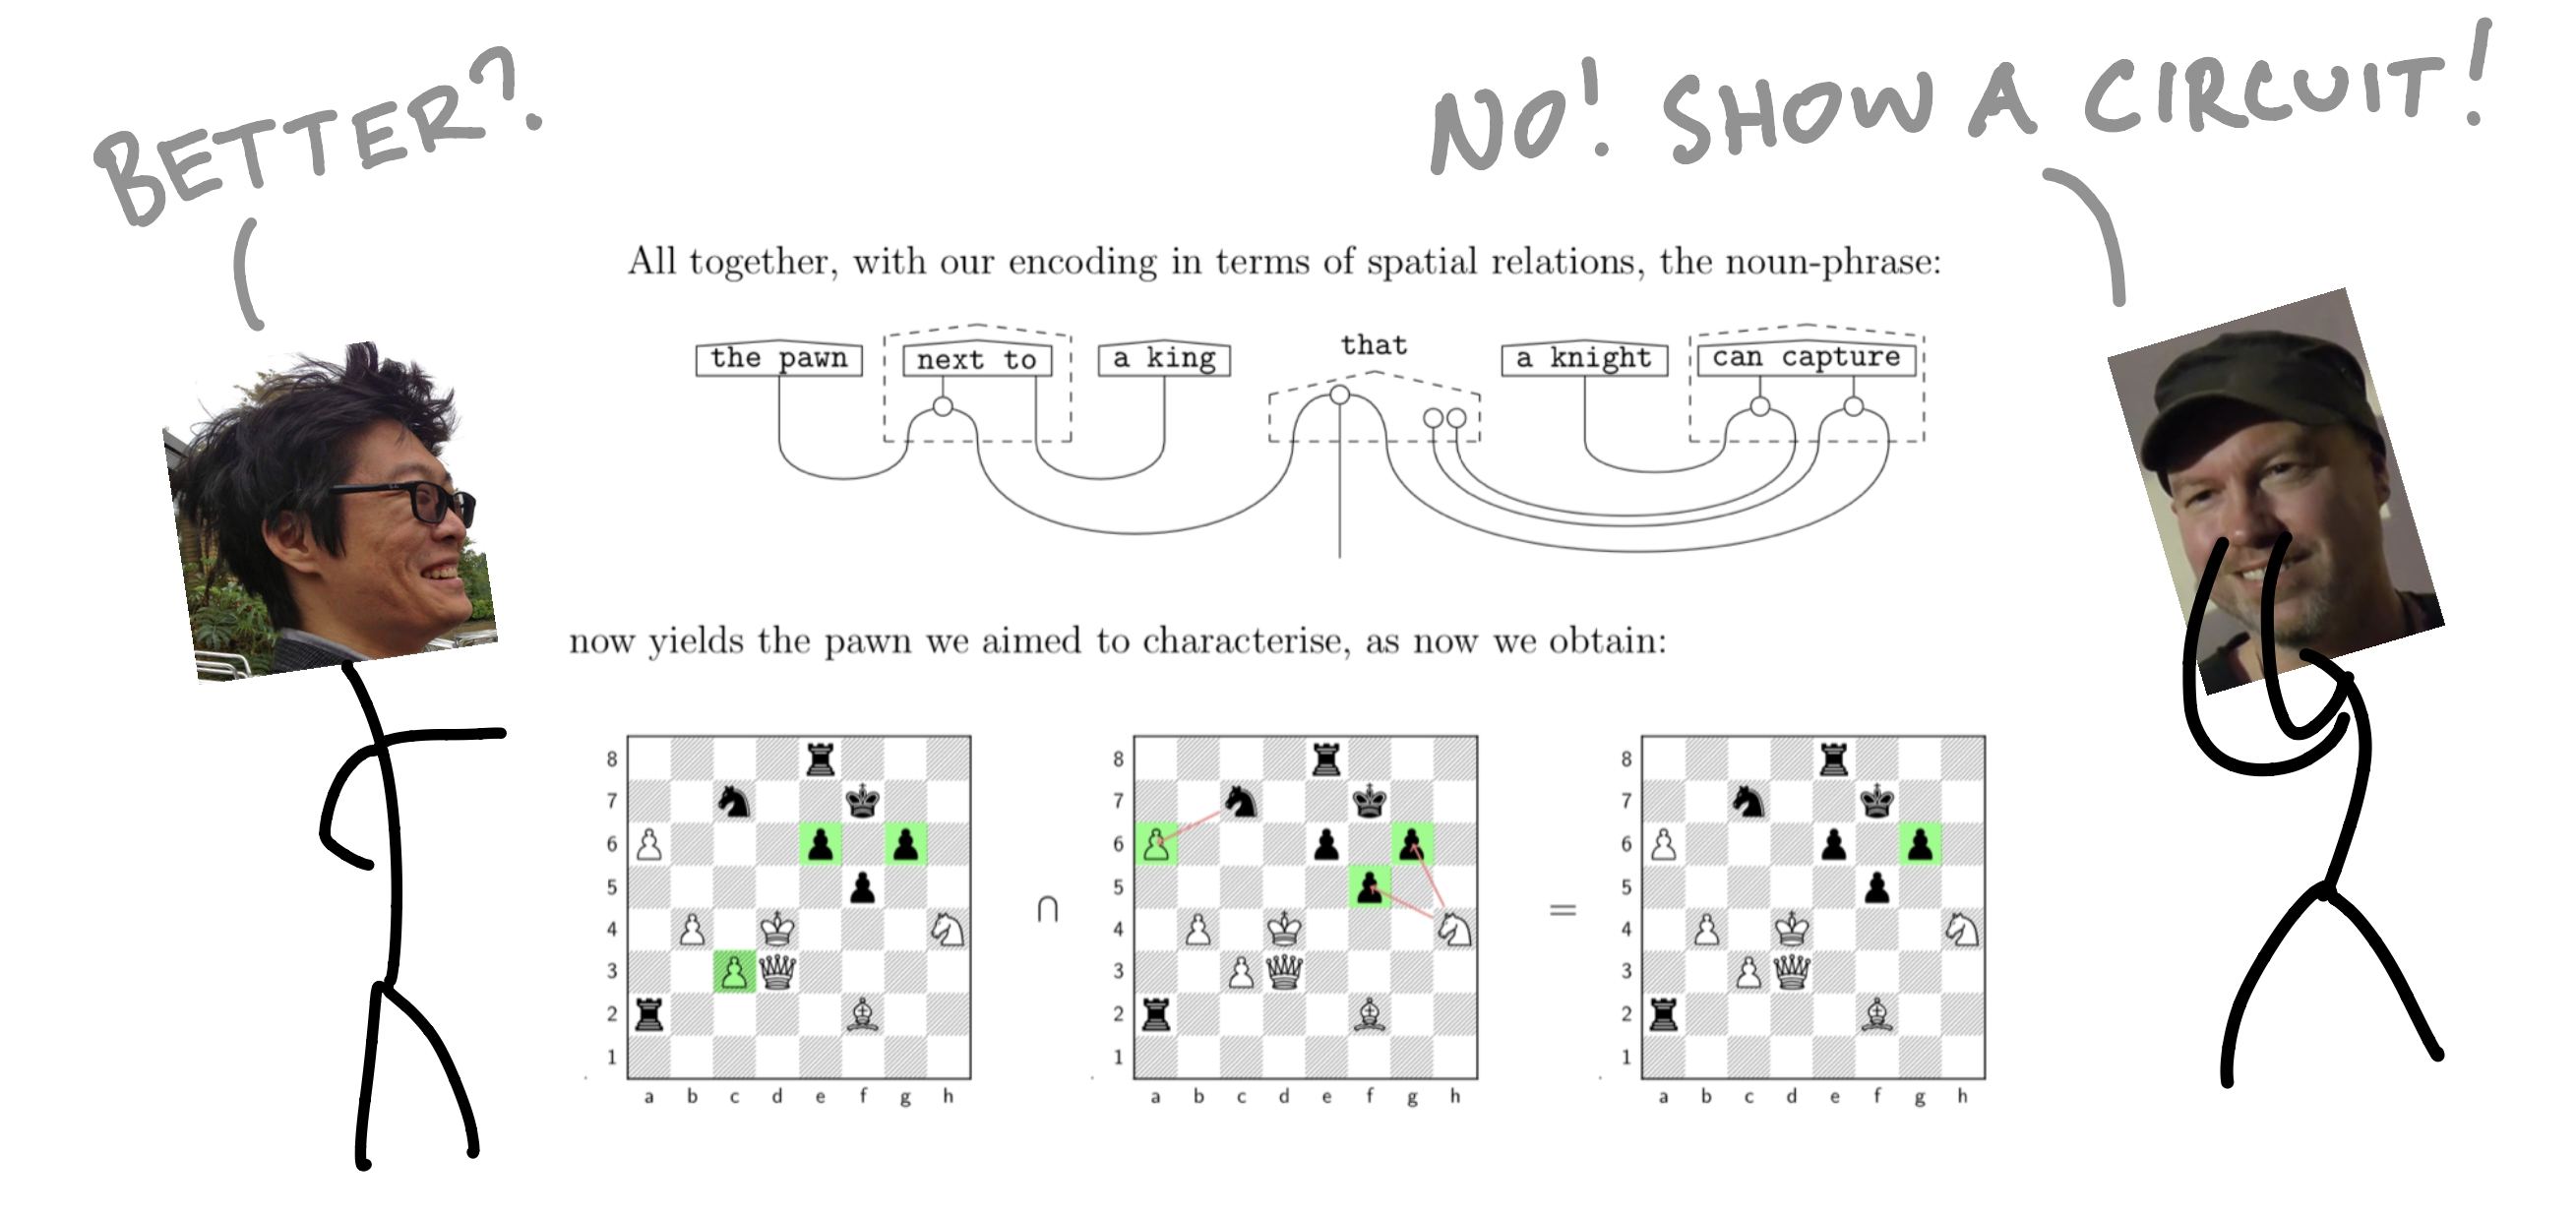
\includegraphics{figures/cartoons/space2}}
\end{figure}

\begin{figure}[h!]
\centering
\scalebox{1}{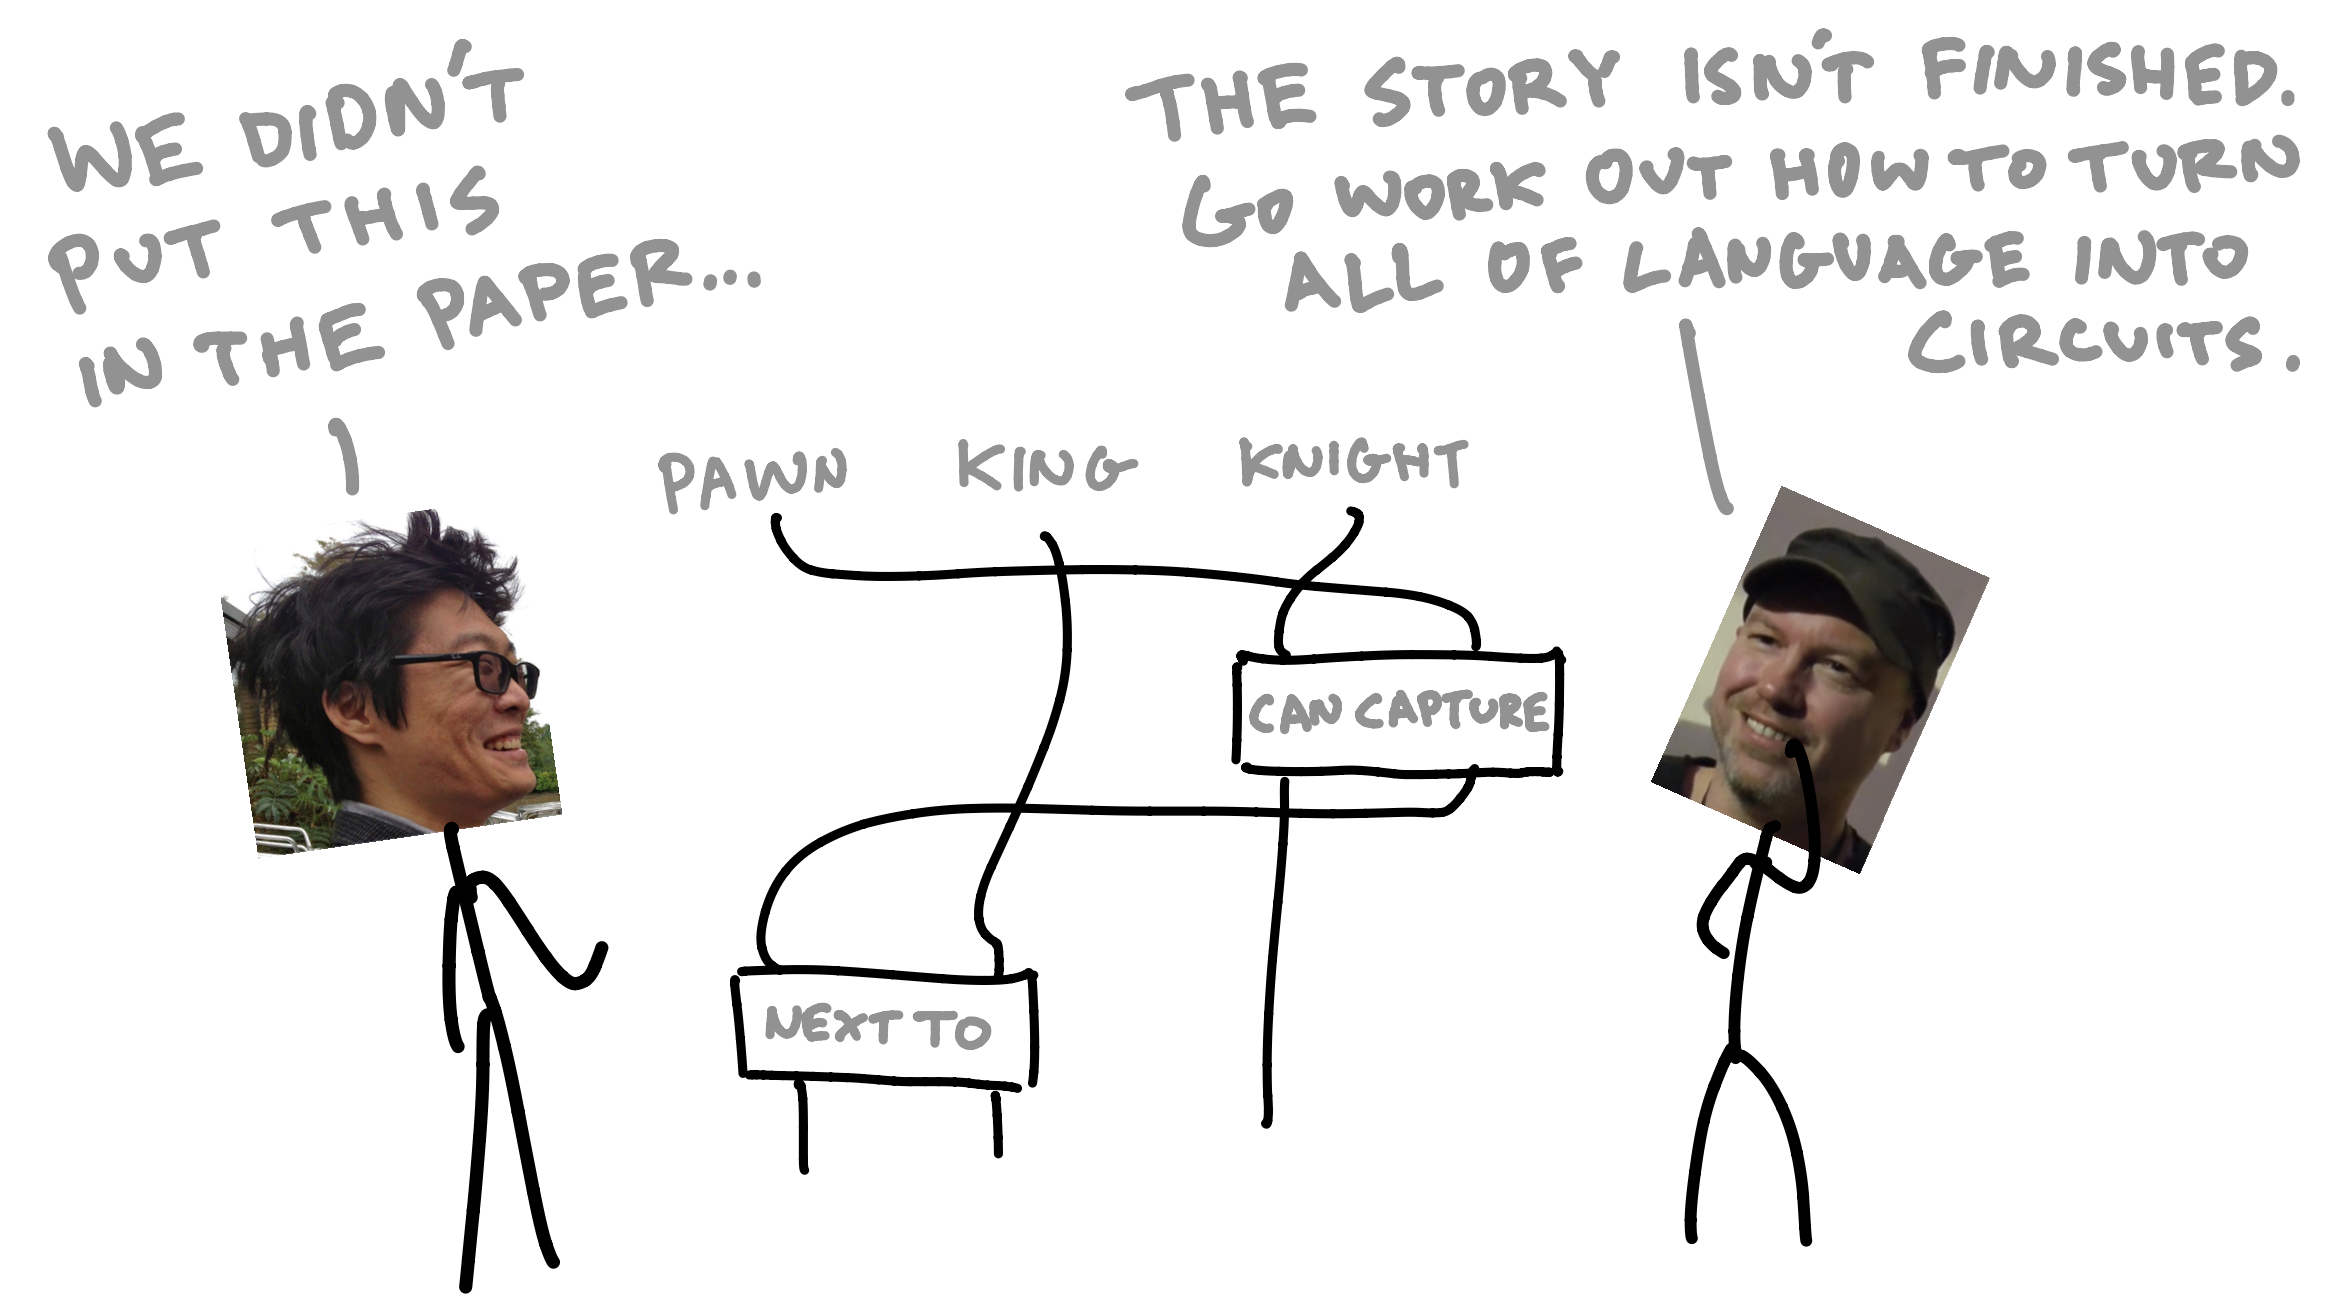
\includegraphics{figures/cartoons/space3}}
\caption{The paper on spatial relations actually came very late, because I was busy with Bob's ludicrous request to go turn "all of language" into circuits. I bitched and moaned about how I wasn't a linguist and how it was an impossible task, but I was in too deep to back out.}
\end{figure}

\begin{figure}[h!]
\centering
\scalebox{1}{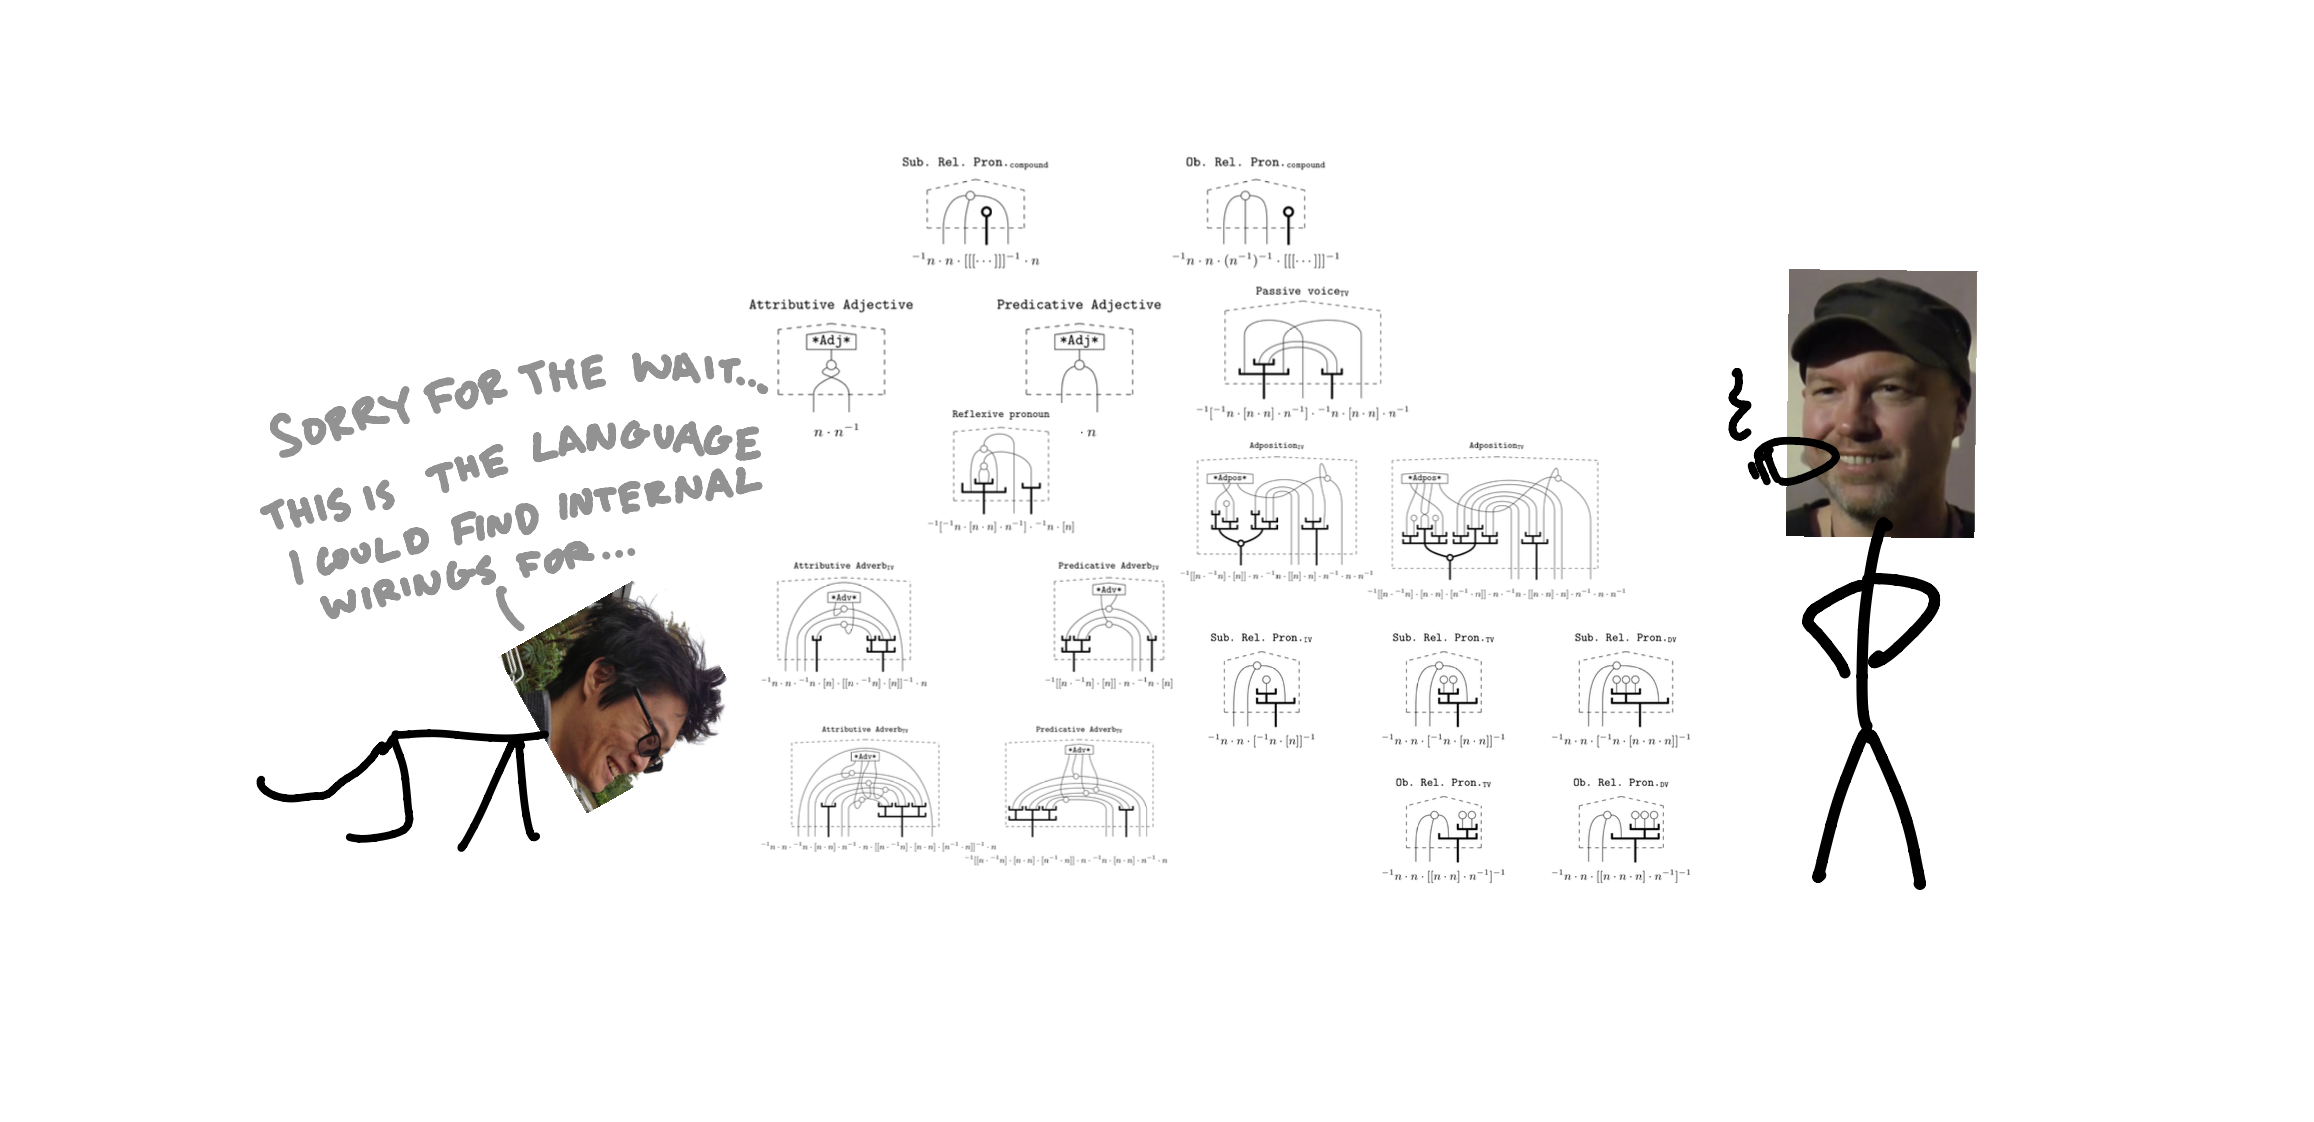
\includegraphics{figures/cartoons/pregroup1}}
\caption{I suppose the nice thing about aiming for the moon is that even failure might mean you leave orbit. So I settled for what I thought was a sensible fragment of English, for which I devised internal wirings and an algorithm that transformed pregroup diagrams with the internal wirings into circuit form. Many tiring diagrams later, I presented my results in the first draft of "distilling text into circuits".}
\end{figure}

\begin{figure}[h!]
\centering
\scalebox{1}{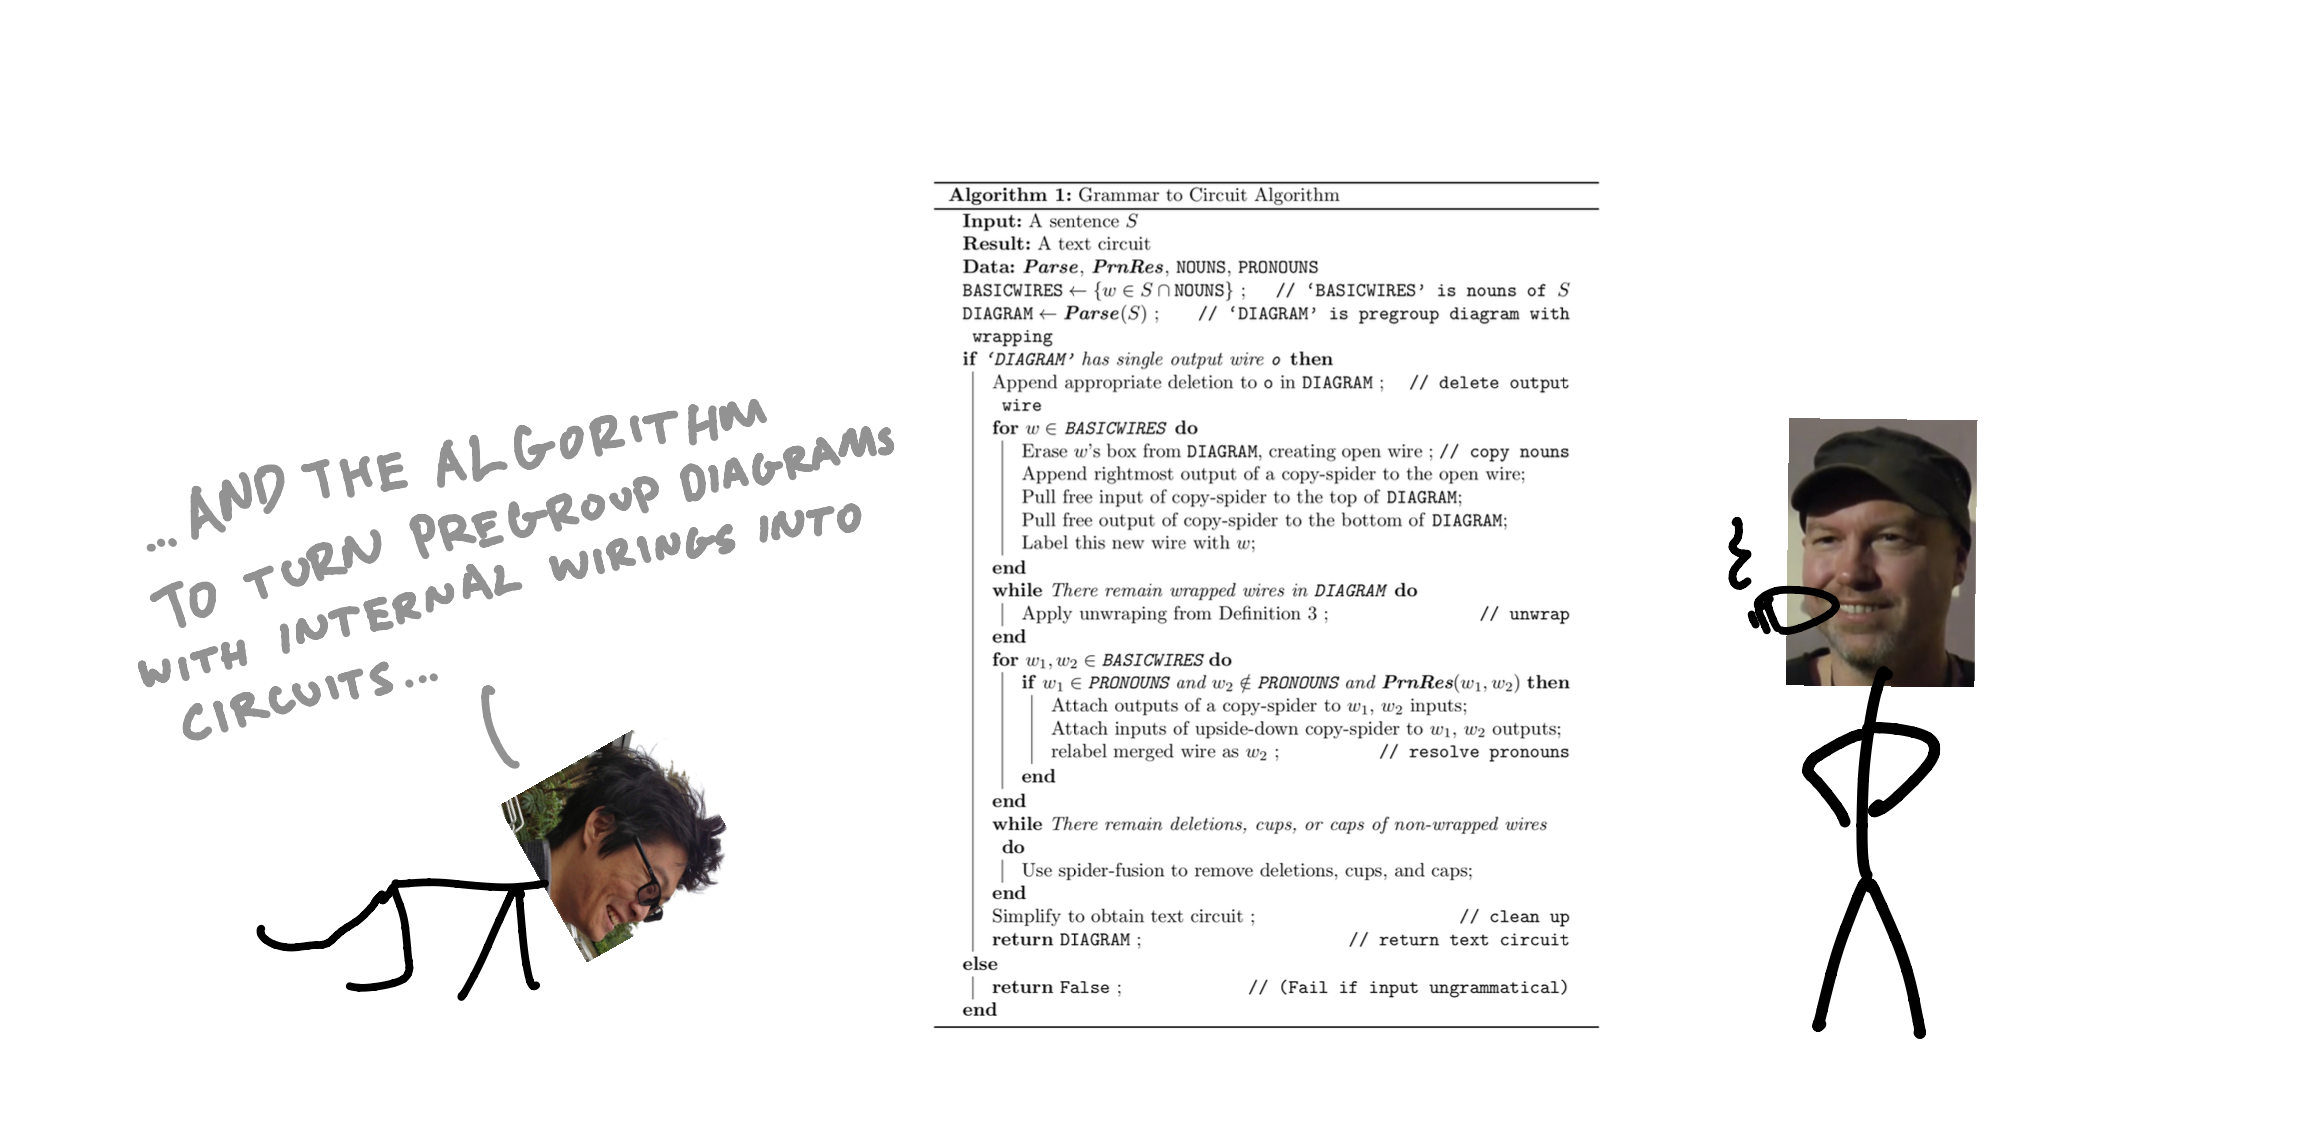
\includegraphics{figures/cartoons/pregroup2}}
\end{figure}

\begin{figure}[h!]
\centering
\scalebox{1}{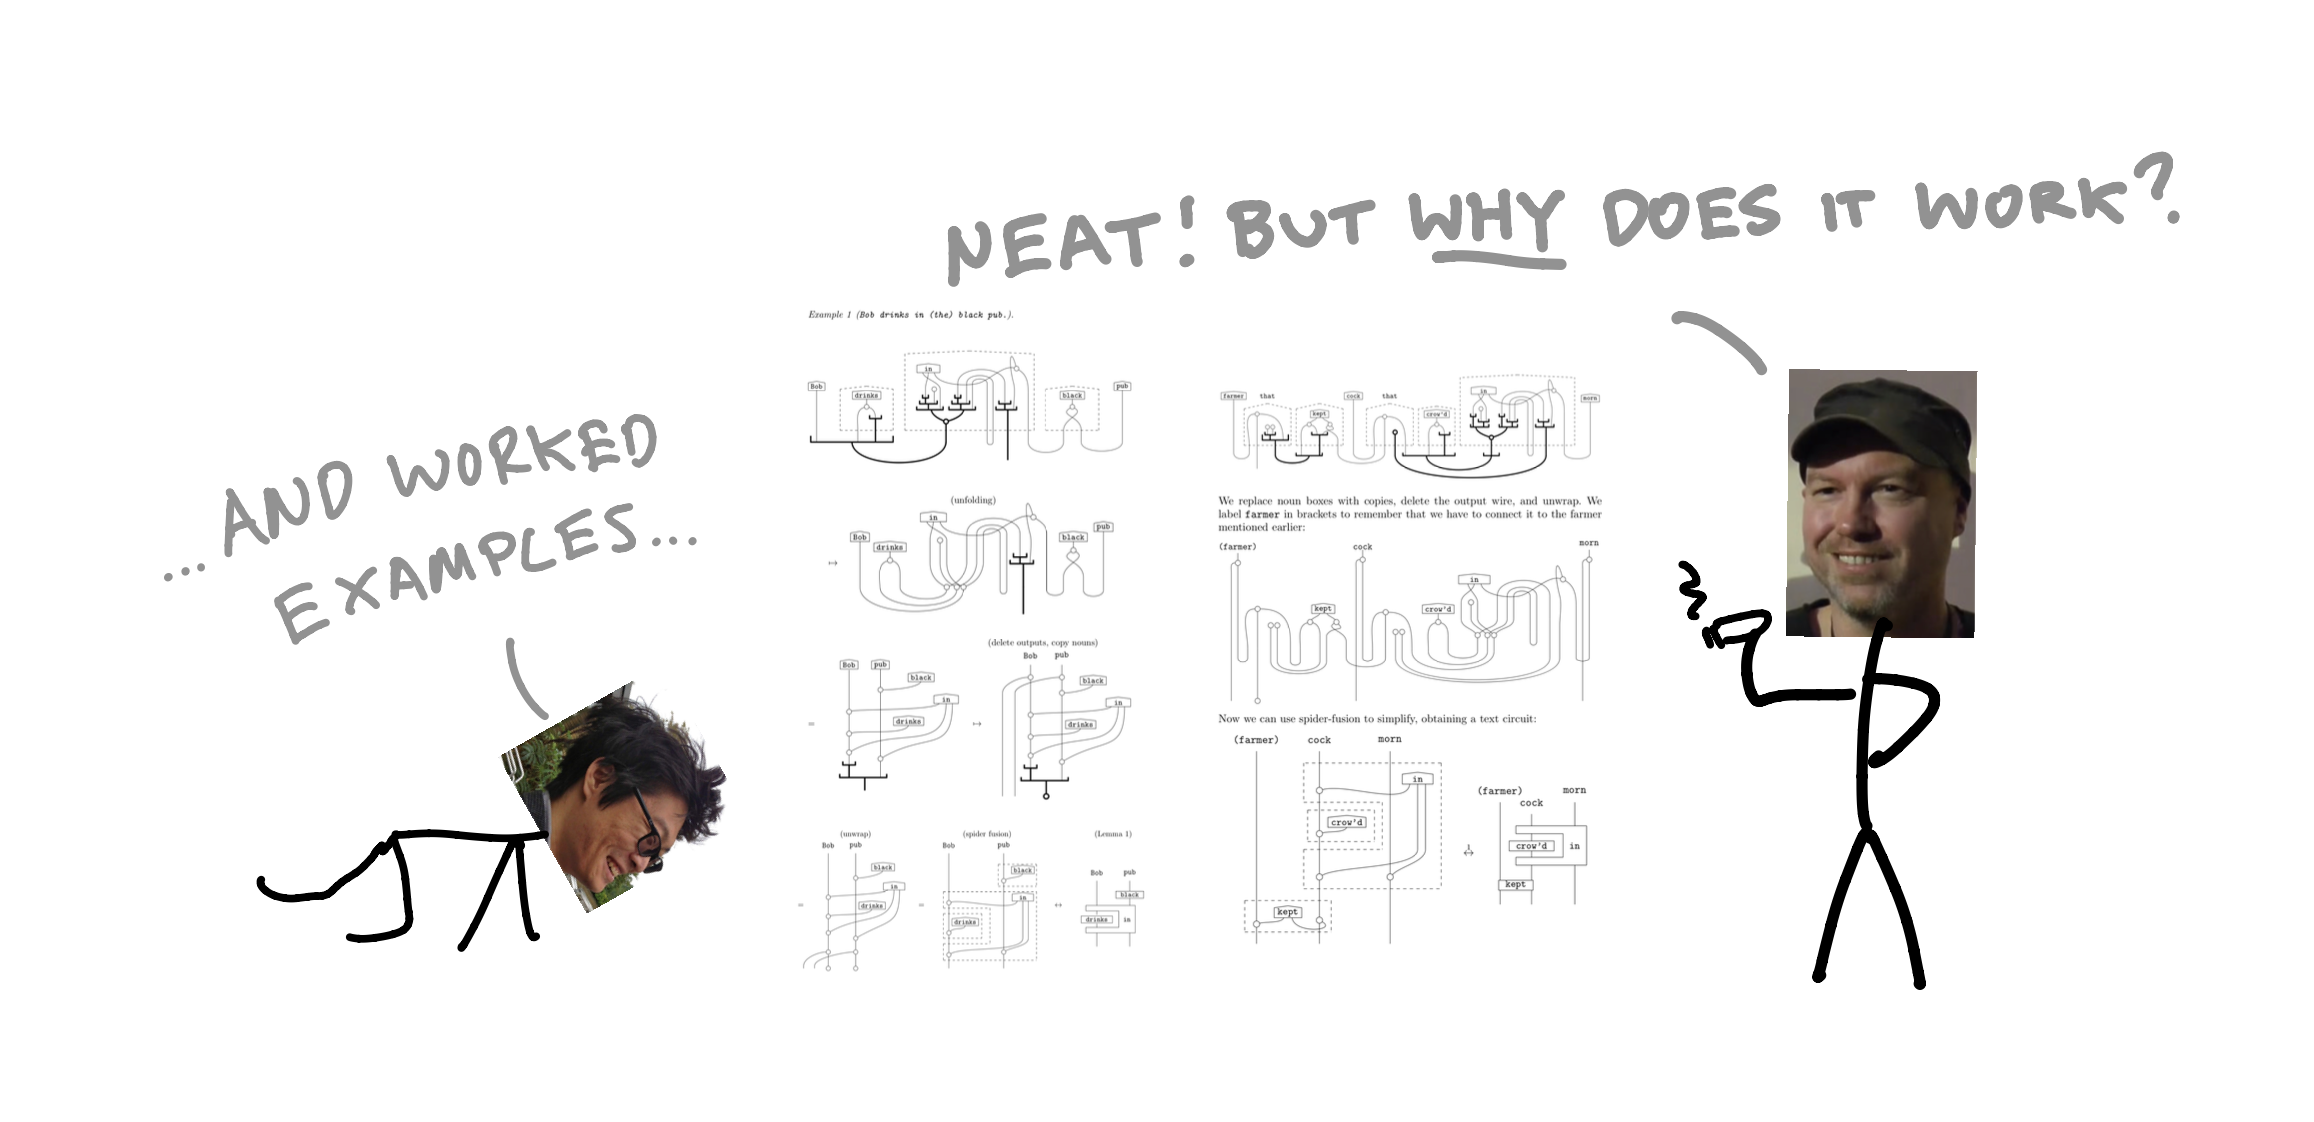
\includegraphics{figures/cartoons/pregroup3}}
\end{figure}

\begin{figure}[h!]
\centering
\scalebox{1}{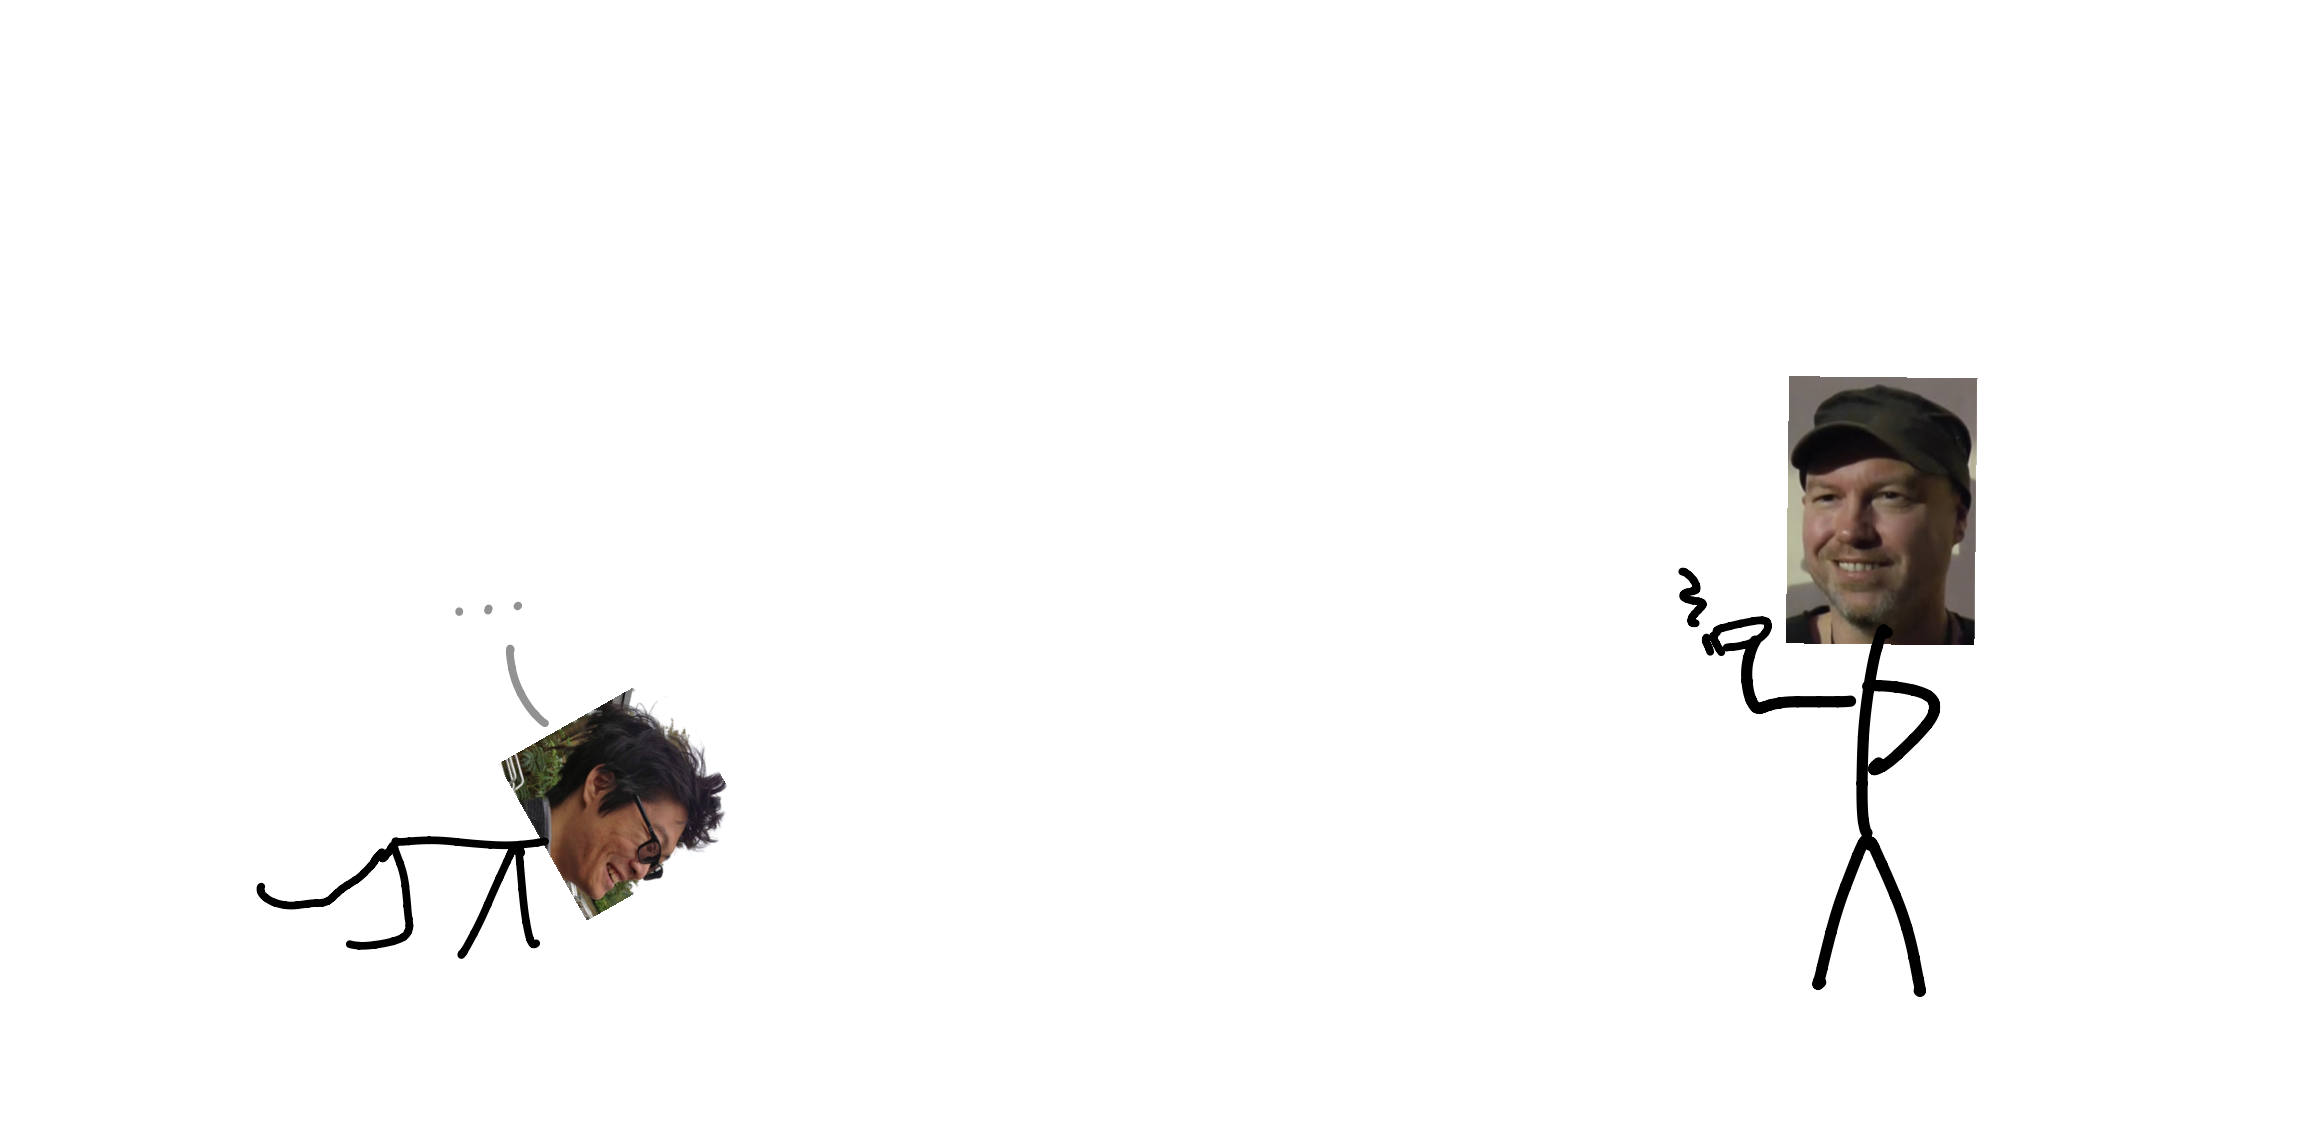
\includegraphics{figures/cartoons/pregroup4}}
\caption{Bob had a good point. Everything worked, but we had no understanding as to why, and accordingly, whether or not it would all break. At this point in time, Jonathon Liu, a masters' student I tutored during COVID, had committed the grave error of thinking diagrams were cool, and was now hanging out with me and Bob. After understanding the procedure, Jono independently devised the same arcane internal wirings as I had, but neither of us could explain how we did it. So we had evidence of an underlying governing structure that was coherent but inarticulable.}
\end{figure}

\begin{figure}[h!]
\centering
\scalebox{1}{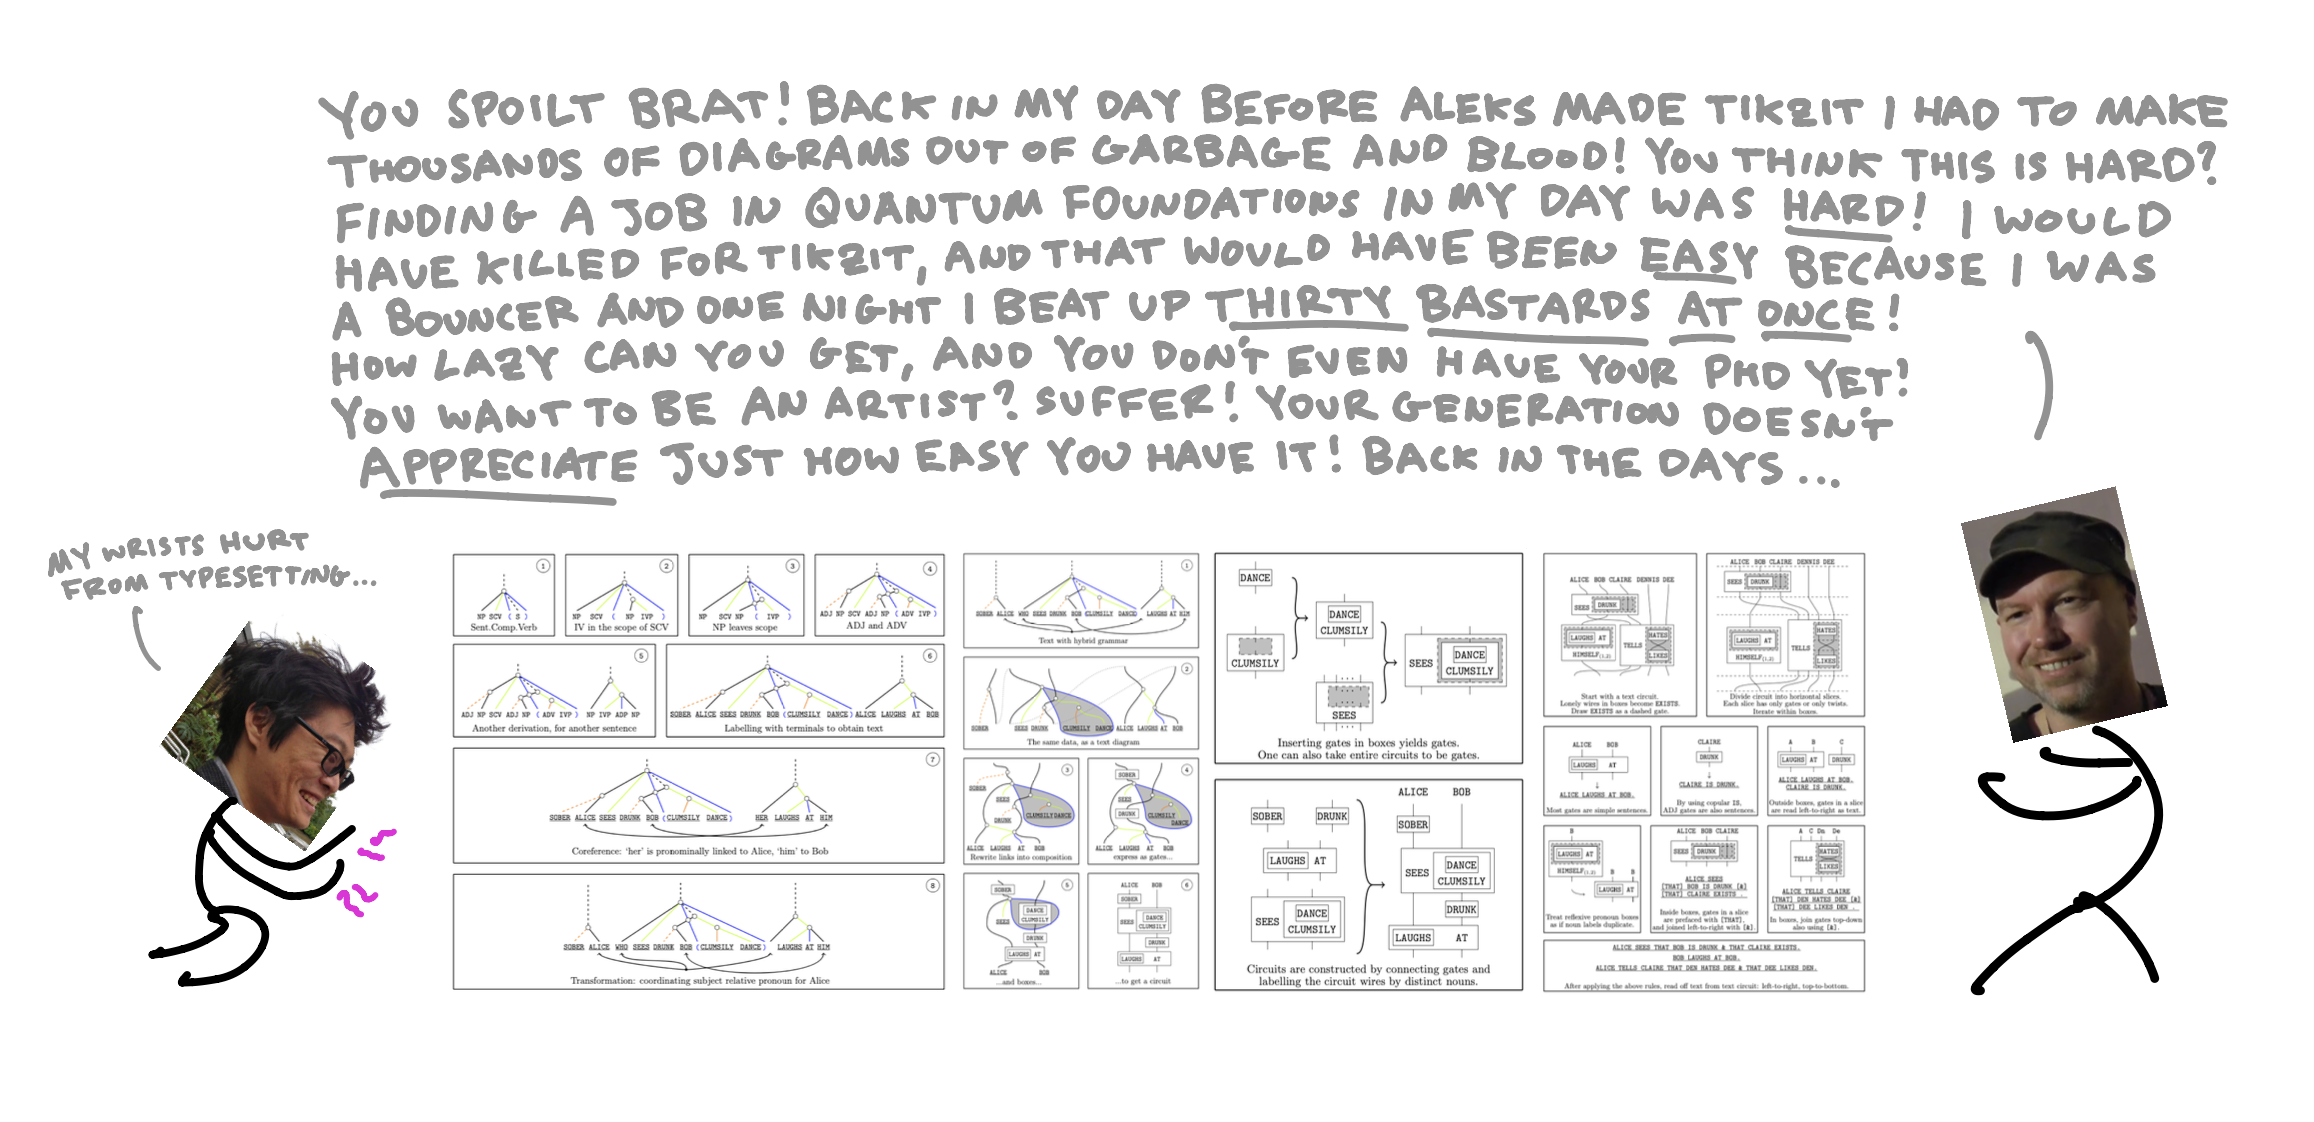
\includegraphics{figures/cartoons/bigpaper1}}
\caption{I realised that our intuitions were coming from an implicit productive grammar, rather than a parsing one, and that the path of least resistance for obtaining formal guarantees for the language-to-circuit procedure was to just handcraft a generative grammar for the fragment of language we were interested in. This meant scrapping everything in the first draft and starting again from scratch. Bob always had a word of gentle encouragement, giving me the motivation to persevere.\\

So now we had two ways to obtain text circuits. One from pregroups (which Jono had extended the technique for to CCGs in his master's thesis \bR CITE \e), and one from handcrafted productive grammars. Then came time for me to write my thesis, and there were three salient questions I wanted to address.\\
Firstly, what are internal wirings?\\
Secondly, how do text circuits relate to other generative grammars?\\
Thirdly, what are text circuits good for?\\
These questions are now what the rest of the thesis seeks to answer.
}
\end{figure}
%\clearpage
%\newpage
%\chapter{Corrections, as a letter to the reader}

Dear Reader,

How are you? I am well, thank you.

Forgive me for writing in this informal register; it is easier for me than the academic style (which I am no good at), and I would like to get these corrections done as painlessly as possible. You see, in the year or so it has taken for me to get around to these corrections, a lot has happened. I have gotten married, and I am soon to be a father. So I've learnt that there are more important things in life than a thesis, and I have otherwise been busy. While we are on apologies, please forgive me also for the tone of this work, which vacillates between serious and light; in my defense, I am constitutionally a trifler \cite{} (or else I wouldn't have gotten into formal linguistics), and I am still in the process of finding my voice as a writer.

There are several things I would like to get through in this letter, the main purpose of which is to settle most of the substantive corrections (recommended to me by my examiners Stefano Gogioso and Jules Hedges) in one go. I should preface by reminding you that all of this is written with a bit of distance from the rest of the work, and also that any opinions expressed here are strictly my own.

\section{Does it work?}

In the most important sense, no.

I will elaborate what I mean. There is a classical conception of structured approaches to AI/ML that permits capacities that go beyond what connectionist approaches are capable of, grounded in a kind of quasi-magical conception of mathematics as the ultimate form of understanding of --- and hence control over --- a phenomenon. It appears that part of the intellectual shock of generative AI is that one does not need to understand the mechanics of complicated phenomena in order to reliably induce them, given sufficient data and compute. This is obviously disappointing to many, and the highest sort of achievement that this thesis could have achieved is to have been a source of hope. Even a year ago the prospects seemed grim, and part of what took me so long to write the introduction was to compromise the positive vision from some demonstration of the complete superiority of structured approaches (basically no longer tenable after the advent of ChatGPT with RLHF) to something weaker, such as a performant way to synthesise structural/symbolic and connectionist approaches that has some other kind of benefit, such as "interpretability" (whatever that means.)

So taking \emph{"does it work?"} to mean \emph{"does it justify the activity of mathematically formulating the structure of language with respect to non-instrinsic measures of value (such as practical application)?"}, the answer is no, modulo most measures of value that people would care about. I say this because we've done some experiments.

\subsection{Have experiments been done?}

The approaches sketched out in Section \ref{} have been tried with neural networks in various ways by masters' students taking the Distributed Models of Meaning course offered in MFoCS here at Oxford, and separately it has been tried in the quantum setting \ref{} by talented scientists and engineers at the company at which I am employed at the time of writing. In the classical case, it works for some bAbI tasks, but at the cost of hardcoding the structure of the queries, and it doesn't outperform a transformer.

I could be wrong; it could be that all of the experiments done so far were in compute and data regimes that are too small to be indicative of how these approaches may scale. It could be that rather than the level of words and sentences there is some structural benefit to be obtained at the textual level, and so on, but I am not personally holding out hope any more. I do maintain that the symmetric monoidal (and hence string-diagrammatic) approach to formalising the structure of language is the best and most natural way to synthesise the mathematics with modern (practical) machine learning, so the fact that it doesn't work all that well leaves me with a very dim view of everything else. As a result of these experiments and other experiences, my own view of the role of structure has been further demoted. As far as natural language is concerned, at worst such structure appears to be some crutch for us humans: inductive biases that constrain and unnecessarily burden more sophisticated algorithms that can deal with the complexity of "the real world". At best, it appears to be tradeoff: computationally cheaper but worse answers.

\section{Can you situate this work with respect to the literature in formal linguistics?}

Look, it's not in the culture of my people to read \cite{}. It's either uninteresting so we put the book down, or if it is interesting, we put the book down and try to rederive it for ourselves. Accordingly, if armchair introspection was good enough for Harris and Chomsky and so on, I figured it was good enough for me too. Before I go on to do the scholarly thing, I'll reiterate what I told my examiners out of protest: I don't respect \emph{formal} linguists or their methods, in fact they disgust me, and I can hardly stand to look at even my own meagre work in the area. Since I'm probably the first (and, god willing for everyone's sake, the only) formal linguist to have used infinity-categories to model natural language syntax and to have provided a categorical semantics of metaphor starting from syntax, I defer to my own authority in concluding that the mathematics of formal linguistics in the literature (including this work) is not impressive, unfit for purpose, and not worth wasting any further time on. To be fair, I think there is a lot of interesting \emph{linguistics} out there --- in my mind the kind of distinction between formal versus respectable linguistics is exemplified by Daniel Everett uncovering the structure of Pirah\~{a} in the field, causing the formalist Chomsky to move the goalposts on what recursion means \cite{} --- but I have grown increasingly convinced that all of the effort to cast linguistics in mathematical terms up to now is best viewed as a kind of devotional or religious activity, a kind of benign way to kill time. Much like quantum computers at the moment, the only practical problem formal linguistics solves is the gainful employment of overeducated fools such as myself.

One way to summarise things is that the technical contents of this thesis point towards a nearby counterfactual history where all the linguists in the "Garden of Eden period" [Partee?] knew some of the modern structuralist mathematics that their programme obviously would have profited from. The fractiousness of linguists notwithstanding, it is my opinion that the interdisciplinarity of this thesis is accidental: from the perspective of the counterfactual history, the division of formal approaches to syntax and semantics (and some of the subdivisions thereof) would appear contrived. I am aware that this could come across as pretty arrogant and patronising talk, which is not my intention this time, because the point I am ultimately trying to make is that nothing in this thesis is particularly special, and could have been reinvented by anyone. Because I thought things through for myself for the most part, and since the relevant developments were due to collaborations with the similarly ignorant, text circuits and the other contents of this thesis owe no substantial intellectual debt to linguistics outside of perhaps Lambek and Firth, themselves far from the mainstream. Consequently, all of the parallels I am about to point out between the current stream of development and the main body of literature are independent rediscoveries. I take these parallels as indications of the "naturalness" of ideas that could have come about anytime and independently of specific individuals, and accordingly as evidence for the "nearbyness" of the counterfactual history I am trying to gesture at.

\subsection{Pregroups to Text Circuits vs. Transformational Grammar to Formal Semantics, as an addendum for the cartoon literature review}

The cartoon version of the literature review is folkloric, autochtonal, and maybe a little jingoistic: it is a caricature or myth of the field that we in it tell ourselves. I think that is sufficient for most readers, but if you are here, I owe you a critical and comparative retelling. In my view, the development of DisCoCat is only two minor counterfactuals removed from the lineage of mainstream formal semantics from Montague onto Heim \& Kratzer and onwards. Moreover, both of these counterfactuals rest only on the difference of when they began relative to the ambient development of mathematical formalisms and available computing.\\

\subsubsection{Counterfactual 1: Truth-conditional vs. Vectorial Semantics}

Montague semantics may be essentially characterised as the meeting of two ideas [CITE]: structure-preserving maps from syntax, and taking truth-conditions to be the essential data of semantics. On some accounts, only the former aspect of compositionality of semantics according to syntax is essential [CITE]. Accordingly, the first counterfactual is just the swapping of truth-conditional for vectorial semantics. Today there are several good reasons to prefer the latter over the former. First, the view that truth-conditions alone are the \emph{sine qua non} of natural language meanings has been incompatible with correspondence theories of truth at least since Barr fixed Putnam's permutation argument [CITE, CITE]. Second, vectors as lists-of-numbers are more expressive and computationally practical, so much so in its current form that the very need for a formal account of "semantics" is put to question. Third, with a rare few exceptions, the truth-conditional programme and its descendents are bankrupt, and worse, have terrible mathematical taste. A lot of mathematical structure has been marshalled [CITE,CITE,CITE] to salvage the programme by trying to force intensions and pragmatics and everything-in-the-world into the propositional mould, and it is unclear what all of this mathematics buys us except for more of the same. In practical terms, the increasing extent to which statistical language models adequately handle semantics exactly matches the decreasing extent to which a complicated mathematical account of the same is warranted, and in theoretical terms it would be definitionally preposterous to seriously assert that the study of the mathematical models themselves lends insight into the phenomena they are intended to be surrogates for.

But all this criticism can only be said with the benefit of hindsight, and to give credit, it all must have seemed like a very good idea at the time. A model-theoretic, truth-conditional account of semantic data was the natural choice for a concrete target for the structure-preserving map, I speculate, for several reasons: Montague himself was a logician, and truth-conditions were at once flexible enough to capture (to a logician's satisfaction) some semantic phenomena of interest, while being amenable to computation \emph{by hand}, as was necessarily the case at the time owing to the lack of computers. Certainly there was adequate sophistication manipulating vectors by that time as well, but the vectorial view would have been more difficult to calculate with, even restricted to a setting without nonlinearities. It could be argued that, in any case, vectorial semantics in the form of word-embeddings requires a degree of data-storage and computing faculties that would not have been available until fairly recently. Moreover, even the theoretical soil was arguably unready: category theory was insufficiently spread and understood, and hence a broadly accessible mathematical understanding of structure and structure-preservation outside of particular concrete instances was unavailable.

\subsubsection{Counterfactual 2: Generative vs. Typelogical views of syntax}

- the usual mathematical conception of syntax is combinatoric --- see formal language theory.
-- now "generative" in some circles is just synonymous with "formal", but there is the original sense in which mathematical machinery generates correct sentences.
- the typelogical alternative is the proof-theoretic counterpart to a combinatoric conception, where parsing rather than generation takes precedence.
- parsing is the more practical thing for computers; compare to generation, where it becomes very complicated to make generation dependent on a semantic basis.

\subsection{Confession: Criticisms of Quantum Linguistics (and of the Academic-Industrial complex more generally)}

In light of the above counterfactuals, here are two implications of the quantum linguistics myth that I wish to dismiss here. The first that is often touted is that there is some kind of fruitful and practical synthesis to be won from the meeting of grammatical structure and vectorial semantics. This is the same kind of professionally-sensible claim that certain mathematicians will sometimes make in other domains too: that a deep consideration of structure will ultimately pay practical dividends. As far as I can tell in the case of DisCo and offshoots, this hasn't yet been demonstrated to be true. There's just no setting we know of, classicial or quantum, where deliberately introducing grammatical structure helps with any practical task, and shifting the goalposts to interpretability or whatever else has not worked either. So it isn't for lack of technical ability or imagination, it just appears to be that anything you could have done with "structure" or "composition" you could have also done without. This isn't to say that the structural view is totally without merit --- it is certainly more human-friendly and aids in Interpretability writ large as subsuming pedagogy and communication --- it's just impractical. This was surprising and disappointing for me, because of a more deep-seated belief in myself I have had to kill, that \emph{structure is magic}. If you are a computational linguist, I welcome you to try synthesising your structural formalisms with vectorial semantics across similar bridges as are built here, and I would be happy to be proved wrong about the importance and power of structure: the disenchanted view that I currently hold is that adding structure is in general a way to get computationally cheaper but worse answers.

There is a second, unspoken implication that is more seductive; that there exists some deep and fundamental unity between quantum theory and natural language. This is a rather commonplace sin more generally, that in some field XYZ with relatively little mathematical sophistication someone will steal the valour of physics by squatting on "Quantum XYZ", or "Quantum-inspired XYZ", when all they really mean is e.g. the use of noncommuting operators or tensor products or density matrices or some other narrow mathematical facet of quantum theory. Such views by themselves may be harmless, but in conjunction with the vaguely held but common assumption of mathematical realism [CITE], we find ourselves in trouble. The extent to which there are quantum theories of linguistics or cognitive science or anything else deep and multifaceted is that there are mathematical paintbrushes that have been used to illustrate quantum theory with which we can also better sketch and appreciate certain limited phenomena in other domains. However, even this honest appraisal is co-opted by a blameless form of motte-and-bailey, where a serious faction will disavow mysticism, but the field as a whole survives by luring na\"{i}ve researchers with the seductive implication.

These objections would usually be fatal, but as it goes, the alternatives are no better; mostly worse. In fact, any defensive manoeuvre that works to justify formal linguistics as an academic activity or otherwise will provide cover for quantum linguistics too, with minor modifications such as swapping out "quantum" for some exotic dialect of logic. I think that's worth reiteration: if you think what I'm saying about quantum linguistics is bad, consider that the rest of formal linguistics is worse off in terms of what it actually does, or the kind of understanding that is gained. As a personal aside, and not referring to any subfield in particular, I think this sort of dysfunction is a natural consequence of the sociology of academic and industrial research. Insofar as academia generally (1-) does not have the resources to turn theory into practice and that (2-) there is pressure to publish, there is an understandable incentive for theorists to (-2) tell stories valued according to doctrinal measures of niceness, with (-1) no corresponding selection pressure for whether those stories actually translate to anything in the real world. It is actually a na\"{i}ve view --- based on the simpleminded belief that valuation corresponds to effective technology --- that these myths crafted in ivory towers immediately perish in the sunlight of a free market economy. While these myths are endless sources of pain for the engineers who must bring them into fruition, they are crucial memetic pillars for kayfabe or some other epistemic asymmetry that keeps morale high for the technically uninitiated, which includes investors. In this sense academics and capital are natural allies against embattled engineers and builders, an observation which might serve as a sufficient axiom to deduce and explain much of the dynamics of the academic-industrial complex.

\subsection{On Deep Structure, the Universal Base Hypothesis, and the "Lexical Objection"}

???

\subsection{On communication, and the mathematical infeasibility of the Autonomy of Syntax}

\subsection{On frameworks for rewriting systems}

\subsection{On formality in cognitive semantics}


\bibliographystyle{alpha}
\bibliography{thesis_intro}





\end{document}